% CREATED BY DAVID FRISK, 2016
% MODIFIED BY JAKOB JARMAR, 2016
% A few changes by Birgit Grohe, 2017 and 2018
% Adjustments with the help of Gustav Örtenberg 2019
% Parskip % bibliography system updated by Erik Ljungdahl, May 2022

% IMPORT SETTINGS
\documentclass[12pt,a4paper,twoside,openright]{report}
% CREATED BY DAVID FRISK, 2016

% BASIC SETTINGS
\usepackage{moreverb}								% List settings
\usepackage{textcomp}								% Fonts, symbols etc.
\usepackage{lmodern}								% Latin modern font
\usepackage{helvet}									% Enables font switching
\usepackage[T1]{fontenc}							% Output settings
\usepackage[english]{babel}							% Language settings
\usepackage[utf8]{inputenc} 						% Input settings
\usepackage{textcomp}
\usepackage{lmodern}

\usepackage{ bbold }

\usepackage{amsmath}								% Mathematical expressions (American mathematical society)
\usepackage{amssymb}								% Mathematical symbols (American mathematical society)
\usepackage{mathtools}								% Mathematical symbols (American mathematical society)
% for drawing wiring diagrams
\usepackage{tikz}
\usetikzlibrary{ 
    cd,
    math,
    decorations.markings,
    decorations.pathreplacing,
    positioning,
    arrows.meta,
    shapes,
    shadows,
    shadings,
    calc,
    fit,
    quotes,
    intersections,
    circuits,
    circuits.ee.IEC,
    external
    }
% \tikzexternalize[prefix=tikz/]

\pgfdeclarelayer{edgelayer}
\pgfdeclarelayer{nodelayer}
\pgfsetlayers{edgelayer,nodelayer,main}



\tikzset{
	tick/.style={postaction={
  	decorate,
    decoration={markings, mark=at position 0.5 with
    	{\draw[-] (0,.4ex) -- (0,-.4ex);}}}
  }
} 

\tikzset{
biml/.tip={Glyph[glyph math command=triangleleft, glyph length=.87ex]},
bimr/.tip={Glyph[glyph math command=triangleright, glyph length=.92ex]},
}

\newcommand{\bimodto}[1][]{
	\begin{tikzcd}[ampersand replacement=\&, cramped]\ar[r, biml-bimr, "#1"]\&~\end{tikzcd}  
}
\newcommand{\bimodfrom}[1][]{
	\begin{tikzcd}[ampersand replacement=\&, cramped]\ar[r, bimr-biml, "#1"]\&~\end{tikzcd}  
}

  
\tikzset{trees/.style={
	inner sep=0, 
	minimum width=0, 
	minimum height=0,
	level distance=.5cm, 
	sibling distance=.5cm,
%	every child/.style={fill},
	edge from parent/.style={shorten <= -2pt, draw, ->},
	grow'=up,
	decoration={markings, mark=at position 0.75 with \arrow{stealth}}
	}
}
\newcommand{\idchild}{edge from parent[double, -]}
  	
  \tikzset{
     oriented WD/.style={%everything after equals replaces "oriented WD" in key.
        every to/.style={out=0,in=180,draw},
        label/.style={
           font=\everymath\expandafter{\the\everymath\scriptstyle},
           inner sep=0pt,
           node distance=2pt and -2pt},
        semithick,
        node distance=1 and 1,
        decoration={markings, mark=at position \stringdecpos with \stringdec},
        ar/.style={postaction={decorate}},
        execute at begin picture={\tikzset{
           x=\bbx, y=\bby,
           }}
        },
     string decoration/.store in=\stringdec,
     string decoration={\arrow{stealth};},
     string decoration pos/.store in=\stringdecpos,
     string decoration pos=.7,
	 	 dot size/.store in=\dotsize,
	   dot size=3pt,
	 	 dot/.style={
			 circle, draw, thick, inner sep=0, fill=black, minimum width=\dotsize
	   },
     bbx/.store in=\bbx,
     bbx = 1.5cm,
     bby/.store in=\bby,
     bby = 1.5ex,
     bb port sep/.store in=\bbportsep,
     bb port sep=1.5,
     % bb wire sep/.store in=\bbwiresep,
     % bb wire sep=1.75ex,
     bb port length/.store in=\bbportlen,
     bb port length=4pt,
     bb penetrate/.store in=\bbpenetrate,
     bb penetrate=0,
     bb min width/.store in=\bbminwidth,
     bb min width=1cm,
     bb rounded corners/.store in=\bbcorners,
     bb rounded corners=2pt,
     bb small/.style={bb port sep=1, bb port length=2.5pt, bbx=.4cm, bb min width=.4cm, 
bby=.7ex},
		 bb medium/.style={bb port sep=1, bb port length=2.5pt, bbx=.4cm, bb min width=.4cm, 
bby=.9ex},
     bb/.code 2 args={%When you see this key, run the code below:
        \pgfmathsetlengthmacro{\bbheight}{\bbportsep * (max(#1,#2)+1) * \bby}
        \pgfkeysalso{draw,minimum height=\bbheight,minimum width=\bbminwidth,outer 
sep=0pt,
           rounded corners=\bbcorners,thick,
           prefix after command={\pgfextra{\let\fixname\tikzlastnode}},
           append after command={\pgfextra{\draw
              \ifnum #1=0{} \else foreach \i in {1,...,#1} {
                 ($(\fixname.north west)!{\i/(#1+1)}!(\fixname.south west)$) +(-
\bbportlen,0) 
  coordinate (\fixname_in\i) -- +(\bbpenetrate,0) coordinate (\fixname_in\i')}\fi 
  %Define the endpoints of tickmarks
              \ifnum #2=0{} \else foreach \i in {1,...,#2} {
                 ($(\fixname.north east)!{\i/(#2+1)}!(\fixname.south east)$) +(-
\bbpenetrate,0) 
  coordinate (\fixname_out\i') -- +(\bbportlen,0) coordinate (\fixname_out\i)}\fi;
           }}}
     },
     bb name/.style={append after command={\pgfextra{\node[anchor=north] at 
(\fixname.north) {#1};}}}
  }
  

\newcommand{\boxofbullets}[6][1]{% [y-spacing] {number of bullets} {left endpoint} {label} {text} {position}
	\foreach \i [evaluate=\i as \y using {#1/2*((#2-1)/2-\i)}] in {1,...,#2}{
		\node (pt_#4_\i) at ($(0,\y)+#3$) {$\bullet$};
		\node[#6, font=\tiny] (lab_#4_\i) at ($(0,\y)+#3$) {#5$_\i$};
	}
	\node[draw, rounded corners, inner xsep=2pt, inner ysep=0pt, fit={(pt_#4_1) (pt_#4_#2) (lab_#4_1) (lab_#4_#2)}] (box_#4) {};
}

\tikzset{polybox/.style={
	poly/.style ={
  	rectangle split, 
  	rectangle split parts=2, 
		rectangle split part align={bottom},
  	draw, 
  	anchor=south, 
  	inner ysep=4.5,
	  prefix after command={\pgfextra{\let\fixname=\tikzlastnode}},
		append after command={\pgfextra{
			\node[inner xsep=0, inner ysep=0, 
				fit=(\fixname.north west) (\fixname.two split east)] 
				(\fixname_dir) {};
			\node[inner xsep=0, inner ysep=0, 
				fit=(\fixname.south west) (\fixname.two split east)] 
				(\fixname_pos) {};
			}}
	},
	dom/.style={
		rectangle split part fill={none, blue!10}
	}, 
	cod/.style={
		rectangle split part fill={blue!10, none}
	},
	constant/.style={
		rectangle split part fill={red!50, none}
	},
	identity/.style={
		rectangle split part fill={gray, gray}
	},
	linear/.style={
		rectangle split part fill={gray, none}
	},
	linear dom/.style={
		rectangle split part fill={gray, blue!10}	
	},
	linear cod/.style={
		rectangle split part fill={blue!10!gray, none}	
	},
	pure/.style={
		rectangle split part fill={none, gray}
	},
	pure dom/.style={
		rectangle split part fill={none, blue!10!gray}
	},
	pure cod/.style={
		rectangle split part fill={blue!10, gray}
	},
	shorten <=3pt, shorten >=3pt,
	first/.style={out=0, in=180},
	climb/.style={out=180, in=180, looseness=2},
	climb'/.style={out=0, in=0, looseness=2},
	last/.style={out=180, in=0},
	mapstos/.style={arrows={|->}},
	tos/.style={arrows={->}},
	font=\footnotesize,
	node distance=2ex and 1.5cm
}
}

\tikzset{
biml/.tip={Glyph[glyph math command=triangleleft, glyph length=1.05ex]},
bimr/.tip={Glyph[glyph math command=triangleright, glyph length=1.1ex]},
}





\newcommand{\earpic}{
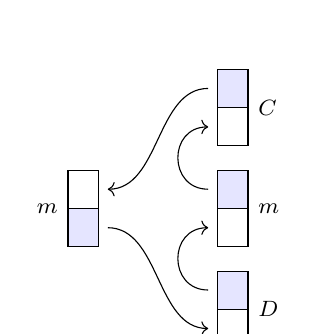
\begin{tikzpicture}[polybox, tos]
	\node[poly, dom, "$m$" left] (m) {};
	\node[poly, cod, right=of m, "$m$" right] (mm) {};
	\node[poly, cod, above=of mm, "$C$" right] (C) {};
	\node[poly, cod, below=of mm, "$D$" right] (D) {};
%
	\draw (m_pos) to[out=0, in=180] (D_pos);
	\draw (D_dir) to[climb] (mm_pos);
	\draw (mm_dir) to[climb] (C_pos);
	\draw (C_dir) to[last] (m_dir);
\end{tikzpicture}
}

\newcommand{\treepic}{
\begin{tikzpicture}[trees, scale=1.5,
  level 1/.style={sibling distance=20mm},
  level 2/.style={sibling distance=10mm},
  level 3/.style={sibling distance=5mm},
  level 4/.style={sibling distance=2.5mm},
  level 5/.style={sibling distance=1.25mm}]
  \node[dgreen] (a) {$\bullet$}
    child {node[dgreen] {$\bullet$}
    	child {node[dgreen] {$\bullet$}
    		child {node[dgreen] {$\bullet$}
  				child {node[dgreen] {$\bullet$}
    				child {}
    				child {}
    			}
  				child {node[dyellow] {$\bullet$}
    				child {}
    				child {}
    			}
  			}
    		child {node[dyellow] {$\bullet$}
					child {node[dgreen] {$\bullet$}
      			child {}
      			child {}
     			}
    			child  {node[red] {$\bullet$}}
  			}
    	}
    	child {node[dyellow] {$\bullet$}
    		child {node[dgreen] {$\bullet$}
  				child {node[dgreen] {$\bullet$}
    				child {}
    				child {}
    			}
  				child {node[dyellow] {$\bullet$}
    				child {}
    				child {}
    			}
  			}
    		child  {node[red] {$\bullet$}}
    	}
    }
    child {node[dyellow] {$\bullet$}
    	child {node[dgreen] {$\bullet$}
    		child {node[dgreen] {$\bullet$}
  				child {node[dgreen] {$\bullet$}
    				child {}
    				child {}
    			}
  				child {node[dyellow] {$\bullet$}
    				child {}
    				child {}
    			}
  			}
    		child {node[dyellow] {$\bullet$}
					child {node[dgreen] {$\bullet$}
      			child {}
      			child {}
     			}
    			child  {node[red] {$\bullet$}}
  			}
  		}
  		child {node[red] {$\bullet$}
  		}
  	}
  ;
\end{tikzpicture}
}

\newcommand{\coverpic}{
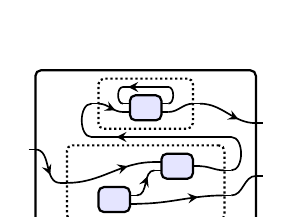
\begin{tikzpicture}[oriented WD, every fit/.style={inner xsep=\bbx, inner ysep=\bby}, bb small]
  \node[bb={2}{2}, fill=blue!10] (X1) {};
  \node[bb={1}{1}, fit={(X1) ($(X1.north)+(0,1)$)}, densely dotted] (Y1) {};
  \node[bb={2}{1}, fill=blue!10, below right=4 and 0 of X1] (X2) {};
  \node[bb={0}{2}, fill=blue!10, below left=of X2] (X3) {};
  \node[bb={1}{2}, fit=(X2) (X3), densely dotted] (Y2) {};
  \node[bb={1}{2}, fit=(Y1) (Y2)] (Z) {};
  \draw[ar] (Z_in1') to (Y2_in1);
  \draw[ar] (Y2_in1') to (X2_in1);
  \draw[ar] (X3_out1) to (X2_in2);
  \draw[ar] (X3_out2) to (Y2_out2');
  \draw (Y2_out2) to (Z_out2');
  \draw[ar] (Y1_in1') to (X1_in2);
  \draw (X1_out2) to (Y1_out1');
  \draw[ar] (Y1_out1) to (Z_out1');
  \draw (X2_out1) to (Y2_out1');
  \draw[ar] let \p1=(Y2.north east), \p2=(Y1.south west), \n1={\y1+\bby}, \n2=\bbportlen in
          (Y2_out1) to[in=0] (\x1+\n2,\n1) -- (\x2-\n2,\n1) to[out=180] (Y1_in1);
  \draw[ar] let \p1=(X1.north east), \p2=(X1.north west), \n1={\y1+\bby}, \n2=\bbportlen in
          (X1_out1) to[in=0] (\x1+\n2,\n1) -- (\x2-\n2,\n1) to[out=180] (X1_in1);
\end{tikzpicture}
}%{\earpic}
\tikzcdset{arrow style=tikz, diagrams={>=To}}

\tikzset{fit margins/.style={/tikz/afit/.cd,#1,
    /tikz/.cd,
    inner xsep=\pgfkeysvalueof{/tikz/afit/left}+\pgfkeysvalueof{/tikz/afit/right},
    inner ysep=\pgfkeysvalueof{/tikz/afit/top}+\pgfkeysvalueof{/tikz/afit/bottom},
    xshift=-\pgfkeysvalueof{/tikz/afit/left}+\pgfkeysvalueof{/tikz/afit/right},
    yshift=-\pgfkeysvalueof{/tikz/afit/bottom}+\pgfkeysvalueof{/tikz/afit/top}},
    afit/.cd,left/.initial=2pt,right/.initial=2pt,bottom/.initial=2pt,top/.initial=2pt}


\newcommand{\remarktitle}[1]{
    \par\vspace{\baselineskip}\noindent
    \textbf{\large #1}
    \par\noindent
}


%\DeclareUnicodeCharacter{2014}{\dash}

\usepackage{graphicx}								% Figures
\usepackage{subfig}									% Enables subfigures
\numberwithin{equation}{chapter}					% Numbering order for equations
\numberwithin{figure}{chapter}						% Numbering order for figures
\numberwithin{table}{chapter}						% Numbering order for tables
\usepackage{minted}						    		% Enables source code listings
\usepackage[top=3cm, bottom=3cm,
			inner=3cm, outer=3cm]{geometry}			% Page margin lengths			
\usepackage{eso-pic}								% Create cover page background
\newcommand{\backgroundpic}[3]{
	\put(#1,#2){
	\parbox[b][\paperheight]{\paperwidth}{
	\centering
	\includegraphics[width=\paperwidth,height=\paperheight,keepaspectratio]{#3}}}}
\usepackage{float} 									% Enables object position enforcement using [H]
\usepackage{parskip}								% Enables vertical spaces correctly 
\usepackage{datetime2} % date formatting tools - ISO-date YYYY-MM-DD
\usepackage{microtype} % Microtypography - improves readability and appearance of text.

% Allows clickable links for references, in table of content, autoref, etc.  	
\usepackage{hyperref}								
\hypersetup{colorlinks, citecolor=black,
   		 	filecolor=black, linkcolor=black,
    		urlcolor=black}

%% Bibliography https://www.overleaf.com/learn/latex/Bibliography_management_with_biblatex
\usepackage[style=ieee]{biblatex} % style=apa also possible
\addbibresource{references.bib}


% OPTIONAL SETTINGS (DELETE OR COMMENT TO SUPRESS)


		 

% Define the number of section levels to be included in the t.o.c. and numbered	(3 is default)	
\setcounter{tocdepth}{5}							
\setcounter{secnumdepth}{5}	


% Chapter title settings
\usepackage{titlesec}		
\titleformat{\chapter}[display]
  {\Huge\bfseries\filcenter}
  {{\fontsize{50pt}{1em}\vspace{-4.2ex}\selectfont \textnormal{\thechapter}}}{1ex}{}[]


% Header and footer settings (Select TWOSIDE or ONESIDE layout below)
\usepackage{fancyhdr}								
\pagestyle{fancy}  
\renewcommand{\chaptermark}[1]{\markboth{\thechapter.\space#1}{}} 


% Select one-sided (1) or two-sided (2) page numbering
\def\layout{2}	% Choose 1 for one-sided or 2 for two-sided layout
% Conditional expression based on the layout choice
\ifnum\layout=2	% Two-sided
    \fancyhf{}			 						
	\fancyhead[LE,RO]{\nouppercase{ \leftmark}}
	\fancyfoot[LE,RO]{\thepage}
	\fancypagestyle{plain}{			% Redefine the plain page style
	\fancyhf{}
	\renewcommand{\headrulewidth}{0pt} 		
	\fancyfoot[LE,RO]{\thepage}}	
\else			% One-sided  	
  	\fancyhf{}					
	\fancyhead[C]{\nouppercase{ \leftmark}}
	\fancyfoot[C]{\thepage}
\fi


% Enable To-do notes
\usepackage[textsize=tiny]{todonotes}   % Include the option "disable" to hide all notes
\setlength{\marginparwidth}{2.5cm} 


% Supress warning from Texmaker about headheight
\setlength{\headheight}{15pt}		




% Copied from https://github.com/armkeh/resume/blob/master/unicode-sty/unicode.sty

\usepackage{newunicodechar}


 % Our stuff
 
\newunicodechar{♯}{\ensuremath{\sharp}}
\newunicodechar{♭}{\ensuremath{\flat}}

\newunicodechar{∷}{::}
\newunicodechar{→}{$\rightarrow$}
\newunicodechar{∘}{$\circ$}
\newunicodechar{ₚ}{$_{\!\texttt{p}}$}
\newunicodechar{⊗}{$\otimes$}
\newunicodechar{≡}{$\equiv$}
\newunicodechar{≈}{$\approx$}
\newunicodechar{λ}{$\lambda$}
\newunicodechar{⊤}{$\top$}
\newunicodechar{⊥}{$\bot$}
\newunicodechar{⇆}{$\leftrightarrows$}
\newunicodechar{⇉}{$\rightrightarrows$}
\newunicodechar{⇒}{\ensuremath{\Rightarrow}}
\newunicodechar{ˡ}{\ensuremath{^{\!\texttt{l}}}}
\newunicodechar{ʳ}{\ensuremath{^{\!\texttt{r}}}}
\newunicodechar{∙}{\ensuremath{\bullet}}
\newunicodechar{²}{\ensuremath{^{\!2}}}
\newunicodechar{Σ}{\ensuremath{\Sigma}}
\newunicodechar{π}{\ensuremath{\pi}}
\newunicodechar{Π}{\ensuremath{\Pi}}
\newunicodechar{×}{\ensuremath{\times}}
\newunicodechar{◂}{\ensuremath{\triangleleft}}
\newunicodechar{⊎}{\ensuremath{\uplus}}
\newunicodechar{ᵀ}{\ensuremath{^{\!\texttt{T}}}}
\newunicodechar{⁻}{\ensuremath{^{-}}}
\newunicodechar{¹}{\ensuremath{^{1}}}
\newunicodechar{∀}{\ensuremath{\forall}}
\newunicodechar{η}{\ensuremath{\eta}}
\newunicodechar{⊣}{\ensuremath{\dashv}}
\newunicodechar{₁}{$_{\!1}$}
\newunicodechar{₂}{$_{\!2}$}
\newunicodechar{ℕ}{\ensuremath{\mathbb{N}}}
\newunicodechar{ℝ}{\ensuremath{\mathbb{R}}}
\newunicodechar{⟨}{\ensuremath{\langle}}
\newunicodechar{⟩}{\ensuremath{\rangle}}
\newunicodechar{σ}{\ensuremath{\sigma}}
\newunicodechar{ρ}{\ensuremath{\rho}}
\newunicodechar{β}{\ensuremath{\beta}}
\newunicodechar{γ}{\ensuremath{\gamma}}
\newunicodechar{δ}{\ensuremath{\delta}}
\newunicodechar{ₘ}{$_{\!\texttt{m}}$}
\newunicodechar{ₕ}{$_{\!\texttt{h}}$}
\newunicodechar{ₙ}{$_{\!\texttt{n}}$}
\newunicodechar{ˢ}{\ensuremath{^{\!\texttt{s}}}}



%---------------------------------------------------------------------
% Blackboard, calligraphic, etc.
%---------------------------------------------------------------------

%-----------------------------------------------------------
% Blackboard
%-----------------------------------------------------------

%-------------------------------------------------
% Lowercase latin
%-------------------------------------------------

\newunicodechar{𝕒}{\ensuremath{\mathbb{a}}}
\newunicodechar{𝕓}{\ensuremath{\mathbb{b}}}
\newunicodechar{𝕔}{\ensuremath{\mathbb{c}}}
\newunicodechar{𝕕}{\ensuremath{\mathbb{d}}}
\newunicodechar{𝕖}{\ensuremath{\mathbb{e}}}
\newunicodechar{𝕗}{\ensuremath{\mathbb{f}}}
\newunicodechar{𝕘}{\ensuremath{\mathbb{g}}}
\newunicodechar{𝕙}{\ensuremath{\mathbb{h}}}
\newunicodechar{𝕚}{\ensuremath{\mathbb{i}}}
\newunicodechar{𝕛}{\ensuremath{\mathbb{j}}}
\newunicodechar{𝕜}{\ensuremath{\mathbb{k}}}
\newunicodechar{𝕝}{\ensuremath{\mathbb{l}}}
\newunicodechar{𝕞}{\ensuremath{\mathbb{m}}}
\newunicodechar{𝕟}{\ensuremath{\mathbb{n}}}
\newunicodechar{𝕠}{\ensuremath{\mathbb{o}}}
\newunicodechar{𝕡}{\ensuremath{\mathbb{p}}}
\newunicodechar{𝕢}{\ensuremath{\mathbb{q}}}
\newunicodechar{𝕣}{\ensuremath{\mathbb{r}}}
\newunicodechar{𝕤}{\ensuremath{\mathbb{s}}}
\newunicodechar{𝕥}{\ensuremath{\mathbb{t}}}
\newunicodechar{𝕦}{\ensuremath{\mathbb{u}}}
\newunicodechar{𝕧}{\ensuremath{\mathbb{v}}}
\newunicodechar{𝕨}{\ensuremath{\mathbb{w}}}
\newunicodechar{𝕩}{\ensuremath{\mathbb{x}}}
\newunicodechar{𝕪}{\ensuremath{\mathbb{y}}}
\newunicodechar{𝕫}{\ensuremath{\mathbb{z}}}

%-------------------------------------------------
% Uppercase latin
%-------------------------------------------------

\newunicodechar{𝔸}{\ensuremath{\mathbb{A}}}
\newunicodechar{𝔹}{\ensuremath{\mathbb{B}}}
\newunicodechar{ℂ}{\ensuremath{\mathbb{C}}}
\newunicodechar{𝔻}{\ensuremath{\mathbb{D}}}
\newunicodechar{𝔼}{\ensuremath{\mathbb{E}}}
\newunicodechar{𝔽}{\ensuremath{\mathbb{F}}}
\newunicodechar{𝔾}{\ensuremath{\mathbb{G}}}
\newunicodechar{ℍ}{\ensuremath{\mathbb{H}}}
\newunicodechar{𝕀}{\ensuremath{\mathbb{I}}}
\newunicodechar{𝕁}{\ensuremath{\mathbb{J}}}
\newunicodechar{𝕂}{\ensuremath{\mathbb{K}}}
\newunicodechar{𝕃}{\ensuremath{\mathbb{L}}}
\newunicodechar{𝕄}{\ensuremath{\mathbb{M}}}
\newunicodechar{ℕ}{\ensuremath{\mathbb{N}}}
\newunicodechar{𝕆}{\ensuremath{\mathbb{O}}}
\newunicodechar{ℙ}{\ensuremath{\mathbb{P}}}
\newunicodechar{ℚ}{\ensuremath{\mathbb{Q}}}
\newunicodechar{ℝ}{\ensuremath{\mathbb{R}}}
\newunicodechar{𝕊}{\ensuremath{\mathbb{S}}}
\newunicodechar{𝕋}{\ensuremath{\mathbb{T}}}
\newunicodechar{𝕌}{\ensuremath{\mathbb{U}}}
\newunicodechar{𝕍}{\ensuremath{\mathbb{V}}}
\newunicodechar{𝕎}{\ensuremath{\mathbb{W}}}
\newunicodechar{𝕏}{\ensuremath{\mathbb{X}}}
\newunicodechar{𝕐}{\ensuremath{\mathbb{Y}}}
\newunicodechar{ℤ}{\ensuremath{\mathbb{Z}}}

%-------------------------------------------------
% Arabic numerals
%-------------------------------------------------

\newunicodechar{𝟙}{\ensuremath{\mathbb{1}}}
\newunicodechar{𝟚}{\ensuremath{\mathbb{2}}}
\newunicodechar{𝟛}{\ensuremath{\mathbb{3}}}
\newunicodechar{𝟜}{\ensuremath{\mathbb{4}}}
\newunicodechar{𝟝}{\ensuremath{\mathbb{5}}}
\newunicodechar{𝟞}{\ensuremath{\mathbb{6}}}
\newunicodechar{𝟟}{\ensuremath{\mathbb{7}}}
\newunicodechar{𝟠}{\ensuremath{\mathbb{8}}}
\newunicodechar{𝟡}{\ensuremath{\mathbb{9}}}
\newunicodechar{𝟘}{\ensuremath{\mathbb{0}}}

%-------------------------------------------------
% Greek
%-------------------------------------------------

\newunicodechar{ℾ}{\ensuremath{\mathbb{\Gamma}}}
\newunicodechar{ℽ}{\ensuremath{\mathbb{\gamma}}}
\newunicodechar{ℿ}{\ensuremath{\mathbb{\Pi}}}
\newunicodechar{ℼ}{\ensuremath{\mathbb{\pi}}}
\newunicodechar{⅀}{\ensuremath{\mathbb{\Sum}}}

%-----------------------------------------------------------
% Math calligraphic
%-----------------------------------------------------------

%-------------------------------------------------
% Uppercase latin
%-------------------------------------------------

\newunicodechar{𝒶}{\ensuremath{\mathcal{a}}}
\newunicodechar{𝒷}{\ensuremath{\mathcal{b}}}
\newunicodechar{𝒸}{\ensuremath{\mathcal{c}}}
\newunicodechar{𝒹}{\ensuremath{\mathcal{d}}}
\newunicodechar{ℯ}{\ensuremath{\mathcal{e}}}
\newunicodechar{𝒻}{\ensuremath{\mathcal{f}}}
\newunicodechar{ℊ}{\ensuremath{\mathcal{g}}}
\newunicodechar{𝒽}{\ensuremath{\mathcal{h}}}
\newunicodechar{𝒾}{\ensuremath{\mathcal{i}}}
\newunicodechar{𝒿}{\ensuremath{\mathcal{j}}}
\newunicodechar{𝓀}{\ensuremath{\mathcal{k}}}
\newunicodechar{𝓁}{\ensuremath{\mathcal{l}}}
\newunicodechar{𝓂}{\ensuremath{\mathcal{m}}}
\newunicodechar{𝓃}{\ensuremath{\mathcal{n}}}
\newunicodechar{ℴ}{\ensuremath{\mathcal{o}}}
\newunicodechar{𝓅}{\ensuremath{\mathcal{p}}}
\newunicodechar{𝓆}{\ensuremath{\mathcal{q}}}
\newunicodechar{𝓇}{\ensuremath{\mathcal{r}}}
\newunicodechar{𝓈}{\ensuremath{\mathcal{s}}}
\newunicodechar{𝓉}{\ensuremath{\mathcal{t}}}
\newunicodechar{𝓊}{\ensuremath{\mathcal{u}}}
\newunicodechar{𝓋}{\ensuremath{\mathcal{v}}}
\newunicodechar{𝓌}{\ensuremath{\mathcal{w}}}
\newunicodechar{𝓍}{\ensuremath{\mathcal{x}}}
\newunicodechar{𝓎}{\ensuremath{\mathcal{y}}}
\newunicodechar{𝓏}{\ensuremath{\mathcal{z}}}

%-------------------------------------------------
% Uppercase latin
%-------------------------------------------------

\newunicodechar{𝒜}{\ensuremath{\mathcal{A}}}
\newunicodechar{ℬ}{\ensuremath{\mathcal{B}}}
\newunicodechar{𝒞}{\ensuremath{\mathcal{C}}}
\newunicodechar{𝒟}{\ensuremath{\mathcal{D}}}
\newunicodechar{ℰ}{\ensuremath{\mathcal{E}}}
\newunicodechar{ℱ}{\ensuremath{\mathcal{F}}}
\newunicodechar{𝒢}{\ensuremath{\mathcal{G}}}
\newunicodechar{ℋ}{\ensuremath{\mathcal{H}}}
\newunicodechar{ℐ}{\ensuremath{\mathcal{I}}}
\newunicodechar{𝒥}{\ensuremath{\mathcal{J}}}
\newunicodechar{𝒦}{\ensuremath{\mathcal{K}}}
\newunicodechar{ℒ}{\ensuremath{\mathcal{L}}}
\newunicodechar{ℳ}{\ensuremath{\mathcal{M}}}
\newunicodechar{𝒩}{\ensuremath{\mathcal{N}}}
\newunicodechar{𝒪}{\ensuremath{\mathcal{O}}}
\newunicodechar{𝒫}{\ensuremath{\mathcal{P}}}
\newunicodechar{𝒬}{\ensuremath{\mathcal{Q}}}
\newunicodechar{ℛ}{\ensuremath{\mathcal{R}}}
\newunicodechar{𝒮}{\ensuremath{\mathcal{S}}}
\newunicodechar{𝒯}{\ensuremath{\mathcal{T}}}
\newunicodechar{𝒰}{\ensuremath{\mathcal{U}}}
\newunicodechar{𝒱}{\ensuremath{\mathcal{V}}}
\newunicodechar{𝒲}{\ensuremath{\mathcal{W}}}
\newunicodechar{𝒳}{\ensuremath{\mathcal{X}}}
\newunicodechar{𝒴}{\ensuremath{\mathcal{Y}}}
\newunicodechar{𝒵}{\ensuremath{\mathcal{Z}}}

\newunicodechar{ℓ}{\ensuremath{\ell}}

\newunicodechar{α}{\ensuremath{\alpha}}
\newunicodechar{Α}{\ensuremath{\Alpha}}
\newunicodechar{β}{\ensuremath{\beta}}
\newunicodechar{Β}{\ensuremath{\Beta}}
\newunicodechar{γ}{\ensuremath{\gamma}}
\newunicodechar{Γ}{\ensuremath{\Gamma}}
\newunicodechar{δ}{\ensuremath{\delta}}
\newunicodechar{Δ}{\ensuremath{\Delta}}
\newunicodechar{ϵ}{\ensuremath{\epsilon}}
\newunicodechar{Ε}{\ensuremath{\Epsilon}}
\newunicodechar{ζ}{\ensuremath{\zeta}}
\newunicodechar{Ζ}{\ensuremath{\Zeta}}
\newunicodechar{η}{\ensuremath{\eta}}
\newunicodechar{Η}{\ensuremath{\Eta}}
\newunicodechar{θ}{\ensuremath{\theta}}
\newunicodechar{Θ}{\ensuremath{\Theta}}
\newunicodechar{ι}{\ensuremath{\iota}}
\newunicodechar{Ι}{\ensuremath{\Iota}}
\newunicodechar{κ}{\ensuremath{\kappa}}
\newunicodechar{Κ}{\ensuremath{\Kappa}}
\newunicodechar{λ}{\ensuremath{\lambda}}
\newunicodechar{Λ}{\ensuremath{\Lambda}}
\newunicodechar{μ}{\ensuremath{\mu}}
\newunicodechar{Μ}{\ensuremath{\Mu}}
\newunicodechar{ν}{\ensuremath{\nu}}
\newunicodechar{Ν}{\ensuremath{\Nu}}
\newunicodechar{ξ}{\ensuremath{\xi}}
\newunicodechar{Ξ}{\ensuremath{\Xi}}
\newunicodechar{ο}{\ensuremath{\omicron}}
\newunicodechar{Ο}{\ensuremath{\Omicron}}
\newunicodechar{π}{\ensuremath{\pi}}
\newunicodechar{Π}{\ensuremath{\Pi}}
\newunicodechar{ρ}{\ensuremath{\rho}}
\newunicodechar{Ρ}{\ensuremath{\Rho}}
\newunicodechar{σ}{\ensuremath{\sigma}}
\newunicodechar{Σ}{\ensuremath{\Sigma}}
\newunicodechar{τ}{\ensuremath{\tau}}
\newunicodechar{Τ}{\ensuremath{\Tau}}
\newunicodechar{υ}{\ensuremath{\upsilon}}
\newunicodechar{Υ}{\ensuremath{\Upsilon}}
\newunicodechar{φ}{\ensuremath{\phi}}
\newunicodechar{Φ}{\ensuremath{\Phi}}
\newunicodechar{χ}{\ensuremath{\chi}}
\newunicodechar{Χ}{\ensuremath{\Chi}}
\newunicodechar{ψ}{\ensuremath{\psi}}
\newunicodechar{Ψ}{\ensuremath{\Psi}}
\newunicodechar{ω}{\ensuremath{\omega}}
\newunicodechar{Ω}{\ensuremath{\Omega}}

\newunicodechar{ε}{\ensuremath{\varepsilon}}
\newunicodechar{ϑ}{\ensuremath{\vartheta}}
\newunicodechar{ϰ}{\ensuremath{\varkappa}}
\newunicodechar{ϖ}{\ensuremath{\varpi}}
\newunicodechar{ς}{\ensuremath{\varsigma}}
\newunicodechar{φ}{\ensuremath{\varphi}}

\newunicodechar{ₐ}{\ensuremath{{}_{a}}}
\newunicodechar{ₑ}{\ensuremath{{}_{e}}}
\newunicodechar{ₕ}{\ensuremath{{}_{h}}}
\newunicodechar{ᵢ}{\ensuremath{{}_{i}}}
\newunicodechar{ⱼ}{\ensuremath{{}_{j}}}
\newunicodechar{ₖ}{\ensuremath{{}_{k}}}
\newunicodechar{ₗ}{\ensuremath{{}_{l}}}
\newunicodechar{ₘ}{\ensuremath{{}_{m}}}
\newunicodechar{ₙ}{\ensuremath{{}_{n}}}
\newunicodechar{ₒ}{\ensuremath{{}_{o}}}
\newunicodechar{ₚ}{\ensuremath{{}_{p}}}
\newunicodechar{ᵣ}{\ensuremath{{}_{r}}}
\newunicodechar{ₛ}{\ensuremath{{}_{s}}}
\newunicodechar{ₜ}{\ensuremath{{}_{t}}}
\newunicodechar{ᵤ}{\ensuremath{{}_{u}}}
\newunicodechar{ᵥ}{\ensuremath{{}_{v}}}
\newunicodechar{ₓ}{\ensuremath{{}_{x}}}

\newunicodechar{₀}{\ensuremath{{}_{0}}}
\newunicodechar{₁}{\ensuremath{{}_{1}}}
\newunicodechar{₂}{\ensuremath{{}_{2}}}
\newunicodechar{₃}{\ensuremath{{}_{3}}}
\newunicodechar{₄}{\ensuremath{{}_{4}}}
\newunicodechar{₅}{\ensuremath{{}_{5}}}
\newunicodechar{₆}{\ensuremath{{}_{6}}}
\newunicodechar{₇}{\ensuremath{{}_{7}}}
\newunicodechar{₈}{\ensuremath{{}_{8}}}
\newunicodechar{₉}{\ensuremath{{}_{9}}}

\newunicodechar{₊}{\ensuremath{{}_{+}}}

\newunicodechar{ᴬ}{\ensuremath{{}^{A}}}
\newunicodechar{ᴮ}{\ensuremath{{}^{B}}}
\newunicodechar{ᴰ}{\ensuremath{{}^{D}}}
\newunicodechar{ᴱ}{\ensuremath{{}^{E}}}
\newunicodechar{ᴳ}{\ensuremath{{}^{G}}}
\newunicodechar{ᴴ}{\ensuremath{{}^{H}}}
\newunicodechar{ᴵ}{\ensuremath{{}^{I}}}
\newunicodechar{ᴶ}{\ensuremath{{}^{J}}}
\newunicodechar{ᴷ}{\ensuremath{{}^{K}}}
\newunicodechar{ᴸ}{\ensuremath{{}^{L}}}
\newunicodechar{ᴹ}{\ensuremath{{}^{M}}}
\newunicodechar{ᴺ}{\ensuremath{{}^{N}}}
\newunicodechar{ᴼ}{\ensuremath{{}^{O}}}
\newunicodechar{ᴾ}{\ensuremath{{}^{P}}}
\newunicodechar{ᴿ}{\ensuremath{{}^{R}}}
\newunicodechar{ᵀ}{\ensuremath{{}^{T}}}
\newunicodechar{ᵁ}{\ensuremath{{}^{U}}}
\newunicodechar{ⱽ}{\ensuremath{{}^{V}}}
\newunicodechar{ᵂ}{\ensuremath{{}^{W}}}

\newunicodechar{ᵃ}{\ensuremath{{}^{a}}}
\newunicodechar{ᵇ}{\ensuremath{{}^{b}}}
\newunicodechar{ᶜ}{\ensuremath{{}^{c}}}
\newunicodechar{ᵈ}{\ensuremath{{}^{d}}}
\newunicodechar{ᵉ}{\ensuremath{{}^{e}}}
\newunicodechar{ᶠ}{\ensuremath{{}^{f}}}
\newunicodechar{ᵍ}{\ensuremath{{}^{g}}}
\newunicodechar{ʰ}{\ensuremath{{}^{h}}}
\newunicodechar{ⁱ}{\ensuremath{{}^{i}}}
\newunicodechar{ʲ}{\ensuremath{{}^{j}}}
\newunicodechar{ᵏ}{\ensuremath{{}^{k}}}
\newunicodechar{ˡ}{\ensuremath{{}^{l}}}
\newunicodechar{ᵐ}{\ensuremath{{}^{m}}}
\newunicodechar{ⁿ}{\ensuremath{{}^{n}}}
\newunicodechar{ᵒ}{\ensuremath{{}^{o}}}
\newunicodechar{ᵖ}{\ensuremath{{}^{p}}}
\newunicodechar{ʳ}{\ensuremath{{}^{r}}}
\newunicodechar{ˢ}{\ensuremath{{}^{s}}}
\newunicodechar{ᵗ}{\ensuremath{{}^{t}}}
\newunicodechar{ᵘ}{\ensuremath{{}^{u}}}
\newunicodechar{ᵛ}{\ensuremath{{}^{v}}}
\newunicodechar{ʷ}{\ensuremath{{}^{w}}}
\newunicodechar{ˣ}{\ensuremath{{}^{x}}}
\newunicodechar{ʸ}{\ensuremath{{}^{y}}}
\newunicodechar{ᶻ}{\ensuremath{{}^{z}}}

\newunicodechar{⁰}{\ensuremath{{}^{0}}}
\newunicodechar{¹}{\ensuremath{{}^{1}}}
\newunicodechar{²}{\ensuremath{{}^{2}}}
\newunicodechar{³}{\ensuremath{{}^{3}}}
\newunicodechar{⁴}{\ensuremath{{}^{4}}}
\newunicodechar{⁵}{\ensuremath{{}^{5}}}
\newunicodechar{⁶}{\ensuremath{{}^{6}}}
\newunicodechar{⁷}{\ensuremath{{}^{7}}}
\newunicodechar{⁸}{\ensuremath{{}^{8}}}
\newunicodechar{⁹}{\ensuremath{{}^{9}}}

\newunicodechar{⁺}{\ensuremath{{}^{+}}}

\newunicodechar{…}{\ensuremath{\ldots}}
\newunicodechar{⋯}{\ensuremath{\cdots}}
\newunicodechar{⋮}{\ensuremath{\vdots}}

\newunicodechar{–}{\ensuremath{\text{--}}}
\newunicodechar{—}{\ensuremath{\text{---}}}

\newunicodechar{⦅}{\ensuremath{(\!|}}
\newunicodechar{⦆}{\ensuremath{|\!)}}
\newunicodechar{⟨}{\ensuremath{\langle}}
\newunicodechar{⟩}{\ensuremath{\rangle}}
\newunicodechar{⟪}{\ensuremath{\langle\!\langle}}
\newunicodechar{⟫}{\ensuremath{\rangle\!\rangle}}
\newunicodechar{⁅}{\ensuremath{\{}}
\newunicodechar{⁆}{\ensuremath{\}}}
\newunicodechar{{}{\ensuremath{\{}}
\newunicodechar{}}{\ensuremath{\}}}

\newunicodechar{⌜}{\ensuremath{\ulcorner}}
\newunicodechar{⌝}{\ensuremath{\urcorner}}
\newunicodechar{⌞}{\ensuremath{\llcorner}}
\newunicodechar{⌟}{\ensuremath{\lrcorner}}
\newunicodechar{⌈}{\ensuremath{\lceil}}
\newunicodechar{⌉}{\ensuremath{\rceil}}
\newunicodechar{⌊}{\ensuremath{\lfloor}}
\newunicodechar{⌋}{\ensuremath{\rfloor}}

\newunicodechar{ }{\ensuremath{~}}

\newunicodechar{∀}{\ensuremath{\forall}}
\newunicodechar{∃}{\ensuremath{\exists}}

\newunicodechar{≡}{\ensuremath{\equiv}}
\newunicodechar{¬}{\ensuremath{\lnot}}
\newunicodechar{≢}{\ensuremath{\nequiv}}
\newunicodechar{∨}{\ensuremath{\lor}}
\newunicodechar{∧}{\ensuremath{\land}}
\newunicodechar{⇒}{\ensuremath{\;\Rightarrow\;}}
\newunicodechar{⇐}{\ensuremath{\;\Rightarrow\;}}
\newunicodechar{⇔}{\ensuremath{\iff}}

\newunicodechar{⊢}{\ensuremath{\vdash}}
\newunicodechar{⊣}{\ensuremath{\dashv}}
\newunicodechar{⊨}{\ensuremath{\vDash}}

\newunicodechar{ø}{\ensuremath{\emptyset}}
\newunicodechar{∅}{\ensuremath{\emptyset}}
\newunicodechar{∈}{\ensuremath{\in}}
\newunicodechar{∉}{\ensuremath{\not\in}}
\newunicodechar{∋}{\ensuremath{\ni}}
\newunicodechar{∩}{\ensuremath{\cap}}
\newunicodechar{∪}{\ensuremath{\cup}}
\newunicodechar{⊍}{\ensuremath{\uplus}}
\newunicodechar{⊎}{\ensuremath{\uplus}}

\newunicodechar{⊤}{\ensuremath{\top}}
\newunicodechar{⊥}{\ensuremath{\bot}}
\newunicodechar{⊔}{\ensuremath{\sqcup}}
\newunicodechar{⊓}{\ensuremath{\sqcap}}

\newunicodechar{∘}{\ensuremath{\circ}}

\newunicodechar{≠}{\ensuremath{\neq}}
\newunicodechar{≐}{\ensuremath{\doteq}}
\newunicodechar{≟}{\ensuremath{\stackrel{?}{=}}}
\newunicodechar{≅}{\ensuremath{\cong}}
\newunicodechar{≇}{\ensuremath{\ncong}}
\newunicodechar{≃}{\ensuremath{\simeq}}
\newunicodechar{≄}{\ensuremath{\nsimeq}}
\newunicodechar{≈}{\ensuremath{\approx}}
\newunicodechar{≉}{\ensuremath{\napprox}}
\newunicodechar{∼}{\ensuremath{\sim}}
\newunicodechar{≁}{\ensuremath{\nsim}}
\newunicodechar{≔}{\ensuremath{:\!=}}

\newunicodechar{≤}{\ensuremath{\leq}}
\newunicodechar{≰}{\ensuremath{\nleq}}
\newunicodechar{≥}{\ensuremath{\geq}}
\newunicodechar{≱}{\ensuremath{\ngeq}}
\newunicodechar{≮}{\ensuremath{\nless}}
\newunicodechar{≯}{\ensuremath{\ngtr}}
\newunicodechar{≦}{\ensuremath{\leqq}}
\newunicodechar{≨}{\ensuremath{\lneqq}}
\newunicodechar{≧}{\ensuremath{\geqq}}
\newunicodechar{≩}{\ensuremath{\gneqq}}
\newunicodechar{≲}{\ensuremath{\lesssim}}
\newunicodechar{≳}{\ensuremath{\gtrsim}}
\newunicodechar{⊏}{\ensuremath{\sqsubset}}
\newunicodechar{⊑}{\ensuremath{\sqsubseteq}}
\newunicodechar{⊐}{\ensuremath{\sqsupset}}
\newunicodechar{⊒}{\ensuremath{\sqsupseteq}}
\newunicodechar{∣}{\ensuremath{\mid}}

\newunicodechar{→}{\ensuremath{\rightarrow}}
\newunicodechar{←}{\ensuremath{\leftarrow}}
\newunicodechar{↑}{\ensuremath{\uparrow}}
\newunicodechar{↓}{\ensuremath{\downarrow}}
\newunicodechar{⟶}{\ensuremath{\longrightarrow}}
\newunicodechar{⟵}{\ensuremath{\longleftarrow}}

\newunicodechar{⊕}{\ensuremath{\oplus}}
\newunicodechar{⊖}{\ensuremath{\ominus}}
\newunicodechar{⊗}{\ensuremath{\otimes}}
\newunicodechar{⊘}{\ensuremath{\oslash}}
\newunicodechar{⊙}{\ensuremath{\odot}}
\newunicodechar{⊚}{\ensuremath{\circledcirc}}
\newunicodechar{⊛}{\ensuremath{\circledast}}
\newunicodechar{⊜}{\ensuremath{\circledequal}}
\newunicodechar{⊝}{\ensuremath{\circleddash}}

\newunicodechar{∶}{\ensuremath{\ratio}}
\newunicodechar{⨾}{\ensuremath{\fcmp}}

\newunicodechar{∙}{\ensuremath{\cdot}}
\newunicodechar{∞}{\ensuremath{\infty}}


\begin{document} 

\newcommand{\oneLineTitle}{Polynomial Functors in Agda: Theory and Practice}
\newcommand{\multiLineTitle}[1]{Polynomial Functors in Agda: \\[#1]  Theory and Practice}
% The term [#1] indicates that there will be 1 rowbreak to split the title into two pieces, first part before \\[#1] and second part after. If you have a very long title and need to split it up into 3 rows, just use \\[#1] multiple times.

\newcommand{\oneLineSubtitle}{A formalization and collection of applications of categories of polynomial functors}





% COVER PAGE, TITLE PAGE AND IMPRINT PAGE
\pagenumbering{roman}			% Roman numbering (starting with i (one)) until first main chapter
% CREATED BY DAVID FRISK, 2016
% MODIFIED BY JAKOB JARMAR, 2016
% A few changes by Birgit Grohe, 2017 and \the\year
% Adjustments with the help of Gustav Örtenberg 2019

% COVER PAGE
{ %% Scoped to not change parskip outside the titlepage


\begin{titlepage}
\newgeometry{top=3cm, bottom=3cm,
			left=2.25 cm, right=2.25cm}	% Temporarily change margins		
			
% Cover page background 
\AddToShipoutPicture*{\backgroundpic{-4}{56.7}{figure/auxiliary/frontpage_gu_eng_vec_m2.pdf}}
\addtolength{\voffset}{2cm}

% Cover picture (replace with your own or delete)		
\begin{figure}[H]
\centering
\vspace{1cm}	% Adjust vertical spacing here
%\includegraphics[width=0.9\linewidth]{figure/somepicture}
\end{figure}

% Cover text
\mbox{}
\vfill
\renewcommand{\familydefault}{\sfdefault} \normalfont % Set cover page font

\textbf{\Huge \multiLineTitle{0.2cm}} 
\\[0.5cm]

{\Large \oneLineSubtitle}\\[0.5cm]

%{\Large A Subtitle that can be Very Much Longer if Necessary}\\[0.5cm]

Master's thesis in Computer science and engineering \setlength{\parskip}{1cm}

{\Large Marcus Jörgensson} \setlength{\parskip}{2.9cm}
\\
\\
{\Large André Muricy Santos} \setlength{\parskip}{2.9cm}

Department of Computer Science and Engineering \\
\textsc{Chalmers University of Technology} \\
\textsc{University of Gothenburg} \\
Gothenburg, Sweden \the\year

\renewcommand{\familydefault}{\rmdefault} \normalfont % Reset standard font
\end{titlepage}


% BACK OF COVER PAGE (BLANK PAGE)
\newpage
\restoregeometry
\thispagestyle{empty}
\mbox{}


% TITLE PAGE
\newpage
\thispagestyle{empty}
\begin{center}
	\textsc{\large Master's thesis \the\year}\\[4cm]		% Report number is currently not in use
	\textbf{\Large \multiLineTitle{0.2cm}} \\[1cm]
	{\large \oneLineSubtitle}\\[1cm]
	{\large ANDRÉ MURICY SANTOS}
        {\large MARCUS JÖRGENSSON}
	
	\vfill	
	% Logotype on titlepage	
	\begin{figure}[H]
	\centering
	% Remove the following line to remove the titlepage logotype
	
\includegraphics[width=0.25\pdfpagewidth]{figure/auxiliary/ChGULogoHog.pdf}
	\end{figure}	\vspace{5mm}	
	
	Department of Computer Science and Engineering\\
	%\emph{Division of Division name}\\
	%Name of research group (if applicable)\\
	\textsc{Chalmers University of Technology} \\
	\textsc{University of Gothenburg} \\
	Gothenburg, Sweden \the\year \\
\end{center}


% IMPRINT PAGE (BACK OF TITLE PAGE)
\newpage
\thispagestyle{plain}
\vspace*{4.5cm}
\oneLineTitle\\
\oneLineSubtitle\\
ANDRÉ MURICY SANTOS \setlength{\parskip}{1cm},
MARCUS JÖRGENSSON \setlength{\parskip}{1cm}

\copyright ~ ANDRÉ MURICY SANTOS, \the\year. \setlength{\parskip}{1cm}
\copyright ~ MARCUS JÖRGENSSON, \the\year. \setlength{\parskip}{1cm}

Supervisor: Felix Cherubini, Logic and types\\
Examiner: Andreas Abel, Logic and types \setlength{\parskip}{1cm}

Master's Thesis \the\year\\	% Report number currently not in use 
Department of Computer Science and Engineering\\
%Division of Division name\\
%Name of research group (if applicable)\\
Chalmers University of Technology and University of Gothenburg\\
SE-412 96 Gothenburg\\
Telephone +46 31 772 1000 \setlength{\parskip}{0.5cm}

\vfill
% Caption for cover page figure if used, possibly with reference to further information in the report
% Cover: Description of the picture on the cover page (if applicable)


Typeset in \LaTeX \\
%Printed by [Name of printing company]\\
Gothenburg, Sweden \the\year

}

% % ABSTRACT
\newpage
% CREATED BY DAVID FRISK, 2016
%\oneLineTitle\\
%\oneLineSubtitle\\
%MARCUS JÖRGENSSON\\
%ANDRÉ MURICY SANTOS\\
%Department of Computer Science and Engineering\\
%Chalmers University of Technology and University of Gothenburg

\thispagestyle{plain}			% Supress header 
\section*{Abstract}

The category of polynomial functors - \textbf{Poly} - has been studied for over two decades and is well known for its relevance to computer science \cite{containersPaper} and deep mathematical structure \cite{polynomialFunctorsCategory}.
In recent years, Poly has found use in dynamical systems theory \cite{poly-book} \cite{css}. 
This thesis formalizes Poly and its use in dynamical systems in Cubical Agda, contributing to the Poly code ecosystem.
In the first part, the theory of the category Poly is formalized, together with a closely related category called Chart. 
In the second part, the use of Poly and Chart for building dynamical systems is given, together with many examples of dynamical systems.

The theory part formalizes the category Poly itself and several categorical constructs, including the initial object, products, composition and parallel product as two monoids, and many various proofs around the category.
Also, Chart is formalized, together with its own categorical constructs.
The combination of Poly and Chart as commuting squares is given, which is meaningful for the dynamical interpretation.

The practical part builds upon the theory by formalizing how these categories can be used to construct dynamical systems.
It covers how morphisms in Poly represent dynamical systems, how polynomials act as interfaces, how
systems are wired together, how systems are implemented, how behavior is installed into wiring diagrams, and how to run systems arriving at concrete programs.
Many dynamical system examples are given, such as the Fibonacci sequence generator, the Lorenz system, the Hodkgin-Huxley model, and reservoir computers.
Commuting squares are used as a way of showing that one dynamical system simulates another.



%to implement systems, how to install behavior into
%wiring diagrams, and how to run systems arriving at concrete programs.
%Special 

% Lenses
% between special polynomials have been shown to correspond to different concepts,
% such as DFA’s or Moore machines, which shows the power polynomials and lenses
% possess as an abstraction generalization. Some programs implemented are Fibonacci
% sequence generators, the Lorenz system, the Hodgkin-Huxley model, and reservoir
% computers. Combining theory and applications, commuting squares between lenses
% and charts have been used to show how one dynamical system can simulate another.


% Combination

%Talk about theory formalization.

%Talk about dynamical systems.




%heory of the c0ategory \textbf{Poly} 

%A formalization of the theory of the category \textbf{Poly} and a closesly related category \textbf{ by providing a formalization of the theory of the category \textbf{Poly} as well as a closely related category \textbf{Charts}, and showing how these categories can be used for dynamical systems.
%Many examples of d

%However, in recent years, researchers in the growing field of Applied Category Theory have found wider interpretations of the content of \textbf{Poly} and related topics, leading to applications in dynamical systems theory \cite{jaz http://davidjaz.com/Papers/DynamicalBook.pdf}, information theory \cite{https://arxiv.org/pdf/2201.12878.pdf}, database theory \cite{spivak db https://arxiv.org/pdf/2111.10968.pdf} and more. 
%Many aspects of the well-behavedness and richness of interpretation of \textbf{Poly} are being collected in the textbook \textit{Polynomial Functors - A Mathematical Theory of Interaction \cite{poly-book}}.


%However, the surrounding code ecosystem of \textbf{Poly} is lacking. It is difficult to find straightforward formalizations and/or programs that use \textbf{Poly}'s structure to their advantage. The present work seeks to contribute to this ecosystem by providing formalizations in Cubical Agda of many existing theorems and categorical constructs in \textbf{Poly} and closely related categories, along with an array of concrete examples of its application to real world, widely studied dynamical systems. Most of the code follows the aforementioned textbook as a general blueprint, but since the very authors admit to the youth of applied category theory as a field and specifically its perspective on \textbf{Poly}, we sometimes deviate and show new applications.

% KEYWORDS (MAXIMUM 10 WORDS)
\vfill
Keywords: Category theory, Dependent types, Agda, Cubical, Polynomial functors, Dynamical systems, Complex systems

\newpage				% Create empty back of side
\thispagestyle{empty}
\mbox{}

% % ACKNOWLEDGEMENTS
\newpage
% CREATED BY DAVID FRISK, 2016
\thispagestyle{plain}			% Supress header
\section*{Acknowledgements}
Firstly, we would like to acknowledge and thank Naïm Camille Favier for the help via the Agda Zulip in several proofs: solving a problem with characterizing lens equality, making the inclusion map in set coequalizers type-check, and for general guidance in Agda-related questions.

%helping formulate the isomorphism of comonoids in \textbf{Poly} and small categories, 

Secondly, we would like to acknowledge David Orion Girardo for his succinct and beautiful formulation of the composition operator we used, and for inspiration in Agda.


Thirdly, we thank David Spivak, co-author of the textbook we follow for this thesis and many of the papers we cite. We could not have done it without his and Nelson Niu's wonderful book. Or without his warm encouragement to pursue this project.

Fourth, André would like to thank Daniel Satanove, whose tutoring proved vital in understanding some of the more advanced categorical ideas.

Finally, we thank our supervisor Felix Cherubini, whose patience, guidance, and expertise were instrumental in bringing this thesis to life.

%\vspace{1.5cm}
%\hfill
%André Muricy Santos, Gothenburg, \today
%Marcus Jörgensson, Gothenburg, \today

\newpage				% Create empty back of side
\thispagestyle{empty}
\mbox{}


% TABLE OF CONTENTS
\newpage
\setcounter{tocdepth}{2}
\tableofcontents

% OTHER FRONTMATTER
% List of figures (add to table of contents)
%\cleardoublepage
%\addcontentsline{toc}{chapter}{\listfigurename} 
%\listoffigures
% List of tables (add to table of contents)
%\cleardoublepage
%\addcontentsline{toc}{chapter}{\listtablename}  
%\listoftables


% START OF MAIN DOCUMENT
\cleardoublepage
\setcounter{page}{1}
\pagenumbering{arabic}			% Arabic numbering starting from 1 (one)


% INTRODUCTION
% CREATED BY DAVID FRISK, 2016
\chapter{Introduction}
Category theory is an area of mathematics concerned with abstraction and mathematical structure. The category of polynomial functors, named \textbf{Poly}, has been studied for over two decades. \textbf{Poly}\footnote{\textbf{Poly} is also known as the category of containers.} is known for its relevance to computer science, as well as for its deep mathematical structure. In recent years, researchers in the emerging field of applied category theory have found interpretations of \textbf{Poly} in several fields of science and engineering, including dynamical systems theory. The purpose of this thesis is to contribute to the code ecosystem of \textbf{Poly} and its use in dynamical systems.


%In complex systems theory, it is of interest to find a level of abstraction that brings out commonalities between different systems. Sometimes, unrelated systems might reveal themselves to have some deep structural similarity. However, arriving at a fundamental mathematical theory of complex systems is difficult. 

%Category theory is an area of mathematics that is concerned with abstraction and finding common concepts between different branches of mathematics. The power of category theory has been used in type theory and programming language theory for many decades and is now finding its  applications in scientific fields.  


%Recently, the book "Polynomial Functors: A Mathematical Theory of Interaction" was written, hereafter referred to as the poly-book. It However, laou.

%The goal of this thesis is to contribute to this 
%there is concern of finding the right level of abstraction, to seek commonalities between systems. 


%Do funneling. Short and easy, last sentence should be purpose of report.

\section{Applied category theory and complex systems}
In the study of complex systems, there is a concern of finding the right level of abstraction at which to seek commonalities between different systems. Sometimes, seemingly unrelated systems might reveal themselves to have some deep structural similarity, like critical transitions in ecosystems \cite{catastrophic}. However, arriving at a fundamental mathematical theory of complex systems is profoundly difficult. The immense expressive power of category theory has been a staple of type theory and programming language theory for many decades, and this robust mathematical language is now finding its footing in expressing ideas from wider scientific fields as well, including fields under the umbrella of complex systems. Some of the applications include foundations of complex systems \cite{complexcatsadjunction}, game theory \cite{compositional-gt}, probability \cite{markov-categories}, systems biology \cite{compositional-react-net} and dynamical systems theory \cite{operad-dynsys}.

\remarktitle{Polynomial functors and dynamical systems}
In particular, \textbf{Poly} turns out to be useful in the modeling of so-called mode-dependent open dynamical systems. The "open" part of this class of systems refers to the fact that they not only have an internal dynamics and state space, but can interact with their environment by accepting external inputs and providing external outputs. The "mode-dependent" part refers to the fact that this paradigm of interaction \textit{can change} depending on the internal state of the system, meaning they can, throughout time, accept inputs and provide outputs to different environments.

This is a remarkably general form of system which \textbf{Poly} fully embeds in the categorical context, which implies that questions like "what does it mean to take the product of two systems?" often have a concrete and intuitive meaning for the dynamics of the resulting system.

\section{The \textit{poly-book}}
Many aspects of the behavior and richness of \textbf{Poly} are collected in a newly written (still in draft at the time of writing this thesis) textbook, \textit{Polynomial Functors: A Mathematical Theory of Interaction}, hereafter called the poly-book. The book is being written by David Spivak and Nelson Niu and consists of a deep dive into \textbf{Poly}, explaining its mathematical structure in detail as well as providing many practical consequences of this structure to modeling dynamical systems. The authors also gave a course based on the book, and the lectures are freely available on YouTube. In this lecture series, some categories closely related to \textbf{Poly} are explored, which hint at an even bigger potential for application.


\section{Goal of this thesis}
We believe that the surrounding ecosystem of \textbf{Poly} is lacking. It is difficult to find straightforward formalizations of the category, or programs/dynamical systems models that use its structure to their advantage. The goal of this thesis is to advance this ecosystem. We follow the poly-book and its associated lecture series as a blueprint, and rely on the explanations therein to contribute several categorical formalizations, as well as show how \textbf{Poly} can be used to model different examples of dynamical systems by providing implementations. Some of these examples are described informally in the poly-book, others we come up with. We do not aim to formalize all theorems or implement all the examples in the book, as this would be simply too much work for this thesis. Instead, we constrain ourselves to what we deem the most essential constructs and illustrative examples.
% The intro is under reconstruction :) And the abstract will be reconstructed to be more of an abstract as well.


% Formalization of Poly in Agda. Prove many theorems and categorical constructs of Poly, and the related category of charts. 
% Many well known dynamical systems as examples.  
% Will follow the poly book as blueprint.

% \section{Delimitations}

% Not everything from the poly-book will be proved. Guideline. The proof of theorems might differ, one reason being that 
% Can write about some delimations, some differentiation

\section{Outline}
The outline of the thesis is as follows; first, some of the needed background is explained in chapter \ref{chapter:background}. Then, the theoretical part of the thesis is given, formalizing two categories of polynomial functors and their categorical constructs. The primary category, of lenses, is given in chapter \ref{chapter:lenses} and charts in chapter \ref{chapter:charts}. Chapter \ref{chapter:application} consists of the practice part of the thesis, how \textbf{Poly} is used for dynamical systems, together with several examples. After, in chapter \ref{chapter:discussion}, a discussion of the formalization is given, as well as future work. Finally, in chapter \ref{chapter:conclusion}, conclusions are drawn about how well the result of the thesis met its purpose.

All the code for this formalization is freely available on GitHub \footnote{\href{https://github.com/amuricys/polynomial-functors/}{https://github.com/amuricys/polynomial-functors/}}.

% Purpose: Formalize categoriy theory of Poly. Showing how dynamical systems can be implemented using poly.



%We see the poly-book another contribution to this landscape, as well as to category theory at large. It is a proper deep dive on \textbf{Poly}, and frequently oscillates between explaining the mathematical structure of the category and providing interpretations of it in real-world contexts. 


%Like the book, this thesis is perhaps unusual in the sense that, as the title suggests, it is equally concerned with the extremely abstract side of thinking about \textbf{Poly} (the \textit{Theory} part of the subtitle), as well as with the extremely concrete and mundane side of it (the \textit{Applications} part). 
%In this sense, we straddle a line between two extremes. This divide is exhibited clearly in the style of code that pertains to each part, and by the style of reasoning required to understand and appreciate each one. One might find oneself mentally "juggling" very different cognitive contexts if the change between the two subjects happens too frequently, and so we prefer to make this split explicit upfront, to the extent that we can, and reflect it in the structure of the writing itself by having two parts. This also has the benefit of being a more faithful representation of how the work was actually done: many evenings were spent struggling with only attempting to formalize categorical concepts, and many others with struggling to tune dynamical systems parameters to get the right behavior and plots. Of course, when theory is directly relevant to our example applications, we pay it due mention, but that is more the exception than the rule.

%This divide is not meant to be taken too literally: some of our applications are to fields that have their own rich theories to which lifetimes of study could be dedicated, like neuromorphic computing and reservoir computers, and some of the applications "loop back" into the theory of \textbf{Poly} itself, it is merely meant as a reflection of the two general fronts in which we're using and thinking about \textbf{Poly}.

%Another aspect of the work is that \textbf{Poly} is not the only category with polynomial functors as objects. There is also the category of so-called \textit{charts} on polynomials, a different kind of morphism. It turns out that these two kinds of morphisms gives rise to an even richer, double category. We do some work on charts and their associated formalisms, and recover some direct applications of these formalisms, mostly based on David Jaz Myers' work. The main focus of the thesis, however, is the category \textbf{Poly}.




% THEORY
% CREATED BY DAVID FRISK, 2016
\chapter{Background}\label{chapter:background}
This chapter gives a short introduction to the technology used, as well as the different areas of knowledge needed to understand this thesis. For the technology, \textbf{Agda} and \textbf{Cubical Agda} are explained, as they provide the framework for the implementation. For the theory, a brief explanation of \textbf{Category Theory} is given, as well as some references to previous work on the main category of this thesis, \textbf{Poly}. Introducing the concepts of \textbf{Poly} is done in the theory section.

Some topics are not introduced in the background but at the point where they are used. There are also many citations and references to deeper explorations of most concepts mentioned.

%and the different areas of knowledge used within the thesis. It explains \textbf{Agda} and \textbf{Cubical Agda} which provides the framework for the implementation. It also explains what \textbf{Category Theory} is, and finally giving some context of the main category of this thesis, \textbf{Poly}.


% This chapter gives a short introduction to the technology used and different areas of knowledge that is needed to understand this thesis. Starting with explaining \textbf{Agda}, which is the programming language used for the formalization. Going on to \textbf{Cubical Agda} which is an extension to \textbf{Agda} providing useful constructs aiding in writing proofs. Then to \textbf{Category Theory}


% This chapter explains any background needed to understand this thesis. 

% the decisions made prior to starting the work - namely what technology to use, why, and what to use it for. We will also dedicate a brief effort to explaining the basics of category theory and its mechanisms for generalizing and illuminating the subjects it's applied to. Finally, we'll briefly explore the specific category of polynomial functors - \textbf{Poly}, its surprising amount of structure and numerous interpretations in many different contexts - in other words, we will explain why this work was done and why we believe \textbf{Poly}, and polynomial functors in general, to be important.

\section{Agda}
Agda is a dependently typed programming language \cite{agdaWebsite} created at Chalmers.
It is a functional language with very similar syntax to Haskell, but with a more powerful type system that allows it to be used as a proof assistant. 
Dependent types mean that types can depend on values. For example, a function have have the type signature \mintinline{agda}{natOrBool : (b : Bool) → if b then ℕ else Bool}, which means it returns a natural number if the value of the argument is true and a boolean if the value of the argument is false. In a non-dependent language, this would need to be expressed at the value level, so the function would have to return a value of type \mintinline{haskell}{Either ℕ Bool}.

\subsection{Unicode characters}
Agda, compared to most other languages, allows and makes heavy use of Unicode characters in symbol names. This can look daunting but provides for a concise syntax akin to mathematical notation. 

\subsection{Propositions as Types}
The Curry-Howard isomorphism \cite{propositionastypes} is the idea that there is a one-to-one correspondence between types in programming languages, propositions in logic, and expressions in algebra. Under this correspondence (isomorphism), a value of a type can be seen as a proof of the proposition the type corresponds to \cite{DependentTypesAtWork}. For example, the following data type in Agda corresponds to the logical operator \texttt{or} (written $A \vee B$):

\begin{minted}{agda}
data Either (A B : Type) : Set where
    inj₁ : A → Either A B
    inj₂ : B → Either A B
\end{minted}

Concretely, an element of type \texttt{Either A B} is either an element of \texttt{A}, contained in the first value constructor \texttt{inj₁}, or of the type \texttt{B}, contained in the second value constructor \texttt{inj₂}. This corresponds to the fact that that a proof of the logical proposition $A \vee B$ is either a proof of the proposition \texttt{A} or a proof of \texttt{B}. This, in turn, also corresponds to summing in algebra - $A + B$. A summary of the isomorphism is given below:

\begin{table}[H]
\begin{tabular}{lll}
Algebra      & Logic                   & Types \\
$A + B$      & $A \vee B$              & \texttt{Either A B} \\
$A \times B$ & $A \wedge B$            & \texttt{Pair A B}\\
$B^A$        & $ A \implies B$         & \texttt{A -> B} \\
$A = B$      & $ A \iff B$             & \texttt{Iso A B}\\
$0$          & $ false $               & \texttt{⊥}\\
$1$          & $ true  $               & \texttt{⊤}
\end{tabular}
\end{table}


The Curry-Howard isomorphism and Agda's powerful type system make Agda a powerful proof checker.


\subsection{Agda examples}
The \mintinline{agda}{Either} example above shows how (polymorphic) datatypes are defined, similar to the GADTs \cite{haskellGADT} extension of Haskell.

It is also possible to create record types for data types with only one constructor.

\begin{minted}{agda}
record Action : Type where
  constructor mkAction
  field
    write : Alphabet
    move : Movement
\end{minted}

The unit type and unit function are defined as:
\begin{minted}{agda}
data ⊤ : Type where
    tt : ⊤

unit : {A : Type} → A → ⊤
unit _ = tt
\end{minted}

The bottom (or False) type and the absurd function from bottom:
\begin{minted}{agda}
data ⊥ : Type where

absurd : {A : Type} → ⊥ → A
absurd ()
\end{minted}

The \texttt{natOrBool} function can be implemented as:
\begin{minted}{agda}
natOrBool : (b : Bool) → if b then ℕ else Bool
natOrBool true = 0
natOrBool false = true
\end{minted}

More explanations and examples of Agda can be found in \cite{agdaWebsite} and \cite{DependentTypesAtWork}. Otherwise, it should be possible to understand the more advanced concepts of Agda along the thesis.

\subsection{Foreign function interface - Haskell}
Agda has a fully-featured foreign function interface (FFI) with Haskell, providing access to the vast Haskell ecosystem. The FFI is important to the application section, to use well-established libraries for plotting graphs, writing versatile command-line interfaces, and fast matrix inversion. For a more detailed description of the supporting Haskell code and its use, see appendix \ref{app:haskell}.


%The programming language Agda is a natural choice for this project. Dependently typed programming languages allow for the expression of an incredibly vast array of mathematical concepts with the appropriate rigor, and Agda is a mature and robust language in this space. 

%It also has a fully-featured FFI to work with its compilation target, Haskell. This is important to our application work, where we sometimes need to use the Haskell ecosystem to produce things like plots and graphs and use BLAS-based matrix multiplication algorithms. 

% Further, Agda is developed within Chalmers, which allows us access to a great deal of expertise in the details of the language within the University.

\section{Cubical Agda}
Cubical \cite{cubicalAgdaDocs} is an extension of Agda, bringing ideas from Homotopy Type Theory (HoTT) \cite{hottBook}. The main contribution of Cubical Agda is how to deal with equality.

Normal Agda defines equality as a data type. However, this (propositional) equality has certain problems. For example, it is not possible to prove function extensionality, that two functions are equal if they are equal for all arguments. Functional extensionality, which is very useful, is directly provable in Cubical.

Cubical discards this datatype and uses its own notion of equality, the path. An equality between elements $a : A$ and $b : A$ is a path from $a$ to $b$.
Cubical achieves this with a function $p : I \rightarrow A$ satisfying some conditions. Firstly, $I$ is a special kind of variable representing an interval or a path ranging from $0$ to $1$. It can be thougth of as a type representing an interval, although it isn't a type. Secondly, the beginning of the path must be $a$, that is $p(0)=a$. Finally, the end of the path must be $b$, $p(1)=b$. The important thing to note is that given \mintinline{agda}{a b : A} a type \mintinline{agda}{a ≡ b} is a function \mintinline{agda}{I → A} behind the scenes, satisfying the above conditions. 

The equality \mintinline{agda}{a ≡ b} is known as homogeneous equality because $a$ and $b$ have the same type. It is also possible to have an equality when $a$ and $b$ are of different types, named heterogeneous equality. Homogeneous equality is a special case of heterogeneous equality, where $a$ and $b$ have the same type. For this thesis, mostly equality between elements of a fixed type is used, so no further explanation of heterogeneous equality is needed.

It is also possible to combine Cubical Agda with propositional equality. Using the functions \mintinline{agda}{pathToEq} and \mintinline{agda}{eqToPath}, it is possible to go back and forth between the two different notions of equality, which is useful in some cases.

There exists a standard Cubical library \cite{cubicalLibrary} that has plenty of constructs and proofs from HoTT. The Cubical library is extensively used in this project.

A useful property of Cubical Agda is that the type of isomorphisms is the same as the type of equalities. It is possible to go back and forth using \mintinline{agda}{isoToPath} and \mintinline{agda}{pathToIso}, from the standard Cubical library. This means that one way to prove an equality is to prove an isomorphism.

A final property, which is used heftily in this thesis, is substitution. Substitution makes it possible to transfer a property over an equality. The declaration of substitution, somewhat simplified, is 

\begin{minted}{agda}
subst : {A : Type} {x y : A} {B : A → Type} → (x ≡ y) → B x → B y
\end{minted}

The next subsection gives some more examples of Cubical Agda. Further information about Cubical Agda and HoTT can be found in  \cite{cubicalPaper} and \cite{hottBook}.

\subsection{Cubical examples}
The first example is to show that the absurd function, defined before, is unique. Given any other function from the empty type, it is the same function as absurd. Function extensionality is used to prove an equality between functions. Finally, the lemma is easily proved by pattern matching on the empty type.

\begin{minted}{agda}
absurdUnique : {A : Type} → (f : ⊥ → A) → f ≡ absurd
absurdUnique f = funExt lemma
    where
        lemma : (x : ⊥) → f x ≡ absurd x
        lemma ()
\end{minted}

In propositional equality, \mintinline{agda}{refl} is the constructor of the inductive data type representing equality, which provides a way to prove that any element $a$, is equal to itself. In Cubical, the function \mintinline{agda}{refl} is used instead. This function satisfies the requirement of being $a$ at both endpoints of the interval since it is constantly $a$. 

\begin{minted}{agda}
refl : {A : Type} → {a : A} → a ≡ a
refl {a = a} i = a
\end{minted}


% Cubical Type Theory \cite{cubical} is a setting in which the Univalence Axiom from Homotopy Type Theory is computable. In Agda, this allows certain constructs to be defined more directly and for the expression of their properties to be much simplified. An example of this is set quotients - Dependent Martin-Löf Type Theory tends to avoid set quotients to instead rely on setoids. However, to express notions like set coequalizers cleanly, one needs quotients, and Cubical Agda allows them to be simply definable as Higher Inductive Types - HITs.

% Another major benefit to our work that Cubical Agda provides is that function extensionality is provable in HoTT. Since we are working on categorical formalizations, we constantly want to prove equalities of arrows in \textbf{Poly}, a problem that will turn out to be proving equalities of dependent and non-dependent functions.

% Yet another benefit is that doing Category Theory in a HoTT setting is just \textit{nice}. In Category Theory, mathematicians are often careful to distinguish strict equality from isomorphism, but in HoTT this distinction conveniently vanishes. We make extensive use of this fact via the function \textit{isoToPath} from the Cubical library. The HoTT book goes in more detail on how to do a constructive category theory in the context of HoTT, and this talk https://www.youtube.com/watch?v=nalC40POVLU by David Jaz Myers, author of one of the main references of this thesis \cite{css}, explains in a more relaxed fashion as well. 

% There's also no loss of expressivity, since the Cubical library allows to convert back and forth between cubical and propositional equality via the functions \textit{pathToEq} and \textit{eqToPath}; another tool we use frequently.

% Finally, our supervisor Felix Cherubini is an experienced homotopy type theorist, on whose expertise we're happy to have been able to rely.

\section{Category Theory}
Category theory (CT) is used heavily in this thesis. CT is the formal study of composition, building larger relationships from smaller ones. Its central objects of study are categories, where a category consists of some data and satisfies some laws. The most well-known category in computer science is the category of types and functions, but in this thesis, other categories are explored. 

%We make use of CT in this project in three different regards: we sometimes need to think about category theory in general and what is true in a pure context, sometimes how to apply categorical concepts to concrete scientific and engineering contexts, and sometimes on the syntactic issue of how to translate statements about CT to statements in Agda and its type theories. We will briefly expand on these three regards now.

% \subsection{In general: pure and applied CT}

%We think of Category Theory as the formal study of composition - meaning connecting two relationships to form a larger one. It has some axioms that always hold for its central object of study, which is categories themselves, and definitions that build on top of these axioms that allow a highly rigorous but simple form of abstract reasoning about either structures that exist within categories or between them. 

%The definitions and associated axioms are extremely simple; a \textit{category} $\mathcal{C}$ consists of the following data:
A \textit{category} $\mathcal{C}$ consists of the following data:

\begin{enumerate}
  \item A collection of objects Ob($\mathcal{C}$).
  \item For every two objects $A$ and $B$, a set of \textit{arrows} (also called \textit{morphisms} or \textit{maps}) between them denoted by $\mathcal{C}$(A , B). Individual arrows, are written like: $f : A \rightarrow B $.
  \item For every object $A$, an identity arrow $id : A \rightarrow A$. 
  \item A composition operator $ \circ $ , that gives rise to new arrows. For any three objects $A$, $B$ and $C$ and arrows $f : A \rightarrow B $ and $g : B \rightarrow C $, there exists an arrow $g \circ f : A \rightarrow C $.
\end{enumerate}

A category must fulfill the identity and assocativaity laws:

\begin{enumerate}
  \item $ \forall f. f \circ id = id \circ f = f $ (identity)
  \item $ \forall f\text{ }g\text{ }h. f \circ (g \circ h) = (f \circ g) \circ h $ (associativity of composition)
\end{enumerate}

\subsection{Commuting diagrams}
The usual way of representing statements in category theory is through \textit{commuting diagrams}. Such as:

 % https://q.uiver.app/?q=WzAsNCxbMCwxLCJBIl0sWzIsMSwiQyJdLFsxLDIsIkIiXSxbMSwwLCJEIl0sWzAsMiwiZiJdLFsyLDEsImciXSxbMCwzLCJoIl0sWzMsMSwiayJdXQ==
 % https://q.uiver.app/#q=WzAsNCxbMCwxLCJBIl0sWzIsMSwiQyJdLFsxLDIsIkIiXSxbMSwwLCJEIl0sWzAsMiwiZiJdLFsyLDEsImciXSxbMCwzLCJoIl0sWzMsMSwiayJdXQ==
\[\begin{tikzcd}
	& D \\
	A && C \\
	& B
	\arrow["f", from=2-1, to=3-2]
	\arrow["g", from=3-2, to=2-3]
	\arrow["h", from=2-1, to=1-2]
	\arrow["k", from=1-2, to=2-3]
\end{tikzcd}\]
%  \begin{tikzcd}
%  	& D \\
%  	A && C \\
%  	& B
%  	\arrow["f", from=2-1, to=3-2]
%  	\arrow["g", from=3-2, to=2-3]
%  	\arrow["h", from=2-1, to=1-2]
%  	\arrow["k", from=1-2, to=2-3]
%  \end{tikzcd}

Here, the objects are $ A $, $ B $, $ C $ and $ D $, and the arrows are $ f : A \rightarrow B $, $ g : B \rightarrow C $, $ h : A \rightarrow D $ and $ k : D \rightarrow C $. Composite arrows and identity arrows are usually omitted from the diagram but are always there implicitly. \textit{Commuting} means that any path between two objects is the same; for this example $ k \circ h = g \circ f $. In a sense, diagrams can be seen as category theory's analog of abstract algebraic equations. Like equations handle symbols that can stand for anything, diagrams are an abstract representation of some structure in a category, containing objects and morphisms labeled and subject to constraints like being equal or unique, and should be interpreted as a statement.

% They must also respect the laws to be categories of course. In our case, because the thesis has a large focus on applied category theory, we will also talk frequently about the meaning of the arrows and objects in \textbf{Poly} and some closely related categories; it's what makes them interesting after all.

\subsection{Applied category theory}
In general settings of category theory, the meaning of the objects and arrows doesn't play any role - they are purposefully abstract. Concrete categories ought to have meaning to their arrows and what it means to compose them, like the category \textbf{Set}, where objects are sets and arrows are functions between them. Since this thesis has a large focus on applied category theory, there is always meaning of the arrows and objects in \textbf{Poly} and some closely related categories; it's what makes them interesting, after all.

Although the definition of a category may not seem like much, it, reveals \textit{the point} of category theory: it is a theory of \textit{compositionality}. What it means to compose relationships between objects, what facts are preserved under different compositions, how composing can generalize: this and other deep structural questions are at the core of this theory. 

In this spirit of investigating compositionality, \textit{applied} category theory is done. The main introductory textbook on the subject, \textit{Seven Sketches in Compositionality} \cite{seven-sketches}, does a good job of justifying this approach. The book usually starts with motivating examples in the real world and what CT and its constructions and formalisms can bring to understanding them in better, or at least different ways. For this thesis, the order is reversed; the theory is covered first, but the goal of applying is always present.

There are many constructions and structures in CT which would not be feasible to explain in this section. Instead, they are introduced as they become relevant.


%Defining the main point of study of category theory is barely scratching the surface. 

%There are many constructions and structures within the theory that we cannot explain in any detail that would do them justice here; instead we will introduce other concepts in CT as they become relevant.



\subsection{In code: Agda's \texttt{agda-categories} library}

The poly-book demonstrates many category-theoretic constructs in the context of \textbf{Poly}, but this thesis is limited to the most essential ones. These tend to be quite ubiquitous, and as such, there are formulations of many of them in the Agda ecosystem: the three main ones are the 1lab \cite{1lab}, the Cubical library's own \cite{cubical-cat}, and the \texttt{agda-categories} \cite{agda-cats} library. For this thesis, the third one is picked for a few reasons: firstly, it is very well documented, with a sensible user interface and active community. Secondly, it has more constructs: for example, it is the only one of the three in which the exponential object, a key feature of \textbf{Poly}, is present. Thirdly, it is interoperable with Cubical, since the definition of a category requires a user to provide an equivalence relation to express equality between arrows, where cubical equality can be supplied.
%\texttt{Agda-categories} provides a general scaffolidng making sure the formalizations of the categorical concepts in \textbf{Poly} are correct. % Sometimes, it also helps by providing pre-existing implementations of categories; for instance, polynomials are functors, and so we will often rely on the provided instance of the category of \textbf{Set} of sets and functions.

\section{Polynomial Functors}

The study of polynomial functors has an extensive literature in the pure category-theoretic setting, like the work of Joachim Kock \cite{kockpoly} \cite{kock2009polynomial}. In contrast, the \textbf{poly-book}, the main book of this thesis, is focused on applied category theory, providing interpretations of abstract mathematical structures that correspond, mapping them to concrete concepts and applications. Some of the most mature interpretations are database theory, decision systems, and dynamical systems. One of the book's authors, David Spivak, has done work using \textbf{Poly} in the context of database theory \cite{spivak2023functorial}. The book also spends some time developing intuitions on the decision-making perspective, but not much work in this area could be found. Finally, there is the interpretation of \textbf{Poly} in dynamical systems, which the book provides many examples of.

% \section{Figure}
% \begin{figure}[H]
% \centering
% 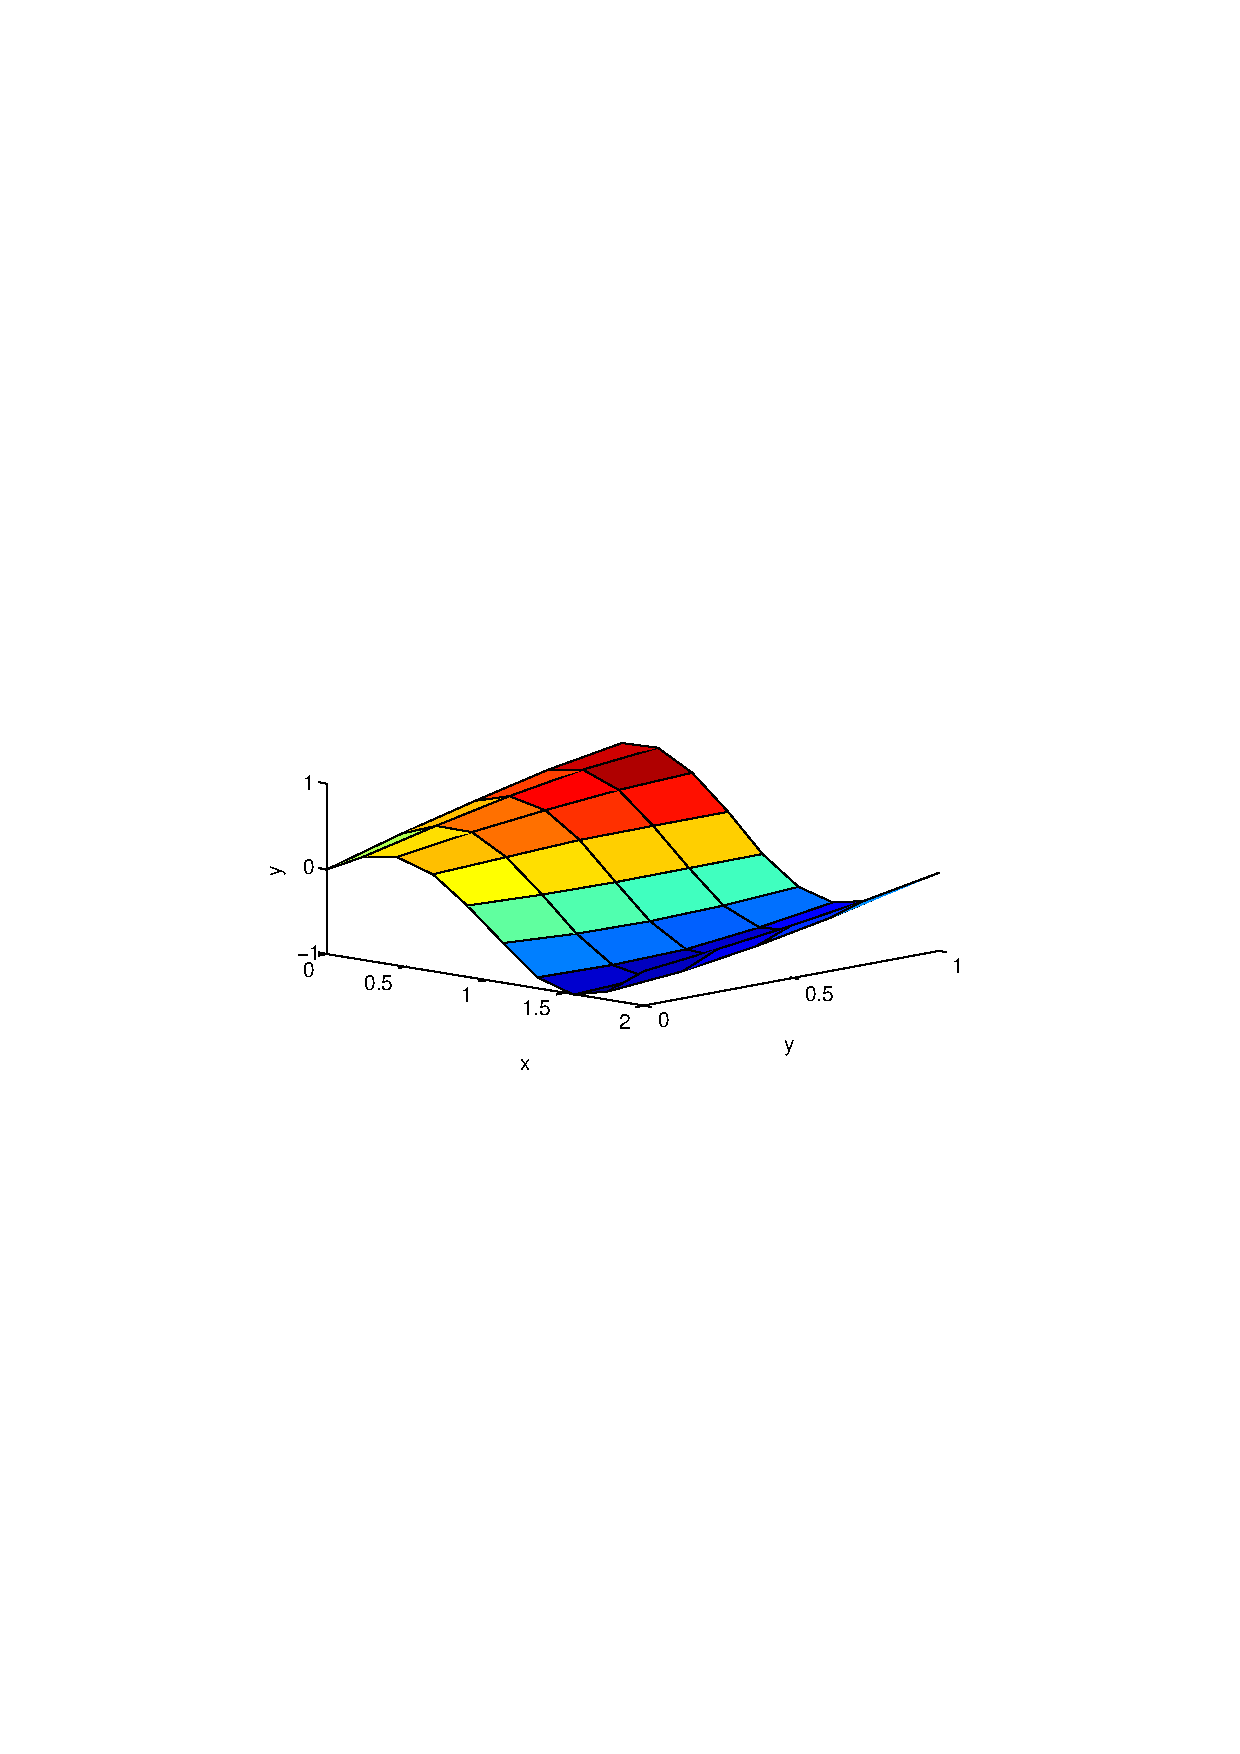
\includegraphics[width=0.45\linewidth, trim=3cm 11cm 3cm 11cm]{figure/X.pdf}
% 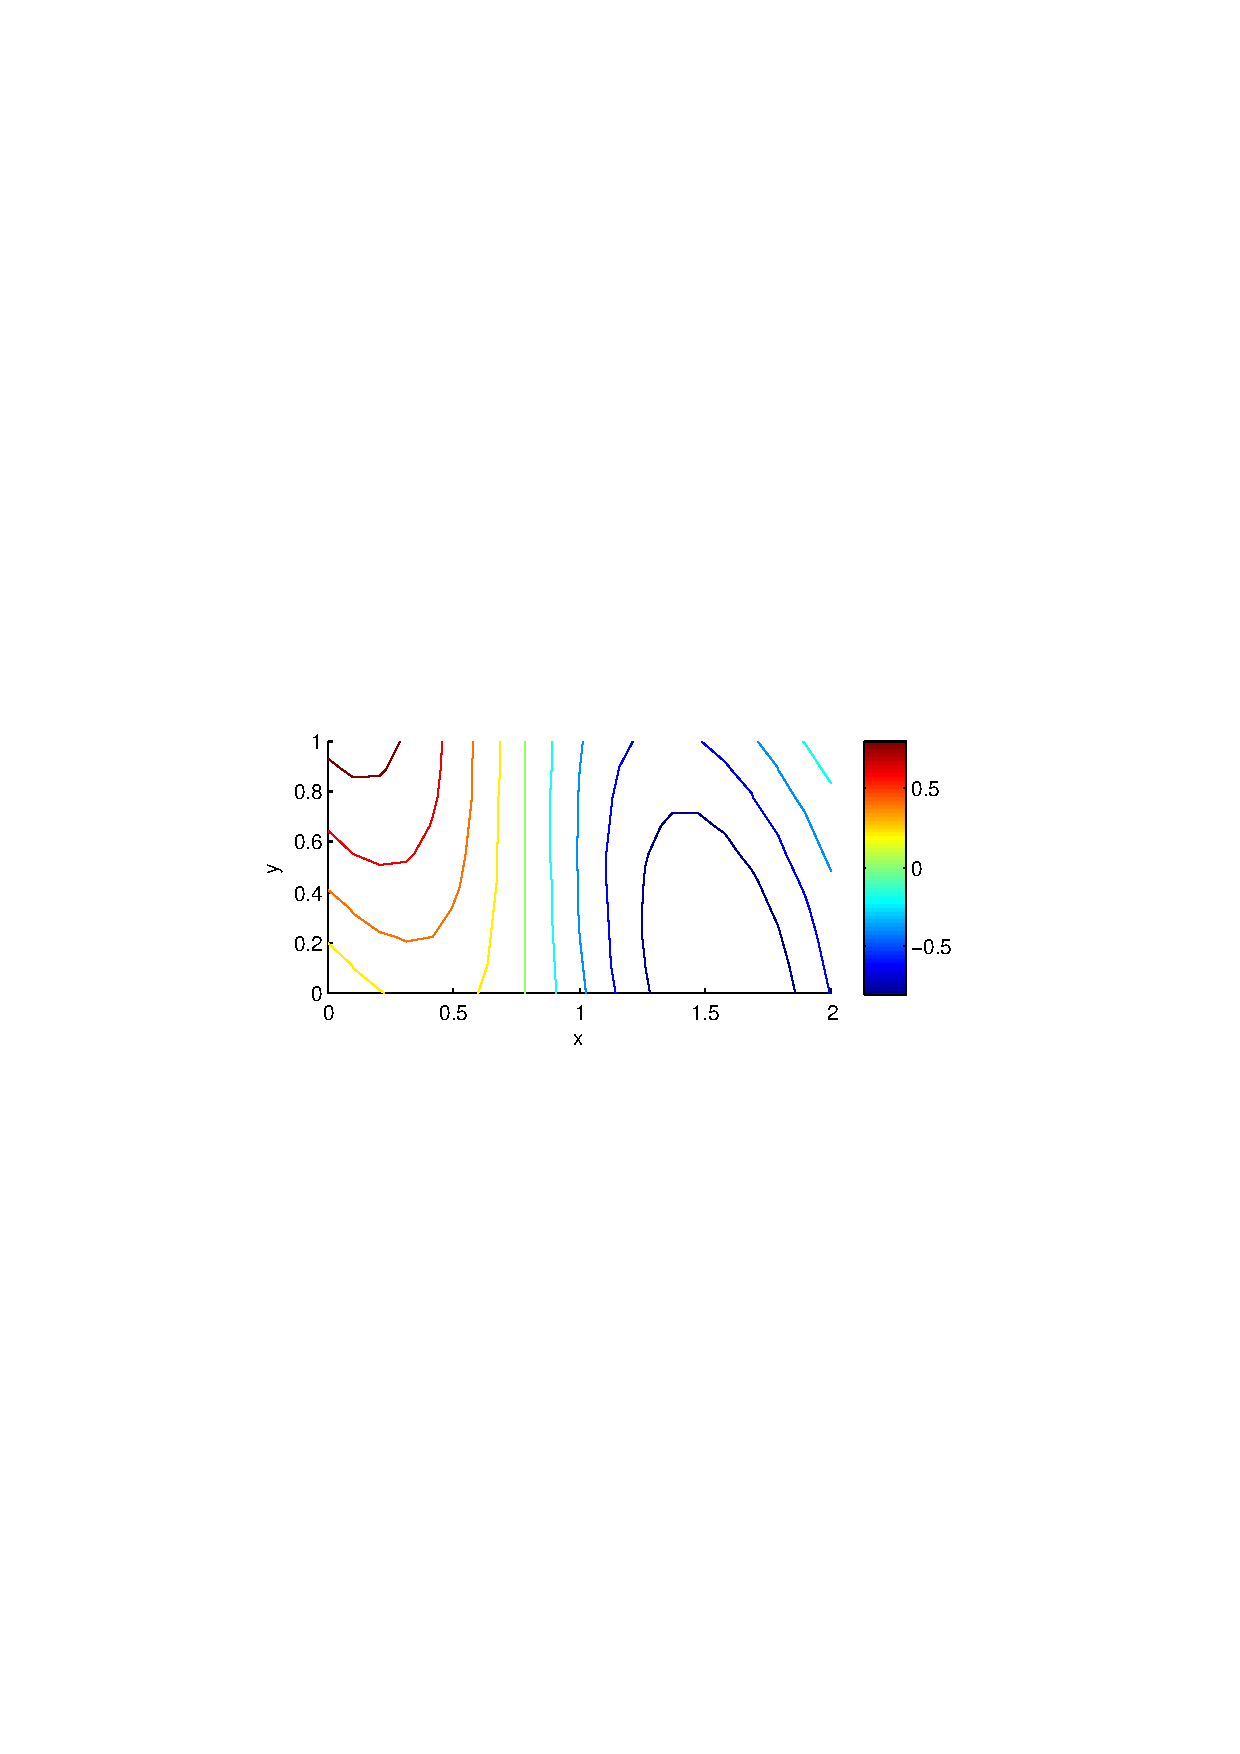
\includegraphics[width=0.45\linewidth, trim=3cm 11cm 3cm 11cm]{figure/Y.pdf}
% \caption{Surface and contour plots showing the two dimensional function $z(x,y)=\sin(x+y)\cos(2x)$.} % Figure text below figure
% \end{figure}
% 
% \section{Equation}
% \begin{equation}
% f(t)=\left\{ \begin{array}{ll}
% 1,~~~~ & t< 1 \\
% t^2 & t\geq 1
% \end{array}\right.
% \end{equation}
% 
% \section{Table}
% \begin{table}[H]
% \centering
% \caption{Values of $f(t)$ for $t=0,1,\dots 5$.}
% \begin{tabular}{l|llllll} \hline\hline
% $t$ & 0 & 1 & 2 & 3 & 4 & 5 \\ \hline
% $f(t)$ & 1 & 1 & 4 & 9 & 16 & 25 \\ \hline\hline
% \end{tabular}
% \end{table}
% 
% \section{Chemical structure}
% \begin{center}
% \chemfig{X*5(-E-T-A-L-)}
% \end{center}
% 
% 
% \section{Source code listing}
% \begin{minted}[frame=single]{matlab}
% % Generate x- and y-nodes
% x=linspace(0,1); y=linspace(0,1);
% 
% % Calculate z=f(x,y)
% for i=1:length(x)
%  for j=1:length(y)
%   z(i,j)=x(i)+2*y(j);
%  end
% end
% \end{minted}
% 
% \subsection{Other alternatives to the Theory chapter}
% Sometimes, it is more appropriate to name this chapter Background.
% 
% At CSE, there exists a large span of different types of thesis works. Sometimes it is more appropriate to join the Theory and Methods chapters, sometimes the Theory chapter would be so small that it should be a subsection. Talk to your supervisor to find the most appropriate structure for your thesis.


% CREATED BY DAVID FRISK, 2016
\chapter{Theory: Lenses}\label{chapter:lenses}
This chapter covers the first theoretical part of the work, consisting mainly of formal proofs of different categorical properties of the category \textbf{Poly}. All code is available open source at GitHub \cite{code}, which is recommended to follow while reading the thesis.

\section{The category \textbf{Poly}}

The category \textbf{Poly} is the category of polynomial endofunctors in \textbf{Set}, with morphisms as natural transformations. They are called \textit{Polynomial} because these functors can be written down as high-school algebraic expressions, like:
$$p(y) = y^2 +4y + 10$$
But instead of handling numbers, these polynomial expressions have \textit{sets} plugged into the variable \textit{y}.
Sum, multiplication, exponentiation, and numeric literals, are all considered in the context of sets. A numeric literal such as $7$ represents the set $\underline{7}$, a set with 7 elements. A $+$ symbol corresponds to \textit{the categorical coproduct}, multiplication  corresponds to \textit{the categorical product} and exponentiation to the exponential object: in this context, it is the type of functions from the exponent to the base of the term. For example, $ f : 7^2 \cong f : 2 \rightarrow 7$. This way of thinking algebraically is very convenient, because plugging in "numbers" into the polynomial expressions to get "numbers" back will turn out to be a very useful kind of operation.

\subsection{Objects are polynomial functors}

The objects of \textbf{Poly} are polynomial functors, which can be written as expressions like the one shown above. Since \textbf{Poly} handles sets, though, more unorthodox looking expressions can be created. For instance, the polynomial below is perfectly coherent:
\begin{equation}
p(y) = \mathbb{N}y^2 + 1
\label{eqn.natpoly}
\end{equation}
and it can be thought of as taking a set as input, and sending it to the set of: either infinitely long tuples of functions from $\underline{2}$ to this set, or to the only element of the singleton set. Like the poly-book, each summand of a power of $y$ in the polynomials are referred to as a \textit{position}, and the exponent of that power as a \textit{direction at that position}
\footnote{Note: The book acknowledges the unfortunate naming clash with the equivalent category of containers, where in that context, positions are called directions and directions are called shapes.}.
This suggests that a polynomial has a set of positions, and for each element in this set, a set of directions. Therefore, a natural way to represent these polynomials in Agda is as a dependent set:

\begin{minted}{agda}
record Polynomial : Set₁ where
    constructor mkpoly
    field
        position : Set
        direction : position → Set
\end{minted}
The way to write the example $p(y) = \mathbb{N}y^2 + 1$ in Agda using this type is then
\mint{agda}{p = mkpoly (ℕ ⊎ ⊤)  λ {(inj₁ x) → Bool ; (inj₂ y) → ⊥}}

Sometimes, a polynomial is referred to as having "a single position" when it is a \textit{monomial}.
This means that, in the definition of such a polynomial, the set of directions does not depend on the set of positions.
For instance, the monomial
$$
p(y) = \mathbb{R}y^{\{a, b, c, d\}}
$$
does not have any dependence between \textit{the set of positions} (the real numbers) and \textit{the sets of directions} (the set $\{a, b, c, d\}$).
The sets of directions would normally be a family of sets, where each position could give a different one, but in this case, they're always the same set.
This way of phrasing positions might be unsettling at first, but it makes more sense in everyday programming with polynomial functors, since what really matters when handling dependent sets is what distinction an indexing set performs. 
If two positions index the same set, they can be thought as the same thing.

\subsection*{More perspectives on polynomials}

Understanding polynomial functors is crucial, and there are many ways to think about them.
The book showcases other standard ways to visualize polynomials, which are helpful to interpret the category in different applications and to build intuition about the purely categorical perspective. One of these is \textit{corolla forests}:

\begin{equation}
  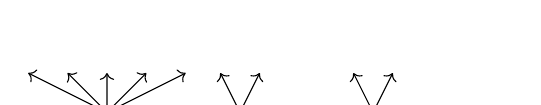
\begin{tikzpicture}[trees]
    \node (1) {$\bullet$} 
      child {}
      child {}
      child {}
      child {}
      child {};
    \node[right=1.5 of 1] (2) {$\bullet$} 
      child {}
      child {};
    \node[right=1.5 of 2] (3) {$\bullet$} 
      child {}
      child {};
    \node[right=1.5 of 3] (4) {$\bullet$};
  \end{tikzpicture}
\label{eqn:corollafirstexample}
\end{equation}

The term \textit{corolla} refers to a tree with a depth of one, and \textit{forest} refers to the fact that there are many such small trees.
The set of positions is the set of roots of the forest (in this case $\underline{4}$), and the set of directions at each position is the set of arrows at each root (in this case $\underline{5}$, $\underline{2}$, $\underline{2}$ and $\underline{0}$).
This then corresponds to $p(y) = y^5 + y^2 + y^2 + 1 \cong y^5 + 2y^3 + 1$. This perspective lends intuition to the decision-making interpretation of polynomials. Very loosely speaking, the set of directions is "directions in which one can go" given that one is at that set's associated position. Since polynomials can handle infinite sets, even uncountably infinite ones, one can imagine such infinite corolla trees. For example, the polynomial \ref{eqn.natpoly} could be visualized as:

\begin{align}

\begin{tikzpicture}[trees]
  \node (1) {$\bullet$}
    ;
  \node[right=0.5 of 1] (2) {$\bullet$} 
    child {}
    child {};
  \node[right=0.5 of 2] (3) {$\bullet$} 
    child {}
    child {};
  \node[right=0.5 of 3] (4) {$\bullet$} 
    child {}
    child {};
  \node[right=.5 of 4] (5) {$\cdots$};
\end{tikzpicture}
\end{align}

Another perspective on polynomials, emphasizing the container datatype view, is as Haskell algebraic data types.
The polynomial \ref{eqn:corollafirstexample}, for instance, can be written in Haskell as:
\begin{minted}{haskell}
data P y = Fst y y y y y | Snd y y | Trd y y | Frth
  deriving Functor
\end{minted}
This type can trivially implement the \texttt{Functor} typeclass, so much so that it can be derived automatically as above (given that the language extension \texttt{DeriveFunctor} is enabled).

% KEEP COMMENTED: Infinite set in directions
% \[%\label{eqn.represented_interval}
% \begin{tikzpicture}[trees, sibling distance=0.0625mm]
%   \node (1) {$\bullet$} 
%     child[sibling distance=3mm] foreach \i in {1,2,3}
%     ;
%   \node[right=1 of 1] (2) {$\bullet$} 
%     child foreach \i in {1,...,160}
%     ;
%   \node[right=1 of 2] (3) {$\bullet$} 
%     child foreach \i in {1,...,160}
%     ;
%   \node[right=1 of 3] (4) {$\bullet$} 
%     child foreach \i in {1,...,160}
%     ;
%   \node[right=.7 of 4] (5) {$\cdots$};
% \end{tikzpicture}
% \]

As functors, polynomials act on both objects and functions, and this is defined as:
\begin{minted}{agda}
_⦅_⦆ : Polynomial → Set → Set
_⦅_⦆ (mkpoly position direction) Y = Σ position λ x → (direction x → Y)
infixl 30 _⦅_⦆

applyFn : {A B : Set} → (p : Polynomial) → (A → B) → p ⦅ A ⦆ → p ⦅ B ⦆
applyFn (mkpoly position direction) f (fst , snd) = fst , λ x → f (snd x)
\end{minted}

Then, these definitions can be used to prove that \textbf{Poly}'s objects really are functors. 
A record in \texttt{agda-categories} is formulated corresponding to an endofunctor in the library's provided instance of \textbf{Set}:

\begin{minted}{agda}
F-resp : {p : Polynomial} {A B : Set} {f g : A → B} {x : p ⦅ A ⦆ } → 
    f ≡ g → applyFn p f x ≡ applyFn p g x
F-resp {x = posApp , dirApp} pr = λ i → posApp , (pr i) ∘  dirApp

conv : {A B : Set} {f g : A → B} → ({x : A} → f x Eq.≡ g x) → f ≡ g
conv p = funExt λ _ → eqToPath p

asEndo : (p : Polynomial) → Functor (Sets zero) (Sets zero)
asEndo p = record
    { F₀ = λ x → p ⦅ x ⦆
    ; F₁ = λ f → applyFn p f
    ; identity = Eq.refl
    ; homomorphism = Eq.refl
    ; F-resp-≈ = λ {_} {_} {f} {g} proof → 
        pathToEq (F-resp {f = f} {g = g} (conv proof))
    }
\end{minted}


\subsection{Arrows are natural transformations - \textit{dependent lenses}}

Arrows on \textbf{Poly} are so-called \textit{dependent lenses}.
The reason is that arrows between monomials are the usual definition of lenses in Haskell, as a pair of non-dependent "getter and setter" functions. For example, a lens between $Sy^T$ and $Ay^B$ consists of the functions \mintinline{agda}{get : S → A} and \mintinline{agda}{set : S → B → T}. 
A dependent lens has the additional property that "the types we are allowed to set depend on the value we get".
This notion is explored further in the applications part of the thesis. 
Since non-dependent lenses (lenses between monomials) are a very special case of dependent lenses, the arrows in \textbf{Poly} are referred to as simply \textit{lenses}.

\subsection*{Perspectives on lenses}
Another use of the corolla forest perspective is that it makes visualizing maps between polynomials intuitive.
Consider the polynomials $p(y) = y^5 + 2y^2 + y$ and $q(y) = y^3 + y^2 + 2y + 1$.
First, their visualization as corollas is as:


\[
\begin{tikzpicture}[rounded corners]
	\node (p1) [draw, green!50!black, "$p$" above] {
	\begin{tikzpicture}[trees, sibling distance=2.5mm]
    \node["\tiny 1" below] (1) {$\bullet$} 
      child {}
      child {}
      child {}
      child {}
      child {};
    \node[right=1.0 of 1,"\tiny 2" below] (2) {$\bullet$} 
      child {}
      child {};
    \node[right=1.0 of 2,"\tiny 3" below] (3) {$\bullet$}
      child {}
      child {};
    \node[right=1.0 of 3,"\tiny 4" below] (4) {$\bullet$}
      child {};
  \end{tikzpicture}
  };
%
	\node (p2) [draw, red!75!black, right=2 of p1, "$q$" above] {
	
\begin{tikzpicture}[trees, sibling distance=2.5mm]
    \node["\tiny A" below] (1) {$\bullet$} 
      child {}
      child {}
      child {};
    \node[right=1.0 of 1,"\tiny B" below] (2) {$\bullet$} 
      child {}
      child {};
    \node[right=1.0 of 2,"\tiny C" below] (3) {$\bullet$}
      child {};
    \node[right=1.0 of 3,"\tiny D" below] (4) {$\bullet$}
      child {};
    \node[right=1.0 of 4,"\tiny E" below] (5) {$\bullet$}
    ;
  \end{tikzpicture}
  };
\end{tikzpicture}
\]
A map between $p$ and $q$ can be visualized in the following way.
Each position in $p$ is sent to a position in $q$, and for each of these sendings, its directions are sent back to the directions at the original position:
\[
\begin{tikzpicture}
	\node (p1) {
	\begin{tikzpicture}[trees, sibling distance=2.5mm]
    \node[green!50!black, "{\color{green!50!black}\tiny 1}" below] (1) {$\bullet$} 
      child[green!50!black] {coordinate (11)}
      child[green!50!black] {coordinate (12)}
      child[green!50!black] {coordinate (13)}
      child[green!50!black] {coordinate (14)}
      child[green!50!black] {coordinate (15)};
    \node[right=1.5 of 1, red!75!black, "{\color{red!75!black}\tiny A}" below] (2) {$\bullet$} 
      child[red!75!black] {coordinate (21)}
      child[red!75!black] {coordinate (22)}
      child[red!75!black] {coordinate (23)};
    \draw[|->, shorten <= 3pt, shorten >= 3pt] (1) -- (2);
    \begin{scope}[densely dotted, bend right, decoration={markings, mark=at position 0.75 with \arrow{stealth}}]
      \draw[postaction={decorate}] (21) to (11);
      \draw[postaction={decorate}] (22) to (12);
      \draw[postaction={decorate}] (23) to (13);
    \end{scope}
  \end{tikzpicture}	
	};	
%
	\node (p2) [right=1 of p1] {
	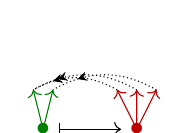
\begin{tikzpicture}[trees, sibling distance=2.5mm]
    \node[green!50!black, "{\color{green!50!black}\tiny 2}" below] (1) {$\bullet$} 
    child[green!50!black] {coordinate (11)}
    child[green!50!black] {coordinate (12)};
    \node[right=of 1, red!75!black, "{\color{red!75!black}\tiny A}" below] (2) {$\bullet$} 
      child[red!75!black] {coordinate (21)}
      child[red!75!black] {coordinate (22)}
      child[red!75!black] {coordinate (23)};
    \draw[|->, shorten <= 3pt, shorten >= 3pt] (1) -- (2);
    \begin{scope}[densely dotted, bend right, decoration={markings, mark=at position 0.75 with \arrow{stealth}}]
      \draw[postaction={decorate}] (21) to (11);
      \draw[postaction={decorate}] (22) to (11);
      \draw[postaction={decorate}] (23) to (12);
    \end{scope}
  \end{tikzpicture}	
	};	
%
	\node (p3) [right=1 of p2] {
	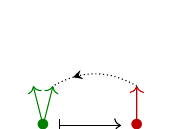
\begin{tikzpicture}[trees, sibling distance=2.5mm]
    \node[green!50!black, "{\color{green!50!black}\tiny 3}" below] (1) {$\bullet$} 
      child[green!50!black] {coordinate (11)}
      child[green!50!black] {coordinate (12)};
    \node[right=of 1, red!75!black, "{\color{red!75!black}\tiny C}" below] (2) {$\bullet$} 
      child[red!75!black] {coordinate (21)};
		;
    \draw[|->, shorten <= 3pt, shorten >= 3pt] (1) -- (2);
    \begin{scope}[densely dotted, bend right, decoration={markings, mark=at position 0.75 with \arrow{stealth}}]
      \draw[postaction={decorate}] (21) to (12);

    \end{scope}
  \end{tikzpicture}	
	};	
 	\node (p4) [below right=-1.05cm and 1 of p3] {
	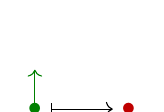
\begin{tikzpicture}[trees, sibling distance=2.5mm]
    \node[green!50!black, "{\color{green!50!black}\tiny 4}" below] (1) {$\bullet$} 
    child[green!50!black];
    \node[right=of 1, red!75!black, "{\color{red!75!black}\tiny E}" below] (2) {$\bullet$} 
		;
    \draw[|->, shorten <= 3pt, shorten >= 3pt] (1) -- (2);
  \end{tikzpicture}	
	};	
\end{tikzpicture}
\]

If instead the map on the directions also goes forward, it would be another kind of arrow called charts. Charts are the arrows in the category \textbf{Chart}, which is the second category this thesis explores, in chapter \ref{chapter:charts}.

In the Haskell view of polynomials, lenses can be given as the following type synonym (requires \texttt{RankNTypes} language extension):
\begin{minted}{haskell}
type Lens p q = forall y. p y -> q y
\end{minted}

An example of a lens between the two polynomials above would look like the following (requires \texttt{LambdaCase} language extension):
\newpage
\begin{minted}{haskell}
data P y = Fst y y y y y | Snd y y | Trd y y | Frth
  deriving Functor

data Q y = A y y y | B y y | C y | D y | E
  deriving Functor

exampleLens :: Lens P Q
exampleLens = \case
  Fst y1 y2 y3 y4 y5 -> _
  Snd y1 y2 -> _
  Trd y1 y2 -> _
  Frth -> _
\end{minted}

The map on positions translates to a map on value constructors; for each of the summands of $p$, first a value constructor in $q$ must be chosen. After choosing a constructor, its values must be filled in:

\begin{minted}{haskell}
exampleLens :: Lens P Q
exampleLens = \case
  Fst y1 y2 y3 y4 y5 -> A y1 y2 y3
  Snd y1 y2 -> A y1 y1 y2
  Trd y1 y2 -> C y2
  Frth -> E
\end{minted}

This recovers the idea of a function "back", that is a map on directions \textit{at that position}: for each of the targeted value constructors in $q$, a lens must fill its slots with the source constructor's $y$ values. 
For example, in this case, the three slots of the \texttt{A} constructor in the first branch must be filled by the five available choices in the source constructor \texttt{Fst}.
In an abstract sense, we can see this as a function of type $\underline{3} \rightarrow \underline{5}$ - a choice of source out of 5 possible sources for each of the 3 slots.

Expressing more general kinds of lenses in Haskell using this scheme becomes hard quickly however.
The dependency between the value of the map on positions and the type of the map of directions is hidden and baked into the syntax of the language. 
There are attempts to do this in Haskell \cite{iceland_jack_thread} \cite{sjoerd_gist}, but the Haskell view is given only for the sake of perspective. Polynomials and lenses are much more natural in Agda.

\subsection*{Lenses in Agda}
Here is their definition:

\begin{minted}{agda}
record Lens (from to : Polynomial) : Set where
    constructor _⇆_
    open Polynomial
    field
        mapPosition : position from → position to
        mapDirection : (fromPos : position from) → 
                       direction to (mapPosition fromPos) → 
                       direction from fromPos
\end{minted}

The constructor \mintinline{agda}{_⇆_} is an attempt at representing the two maps: on positions below and going forward (because they are the coefficients of the polynomials) and on directions on top going backwards (because they are exponents of $y$ at each position).

As they are maps between functors, one can expect that lenses are natural transformations. Indeed, they are, and here is how to formulate them as such in the context of \texttt{agda-categories}:

\begin{minted}{agda}
asNatTransLens : {p q : Polynomial} → 
            Lens p q → 
            NaturalTransformation (asEndo p) (asEndo q)
asNatTransLens (f ⇆ f♯) = record { 
    η = λ { X (posP , dirP) → f posP , dirP ∘ f♯ posP } ; 
    commute = λ f₁ → Eq.refl ; 
    sym-commute = λ f₁ → Eq.refl 
    }
\end{minted}

Two more pieces of data are needed to form a valid category: the identity arrow and composition. 

\subsubsection{The identity lens}
The identity lens leaves the polynomial untouched in both the positions and the direction at each position, which is implemented by the identity function.

\begin{minted}{agda}
idLens : {A : Polynomial} → Lens A A
idLens = id ⇆ λ _ → id
\end{minted}

\subsubsection{Composing lenses}
Composition of lenses is done in the natural way. The composed maps on positions are obtained with straightforward function composition. The same is true of the maps on directions, but with some extra work to deal with the fact that they are dependent functions.

\begin{minted}{agda}
_∘ₚ_ : {A B C : Polynomial} → Lens B C → Lens A B → Lens A C
_∘ₚ_ (f ⇆ f♯) (g ⇆ g♯) = (f ∘ g) ⇆ (λ i → g♯ i ∘ f♯ (g i))
\end{minted}

\subsection{Categorical axioms}

That the associativity and identity laws hold for \textbf{Poly} follows directly from the definitions of these types, which means that they can be proved via Cubical Agda's \mintinline{agda}{refl}.
With all the pieces in place, the full formulation of \textbf{Poly} as a category in \texttt{agda-categories}' is provided:

\begin{minted}{agda}
-- Categorical/Poly/Instance.agda
∘-resp-≈ : {A B C : Polynomial} 
           {f h : Lens B C} 
           {g i : Lens A B} → 
           f ≡ h → g ≡ i → (f ∘ₚ g) ≡ (h ∘ₚ i)
∘-resp-≈  p q ii = (p ii) ∘ₚ (q ii)

Poly : Category (lsuc lzero) lzero lzero
Poly = record
    { Obj = Polynomial
    ; _⇒_ = Lens
    ; _≈_ = _≡_
    ; id = idLens
    ; _∘_ = _∘ₚ_
    ; assoc = refl
    ; sym-assoc = refl
    ; identityˡ = refl
    ; identityʳ = refl
    ; identity² = refl
    ; equiv = record { refl = refl ; sym = sym ; trans = _∙_ }
    ; ∘-resp-≈ = ∘-resp-≈
    }
\end{minted}

This record definition should not be surprising: \textbf{Poly}'s objects are \mintinline{agda}{Polynomial}s, its arrows are dependent \mintinline{agda}{Lens}es, the notion of equality between arrows is defined to be cubical equality \mintinline{agda}{_≡_}, the identity lens and composition are the previously defined values in Agda.
The rest of the data provided to the record correspond to the categorical laws plus some convenience that \texttt{agda-categories} provides: for instance, the proof \mintinline{agda}{sym-assoc} is not normally needed, but it makes it so that the opposite of opposite categories are equal "on the nose" to the original categories, and not just provably equal. 
A more detailed overview of the design decisions of \texttt{agda-categories} can be found in \cite{agda-cats}.

\section{Polynomial equality}
There are some occasions where polynomials need to be compared for equality.
For example, to prove the right unit law for the parallel product (explained later) $\otimes$ with Y as unit: \mintinline{agda}{rightUnit : (p q : Polynomial) → p ⊗ Y ≡ p}.
% aw a convenient way of characterizing monoidal structures in \textbf{Poly} is by simply expressing the laws on types,
%  which requires polynomials to be compared; for instance, the right unit 
%(in the case of monoidal structures, we stick to the \texttt{agda-categories} framework and don't rely on equality of objects at all, but polynomial equality is both useful elsewhere and an illuminating exercise).

Since a polynomial is a record consisting of the \mintinline{agda}{position : Set} and \newline \mintinline{agda}{direction : position → Set} a characterization of equality for this record is needed to make it easy to use and prove equalities between polynomials.
An alternative definition of a polynomial as a Σ-type is used in aid to characterize the equality, to use the many properties and lemmas about Σ-type in the Cubical library.
That Σ-type, along with proofs that the definitions are the same are:

\begin{minted}{agda}
PolyAsSigma : Set₁
PolyAsSigma = Σ[ position ∈ Set ] (position → Set)

polyToSigma : Polynomial → PolyAsSigma
polyToSigma (mkpoly position direction) = position , direction
    
polyFromSigma : PolyAsSigma → Polynomial
polyFromSigma (position , direction) = mkpoly position direction

poly≡polySigma : Polynomial ≡ PolyAsSigma
poly≡polySigma = isoToPath (iso polyToSigma 
                                polyFromSigma 
                                (λ _ → refl) 
                                (λ _ → refl))
\end{minted}

Equality for the Σ-type is then implemented by using \mintinline{agda}{ΣPathTransport→PathΣ} from the Cubical library.
It is important to note that an equality of a Σ-type is a Σ of equalities.
This means that a proof that the map on positions is equals is needed, as well as a proof that the map on directions is equal.
Subst is needed for the proof on the directions to make the types match.

\begin{minted}{agda}
polySigmas≡ : (a b : PolyAsSigma)
    → (fstA≡fstB : fst a ≡ fst b)
    → (subst (λ x → x → Type) fstA≡fstB (snd a)) ≡ snd b
    → a ≡ b
polySigmas≡ a b fstA≡fstB sndA≡sndB
  = ΣPathTransport→PathΣ a b (fstA≡fstB , sndA≡sndB)
\end{minted}

This definition of equality is then transferred to the record definition of Polynomials leading to the final characterization of polynomials equality:
\begin{minted}{agda}
poly≡ : {a b : Polynomial}
    → (fstA≡fstB : position a ≡ position b)
    → (subst (λ x → x → Type) fstA≡fstB (direction a)) ≡ direction b
    → a ≡ b
poly≡ {a} {b} fstA≡fstB sndA≡sndB i
  = polyFromSigma (polySigmas≡ (polyToSigma a)
                               (polyToSigma b) 
                               fstA≡fstB 
                               sndA≡sndB 
                               i)
\end{minted}

In addition, an all quantified version of equality is used which simplifies some proofs:
\begin{minted}{agda}
poly≡∀ : {a b : Polynomial}
    → (fstA≡fstB : position a ≡ position b)
    → ((posB : position b) → 
       subst (λ x → x → Type) fstA≡fstB (direction a) posB ≡ direction b posB)
    → a ≡ b
poly≡∀ {a} {b} fstA≡fstB sndA≡sndB
  = poly≡ fstA≡fstB λ i x → sndA≡sndB x i
\end{minted}

\section{Lens equality}
In category theory, it is frequently of interest to know when two morphisms are equal. Therefore, also a characterization of equality for lenses are needed. 
This characterization of equality needs to be convenient enough to be usable in practical proofs.

A lens consists of two components, with the second component depending on the first. 
This suggests a Σ-type structure, which leads to a strategy similar to polynomial equality, but in lenses things are more complicated, since the underlying types are functions instead of simple sets.
Still, representing lenses as Σ-types is straightforward:

\begin{minted}{agda}
LensAsSigma : Polynomial → Polynomial → Type
LensAsSigma (mkpoly posP dirP) (mkpoly posQ dirQ)
    = Σ[ mapPos ∈ (posP → posQ) ]
    ((fromPos : posP) → dirQ (mapPos fromPos) → dirP fromPos)
    
sigmaToLens : LensAsSigma p q → Lens p q
sigmaToLens (mapPos , mapDir) = mapPos ⇆ mapDir

lensToSigma : Lens p q → LensAsSigma p q
lensToSigma  (mapPos ⇆ mapDir) = mapPos , mapDir

lens≡lensSigma : (Lens p q) ≡ (LensAsSigma p q)
lens≡lensSigma = isoToPath (iso lensToSigma
                                sigmaToLens 
                                (λ _ → refl)
                                (λ _ → refl))
\end{minted}

Equality for this $\Sigma$-type is defined and then transferred to the lens type:

\begin{minted}{agda}
lensSigmas≡ : {p q : Polynomial} (f g : LensAsSigma p q)
    → (fstF≡fstG : fst f ≡ fst g)
    → subst (λ mapPos → (fromPos : position p) → 
            direction q (mapPos fromPos) → 
            direction p fromPos) 
            fstF≡fstG
      (snd f) ≡ snd g
    → f ≡ g
lensSigmas≡ f g fstF≡fstG sndF≡sndG 
  = ΣPathTransport→PathΣ f g (fstF≡fstG , sndF≡sndG)

lens≡ : {p q : Polynomial} {f g : Lens p q}
    → (mapPos≡ : mapPosition f ≡ mapPosition g) 
    → subst (λ mapPos → (fromPos : position p) → 
                        direction q (mapPos fromPos) → 
                        direction p fromPos) mapPos≡ 
      (mapDirection f) ≡ mapDirection g
    → f ≡ g
lens≡ {p} {q} {f} {g} mapPos≡ mapDir≡ i
  = sigmaToLens ((lensSigmas≡ {q = q} (lensToSigma f) 
                                      (lensToSigma g) 
                                      mapPos≡ 
                                      mapDir≡ 
                                      i))
\end{minted}

An all quantified version of lens equality is provided as well, named \mintinline{agda}{lens≡∀∀}:

Both \mintinline{agda}{lens≡} and \mintinline{agda}{lens≡∀∀} provide a way to prove equalities between lenses.
However, in some cases they are limited and almost impossible to use.
The reason is that subst is not very deep in the term, and the subst is of a complicated dependent function type, where the dependent function returns a new function with the domain varying.
Often, it is possible to use subst laws to push subst further into the term, which would make the type easier to use.
This idea is captured by the more powerful variant of lens equality, \mintinline{agda}{lens≡ₚ}.
For \mintinline{agda}{lens≡ₚ}, subst is pushed further into the term making it much more practical to use in proofs.

\begin{minted}{agda}
lens≡ₚ : {p q : Polynomial} {f g : Lens p q}
  → (mapPosEq : mapPosition f ≡ mapPosition g)
  → (
          (x : position p) → 
          (y : direction q (mapPosition g x)) → 
          mapDirection f x  
          (subst (λ mapPos → direction q (mapPos x)) (sym mapPosEq) y) 
          ≡ 
          mapDirection g x y
      )
  → f ≡ g
lens≡ₚ {f = f} {g = g} a b i
  = sigmaToLens (lensSigmas≡ₚ {f = f} {g = g} a b i)
\end{minted}

To implement \mintinline{agda}{lens≡ₚ}, or more specifically, \mintinline{agda}{lensSigmas≡ₚ}, \mintinline{agda}{ΣPathP} is used instead of \mintinline{agda}{ΣPathTransport→PathΣ}.

\begin{minted}{agda}
lensSigmas≡ₚ : {p q : Polynomial} {f g : Lens p q}
  → (mapPosEq : Lens.mapPosition f ≡ Lens.mapPosition g)
  → ((x : position p) → (y : direction q (mapPosition g x)) → mapDirection f x  (subst (λ mapPos → direction q (mapPos x)) (sym mapPosEq) y) ≡ mapDirection g x y)
  → lensToSigma f ≡ lensToSigma g
lensSigmas≡ₚ {p = p} {q = q} {f = f} {g = g} mapPosEq mapDirEq
    = ΣPathP (mapPosEq , 
        funExt λ x →
        funExtDep λ {y1} {y2} p →
          cong (mapDirection f x) (fromPathP⁻ p) ∙ mapDirEq x y2)
\end{minted}

\subsection*{If lenses and polynomials are both Σ-types in disguise, why not just use Σ-types?}

The main reason is \textit{usability}. This is a convenience-driven decision: we want our implementation of \textbf{Poly} to not only be amenable to formalization and having theorems proven about it, but also to be \textit{nice to program in}. Working with Σ-types causes readability to suffer too much, because the names of the constructor and fields are lost. We then make the compromise of converting between the record Σ-type representations only in the equality modules, since the proofs that the representations are equal allows us to carry equality over between the types, a very useful feature of Cubical Agda.



\section{Initial object}
An object is called initial if there exists an unique arrow from it to every other object in the category. In \textbf{Poly}, the initial object is the polynomial $p(y) = 0$ with no positions (and therefore also no directions). It is the functor that sends any set to the empty set.

\begin{minted}[escapeinside=||]{agda}
|$\mathbb{0}$| : Polynomial
|$\mathbb{0}$| = mkpoly ⊥ λ ()
\end{minted}

The steps to prove that $\mathbb{0}$ is the initial object is to firstly construct a lens to every other object, and to secondly show that this lens is unique. 

Since $\mathbb{0}$ has no positions (nor directions) both the map on positions and the map on directions to any other polynomial $p$ is given by the function \mintinline{agda}{λ ()} (often named absurd) from the empty type.
\begin{minted}[escapeinside=||]{agda}
lensFromZero : {p : Polynomial} → Lens |$\mathbb{0}$| p
lensFromZero = (λ ()) ⇆ (λ ())
\end{minted}

The final step is to show that this lensFromZero from $\mathbb{0}$ to $p$ is unique. This is done by assuming that there exists another lens $f$ from $\mathbb{0}$ to $p$ and then prove that $f$ actually is the same lens as lensFromZero. 

\begin{minted}[escapeinside=||]{agda}
lensFromZeroUnique : {p : Polynomial} (f : Lens |$\mathbb{0}$| p) → lensFromZero ≡ f
lensFromZeroUnique _ = lens≡ (funExt λ ()) (funExt λ ())
\end{minted}

This is implemented by using the lens equality function and the fact that the absurd function (from the empty type) is unique utilizing function extensionality. We plug these proofs into the \texttt{agda-categories} characterization of the initial object:

\begin{minted}[escapeinside=||]{agda}
open import Categories.Object.Initial Poly

zeroIsInitial : IsInitial |$\mathbb{0}$|
zeroIsInitial = record { ! = lensFromZero ; !-unique = lensFromZeroUnique }

initialZero : Initial
initialZero = record { ⊥ = |$\mathbb{0}$| ; ⊥-is-initial = zeroIsInitial }
\end{minted}



\section{Terminal object}
Dually to the initial object, the terminal object is an object such that there is a unique arrow from every other object in the category to it. In \textbf{Poly}, the terminal object is defined as the polynomial with a single position, but no directions for that position. It is the functor that sends all sets to the singleton set.

\begin{minted}[escapeinside=||]{agda}
|$\mathbb{1}$| : Polynomial
|$\mathbb{1}$| = mkpoly ⊤ (λ _ → ⊥)
\end{minted}

Similarly to the initial object, to show that $\mathbb{1}$ is a terminal object is to first construct a lens \textbf{from} every other object, and to show that each of these lenses is unique.

The map on positions from any other polynomial to $\mathbb{1}$ is the function always returning unit (often also named unit). For this position, the map on directions goes from $\bot$ since $\mathbb{1}$ has no directions, thus the map on directions is again the absurd function.

\begin{minted}[escapeinside=||]{agda}
lensToOne : {p : Polynomial} → Lens p |$\mathbb{1}$|
lensToOne = (λ _ → tt) ⇆ λ _ ()
\end{minted}

Finally, for uniqueness, any other lens $f$ from $p$ to $\mathbb{1}$ is the same as lensToOne. For map on positions equality, refl is used to show that any two functions (with same domain) to $\top$ is the same. For map on directions equality, uniqueness of the absurd function is used, as in the initial object. The more advanced version of lens equality is used to do the function extensionality in the background, allowing for more concise syntax.

\begin{minted}[escapeinside=||]{agda}
lensToOneUnique : {p : Polynomial} (f : Lens p |$\mathbb{1}$|) →  lensToOne ≡ f
lensToOneUnique _ = lens≡∀∀ refl (λ _ ())
\end{minted}

And again we plug these proofs in to the \texttt{agda-categories} characterization of the initial object:

\begin{minted}[escapeinside=||]{agda}
open import Categories.Object.Terminal Poly

oneIsTerminal : IsTerminal
oneIsTerminal = record { ! = lensToOne ; !-unique = lensToOneUnique }

terminalOne : Terminal
terminalOne = record { ⊤ = |$\mathbb{1}$| ; ⊤-is-terminal = oneIsTerminal }
\end{minted}

\section{Product}
% https://q.uiver.app/?q=WzAsNCxbMCwzLCJBIl0sWzQsMywiQiJdLFsyLDIsIkEgXFx0aW1lcyBCIl0sWzIsMCwiVCJdLFsyLDAsIlxccGlfMSIsMV0sWzIsMSwiXFxwaV8yIiwxXSxbMywyLCIhIiwxLHsic3R5bGUiOnsiYm9keSI6eyJuYW1lIjoiZGFzaGVkIn19fV0sWzMsMCwiaCIsMV0sWzMsMSwiayIsMV1d
\begin{figure}
  \[\begin{tikzcd}
    && T \\
    \\
    && {A \times B} \\
    A &&&& B
    \arrow["{\pi_1}"{description}, from=3-3, to=4-1]
    \arrow["{\pi_2}"{description}, from=3-3, to=4-5]
    \arrow["{!}"{description}, dashed, from=1-3, to=3-3]
    \arrow["h"{description}, from=1-3, to=4-1]
    \arrow["k"{description}, from=1-3, to=4-5]
  \end{tikzcd}\]
  \caption{Product diagram of two objects $A$ and $B$.}
  \label{fig:productDiagram}
\end{figure}

The product of two objects $A$ and $B$ is an object $A \times B$ together with arrows $\pi_1$ and $\pi_2$ such that, given any other object $T$ and arrows from $T$ to $A$ and $B$, the diagram in Figure \ref{fig:productDiagram} commutes and the arrow $!$ exists and is unique. The arbitrary object $T$ can be intuitively thought of as a "candidate" object to be the product. This is an example of a \textit{universal property} in category theory and the arrows $h$ and $k$ are said to be \textit{factorized} through the compositions $\pi_1 \circ  !$ and $\pi_2 \circ !$ respectively.

\textbf{Poly} has all products, which means that for any two polynomials $p$ and $q$ we can construct their product as the polynomial $p*q$.

Firstly, the product polynomial of two polynomials is defined. The position set is the product of $p$'s and $q$'s position sets, while the direction at a position is either a direction of $p$ or a direction of $q$. This is another instance of the fact that these polynomials behave just like the ones in high school algebra: for example, given $p(y) = y^2$ and $q(y) = 5y^3 + 2y$, their product is given by $p * q (y) = 5y^5 + 2y^3$. In Agda, the product is given as:

\begin{minted}{agda}
_*_ : Polynomial → Polynomial → Polynomial
(mkpoly posP dirP) * (mkpoly posQ dirQ) =
    mkpoly (posP × posQ) (λ {(posP , posQ) → (dirP posP) ⊎ (dirQ posQ)})
\end{minted}

A visualization of the product is provided in Figure \ref{fig:productExample}.
\begin{figure}[H]
  \[
    \begin{tikzpicture}[rounded corners]
      \node (prod) [draw, "$p * q$" above] {
      \begin{tikzpicture}[trees, sibling distance=2.5mm, rounded corners]
        \node["\tiny {\color{green!50!black} {1},\color{red!75!black} {A}}" below] (1a) {$\bullet$}
          % First row
          child [green!50!black] {}
          child [green!50!black] {}
          child [green!50!black] {}
          child [green!50!black] {}
          child [green!50!black] {}
          child [red!75!black] {}
          child [red!75!black] {}
          child [red!75!black] {};
        \node["\tiny {\color{green!50!black} {1},\color{red!75!black} {B}}" below, right=1.5 of 1a] (1b) {$\bullet$} 
          child [green!50!black] {}
          child [green!50!black] {}
          child [green!50!black] {}
          child [green!50!black] {}
          child [green!50!black] {}
          child [red!75!black] {}
          child [red!75!black] {};
        \node["\tiny {\color{green!50!black} {1},\color{red!75!black} {C}}" below, right=1.5 of 1b] (1c) {$\bullet$} 
          child [green!50!black] {}
          child [green!50!black] {}
          child [green!50!black] {}
          child [green!50!black] {}
          child [green!50!black] {}
          child [red!75!black] {};
        \node["\tiny {\color{green!50!black} {1},\color{red!75!black} {D}}" below, right=1.5 of 1c] (1d) {$\bullet$} 
          child [green!50!black] {}
          child [green!50!black] {}
          child [green!50!black] {}
          child [green!50!black] {}
          child [green!50!black] {}
          child [red!75!black] {};
        \node["\tiny {\color{green!50!black} {1},\color{red!75!black} {D}}" below, right=1.5 of 1d] (1e) {$\bullet$} 
          child [green!50!black] {}
          child [green!50!black] {}
          child [green!50!black] {}
          child [green!50!black] {}
          child [green!50!black] {};
        % Second row
        \node["\tiny {\color{green!50!black} {2},\color{red!75!black} {A}}" below, below=1.0 of 1a] (2a) {$\bullet$} 
          child [green!50!black] {}
          child [green!50!black] {}
          child [red!75!black] {}
          child [red!75!black] {}
          child [red!75!black] {};
        \node["\tiny {\color{green!50!black} {2},\color{red!75!black} {B}}" below, below=1.0 of 1b] (2b) {$\bullet$} 
          child [green!50!black] {}
          child [green!50!black] {}
          child [red!75!black] {}
          child [red!75!black] {};
        \node["\tiny {\color{green!50!black} {2},\color{red!75!black} {C}}" below, below=1.0 of 1c] (2c) {$\bullet$} 
          child [green!50!black] {}
          child [green!50!black] {}
          child [red!75!black] {};
        \node["\tiny {\color{green!50!black} {2},\color{red!75!black} {D}}" below, below=1.0 of 1d] (2d) {$\bullet$} 
          child [green!50!black] {}
          child [green!50!black] {}
          child [red!75!black] {};
        \node["\tiny {\color{green!50!black} {2},\color{red!75!black} {E}}" below, below=1.0 of 1e] (2e) {$\bullet$} 
          child [green!50!black] {}
          child [green!50!black] {};
        % Third row
        \node["\tiny {\color{green!50!black} {3},\color{red!75!black} {A}}" below, below=1.0 of 2a] (3a) {$\bullet$} 
          child [green!50!black] {}
          child [green!50!black] {}
          child [red!75!black] {}
          child [red!75!black] {}
          child [red!75!black] {};
        \node["\tiny {\color{green!50!black} {3},\color{red!75!black} {B}}" below, below=1.0 of 2b] (3b) {$\bullet$} 
          child [green!50!black] {}
          child [green!50!black] {}
          child [red!75!black] {}
          child [red!75!black] {};
        \node["\tiny {\color{green!50!black} {3},\color{red!75!black} {C}}" below, below=1.0 of 2c] (3c) {$\bullet$} 
          child [green!50!black] {}
          child [green!50!black] {}
          child [red!75!black] {};
        \node["\tiny {\color{green!50!black} {3},\color{red!75!black} {D}}" below, below=1.0 of 2d] (3d) {$\bullet$} 
          child [green!50!black] {}
          child [green!50!black] {}
          child [red!75!black] {};
        \node["\tiny {\color{green!50!black} {3},\color{red!75!black} {E}}" below, below=1.0 of 2e] (3e) {$\bullet$} 
          child [green!50!black] {}
          child [green!50!black] {};
        % Fourth row
        \node["\tiny {\color{green!50!black} {4},\color{red!75!black} {A}}" below, below=1.0 of 3a] (4a) {$\bullet$} 
          child [green!50!black] {}
          child [red!75!black] {}
          child [red!75!black] {}
          child [red!75!black] {};
        \node["\tiny {\color{green!50!black} {4},\color{red!75!black} {B}}" below, below=1.0 of 3b] (4b) {$\bullet$} 
          child [green!50!black] {}
          child [red!75!black] {}
          child [red!75!black] {};
        \node["\tiny {\color{green!50!black} {4},\color{red!75!black} {C}}" below, below=1.0 of 3c] (4c) {$\bullet$} 
          child [green!50!black] {}
          child [red!75!black] {};
        \node["\tiny {\color{green!50!black} {4},\color{red!75!black} {D}}" below, below=1.0 of 3d] (4d) {$\bullet$} 
          child [green!50!black] {}
          child [red!75!black] {};
        \node["\tiny {\color{green!50!black} {4},\color{red!75!black} {E}}" below, below=1.0 of 3e] (4e) {$\bullet$} 
          child [green!50!black] {};
        
      \end{tikzpicture}
      };
      \node (p1) [draw, green!50!black, left=1.0 of prod, "$p$" above] {
      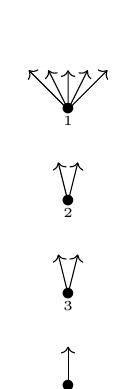
\begin{tikzpicture}[trees, sibling distance=2.5mm]
        \node["\tiny 1" below] (1) {$\bullet$} 
          child {}
          child {}
          child {}
          child {}
          child {};
        \node[below=1.0 of 1,"\tiny 2" below] (2) {$\bullet$} 
          child {}
          child {};
        \node[below=1.0 of 2,"\tiny 3" below] (3) {$\bullet$}
          child {}
          child {};
        \node[below=1.0 of 3,"\tiny 4" below] (4) {$\bullet$}
          child {};
      \end{tikzpicture}
      };
    %
      \node (p2) [draw, red!75!black, below=1 of prod, "$q$" above] {
      \begin{tikzpicture}[trees, sibling distance=2.5mm]
        \node["\tiny A" below] (1) {$\bullet$} 
          child {}
          child {}
          child {};
        \node[right=1.5 of 1,"\tiny B" below] (2) {$\bullet$} 
          child {}
          child {};
        \node[right=1.5 of 2,"\tiny C" below] (3) {$\bullet$}
          child {};
        \node[right=1.5 of 3,"\tiny D" below] (4) {$\bullet$}
          child {};
        \node[right=1.5 of 4,"\tiny E" below] (5) {$\bullet$}
        ;
      \end{tikzpicture}
      };
    \end{tikzpicture}
    \]
    
    \caption{$p(y) = y^5 + 2y^2 + y$, $q(y) = y^3 + y^2 + 2y + 1$. Their product $p * q$ has both $p$ and $q$'s positions; each position of $p * q$ is a pair with one position of $p$ and one of $q$. The direction at that position of $p * q$ is the disjoint union of the directions at the originals, with the arrow's color indicating where they came from.}
    \label{fig:productExample}
\end{figure}

Continuing with Figure \ref{fig:productDiagram}, $\pi_1$ and $\pi_2$ are defined to take the projections on the positions, and injections on the map on the directions back. In Figure \ref{fig:productExample}, this can be imagined by selecting only the correspondingly colored part of a corolla in the product corolla forest. 

\begin{minted}{agda}
π₁ : {p q : Polynomial} → Lens (p * q) p
π₁ = proj₁ ⇆ λ _ → inj₁

π₂ : {p q : Polynomial} → Lens (p * q) q
π₂ = proj₂ ⇆ λ _ → inj₂
\end{minted}

Given an object $c$ as the domain of two lenses $f$ and $g$, $\langle f,g \rangle$ should be the factorization lens of $f$ and $g$. This factorization must be unique, which is proved later as the last step. The factorization lens is defined by taking the pair of functions for map on positions. For the map on directions either f or g is used depending on the direction.

\begin{minted}{agda}
⟨_,_⟩ : {p q r : Polynomial} → Lens p q → Lens p r → Lens p (q * r)
⟨ f ⇆ f♯ , g ⇆ g♯ ⟩ = < f , g > ⇆ λ posP → [ f♯ posP , g♯ posP ]
\end{minted}

Finally, we need to supply the proofs associated with the product. There are two proofs needed to show that the diagram \ref{fig:productDiagram} commutes, and one for showing the uniqueness of $\langle f,g \rangle$. The proofs for commuting is shown with \texttt{refl}, but the uniqueness is left out for space reasons - this will be done relatively frequently in the rest of the thesis, since many of these proofs get quite long. Interested readers can of course see the code for the formalization \cite{code}. But the idea is that if we have another factorization lens $h$ it must be the same as $\langle f,g \rangle$. 

\begin{minted}{agda}
project₁ : {p q r : Polynomial} {f : Lens r p} {g : Lens r q} →
           π₁ ∘ₚ ⟨ f , g ⟩ ≡ f
project₁ = refl

project₂ : {p q r : Polynomial} {f : Lens r p} {g : Lens r q} →
           π₂ ∘ₚ ⟨ f , g ⟩ ≡ g
project₂ = refl

unique : {p q r : Polynomial} {h : Lens p (q * r)} {f : Lens p q} 
    {g : Lens p r → (π₁ ∘ₚ h) ≡ f} →
    (π₂ ∘ₚ h) ≡ g → 
    ⟨ f , g ⟩ ≡ h
unique = ...
    where
        lemma : ⟨ π₁ ∘ₚ h , π₂ ∘ₚ h ⟩ ≡ h
        lemma = ...
\end{minted}

\subsection{Productized lens}
Two lenses between different pairs of polynomials can be represented as a single lens between two products, as follows.

\begin{minted}{agda}
⟨_×_⟩ : {a b c d : Polynomial} → (f : Lens a c) (g : Lens b d)
    → Lens (a * b) (c * d)
⟨ (f ⇆ f♯) × (g ⇆ g♯) ⟩ 
    = (λ {(a , b) → f a , g b}) ⇆
        λ {(a , b) (inj₁ dirC) → inj₁ (f♯ a dirC)
         ; (a , b) (inj₂ dirD) → inj₂ (g♯ b dirD)}
\end{minted}

\subsection{Generalized product}
Similarly to how the $\Pi$ type is a generalization of the product type in \textbf{Type}, we can create the product of all polynomials indexed by any type. Think of it as a "fold", in the sense that each element of a set produces a new polynomial that is productized with the "accumulator" of this fold (all the products taken so far). This construction will be particularly important for the exponential object.

\begin{minted}{agda}
ΠPoly : Σ[ indexType ∈ Set ] (indexType → Polynomial) → Polynomial
ΠPoly (indexType , generatePoly) = mkpoly pos dir
  where
    -- Embedding all polynomial positions into one position
    pos : Set
    pos = (index : indexType) → position (generatePoly index)

    -- Direction is exactly one of the polynomials' directions
    dir : pos → Set
    dir pos = Σ[ index ∈ indexType ] direction (generatePoly index) (pos index) 
\end{minted}

Using this generalized product type with \texttt{Bool} as the index type is equivalent to having a normal binary product - which makes sense, since it means taking a product of two polynomials. This is proved in \texttt{Various.agda}.

\begin{minted}{agda}
productIsΠPoly : {p q : Polynomial}
    → ΠPoly (Bool , tupleToFunFromBool (p , q)) ≡ (p * q) 
productIsΠPoly = ...

tupleToFunFromBool : {ℓ : Level} {A : Set ℓ} → (A × A) → Bool → A
tupleToFunFromBool (a , b) true = a
tupleToFunFromBool (a , b) false = b
\end{minted}

With the generalized product it is also useful to have the factorizer $\langle f,g \rangle$ generalized, now factorizing a generalized amount of lenses instead of just $f$ and $g$.

% -- An arrow A→(B*C) is the same as two functions A→B and A→C
\begin{minted}{agda}
universalPropertyProduct : {p : Polynomial} {Index : Type} 
    {generate : Index → Polynomial}
    → Lens p (ΠPoly (Index , generate)) ≡ ((i : Index) → Lens p (generate i))
universalPropertyProduct = ...
\end{minted}

\subsection{Monoid}

The product forms a monoid with $\mathbb{1}$, which we show by constructing a monoidal category (\textbf{Poly}, $\times$, $\mathbb{1}$). In fact, the product is a \textit{symmetric} monoidal structure, since $A \times B$ is isomorphic to $B \times A$. This is one place where the existing structure of \texttt{agda-categories} is extremely useful, as we only need to call some of its helpers to prove this and rely on the fact that all cartesian categories form monoidal categories with respect to the product. The code for it is:

\begin{minted}{agda}
-- Categorical/Poly/Monoidal/Product.agda

open import Categories.Category.Monoidal
import Categories.Category.Cartesian as Cartesian

binaryProducts : Cartesian.BinaryProducts Poly
binaryProducts = record { product = prod }

cartesian : Cartesian.Cartesian Poly
cartesian = record { terminal = terminalOne ; 
                     products = binaryProducts }

productMonoidal : Monoidal Poly
productMonoidal 
    = Cartesian.CartesianMonoidal.monoidal Poly cartesian

open import Categories.Category.Monoidal.Symmetric productMonoidal
productSymmetricMonoidal : Symmetric
productSymmetricMonoidal 
    = Cartesian.CartesianSymmetricMonoidal.symmetric Poly cartesian
\end{minted}

\newpage

\section{Coproduct}
The coproduct is the dual construction to the product, obtained from reversing all arrows, shown in figure \ref{fig:coproductDiagram}.

\begin{figure}[H]
  % https://q.uiver.app/?q=WzAsNCxbMCwzLCJBIl0sWzQsMywiQiJdLFsyLDIsIkEgKyBCIl0sWzIsMCwiVCJdLFswLDIsIlxcdGV4dHtpbmp9XzEiLDFdLFsxLDIsIlxcdGV4dHtpbmp9XzIiLDFdLFsyLDMsIiEiLDEseyJzdHlsZSI6eyJib2R5Ijp7Im5hbWUiOiJkYXNoZWQifX19XSxbMCwzLCJoIiwxXSxbMSwzLCJrIiwxXV0=
  \[\begin{tikzcd}
    && T \\
    \\
    && {A + B} \\
    A &&&& B
    \arrow["{\text{i}_1}"{description}, from=4-1, to=3-3]
    \arrow["{\text{i}_2}"{description}, from=4-5, to=3-3]
    \arrow["{!}"{description}, dashed, from=3-3, to=1-3]
    \arrow["h"{description}, from=4-1, to=1-3]
    \arrow["k"{description}, from=4-5, to=1-3]
  \end{tikzcd}\]
  \caption{Coproduct diagram of $A$ and $B$.}
  \label{fig:coproductDiagram}
  \end{figure}

\textbf{Poly} has all coproducts, given any $p$ and $q$, the coproduct $p+q$ is defined by taking the (Set) coproduct on the positions and the \textit{projection} on the directions. Again, consider the analogy with high-school algebra. Given two polynomials $p(y) = 4y^2$ and $q(y) = y^2 + 3y$, their sum is given by $(p + q)(y) \cong 4y^2 + y^2 + 3y \cong 5y^2 + 3y$. In this example, four of the positions with $2$ as a direction came from $p$ and one of them came from $q$, hence in the Agda code for it below, we pattern match on the resulting polynomials's position. As a shorthand, we use Agda's \mintinline{agda}{[_,_]} function.

\begin{minted}{agda}
_+_ : Polynomial → Polynomial → Polynomial
(mkpoly posA dirA) + (mkpoly posB dirB) = mkpoly (posA ⊎ posB) [ dirA , dirB ]
\end{minted}

A visualization of an example coproduct is provided in figure \ref{fig:coproductExample}.

\begin{figure}[H]
\[
\begin{tikzpicture}[rounded corners]
	\node (p1) [draw, green!50!black, "$p$" above] {
	\begin{tikzpicture}[trees, sibling distance=2.5mm]
    \node["\tiny 1" below] (1) {$\bullet$} 
      child {}
      child {}
      child {}
      child {}
      child {};
    \node[right=1.0 of 1,"\tiny 2" below] (2) {$\bullet$} 
      child {}
      child {};
    \node[right=1.0 of 2,"\tiny 3" below] (3) {$\bullet$};
  \end{tikzpicture}
  };
%
	\node (p2) [draw, red!75!black, right=2 of p1, "$q$" above] {
	
\begin{tikzpicture}[trees, sibling distance=2.5mm]
    \node["\tiny A" below] (1) {$\bullet$} 
      child {}
      child {}
      child {};
    \node[right=1.0 of 1,"\tiny B" below] (2) {$\bullet$}
      child {};
    \node[right=1.0 of 2,"\tiny C" below] (3) {$\bullet$}
      child {};
    \node[right=1.0 of 3,"\tiny D" below] (4) {$\bullet$}
    ;
  \end{tikzpicture}
  };
\end{tikzpicture}
\]
\[
  \begin{tikzpicture}[rounded corners]
    \node (sum) [draw, right=2 of p1, "$p + q$" above] {
    \begin{tikzpicture}[trees, sibling distance=2.5mm]
      \node[green!50!black, "\tiny {\color{green!50!black}1}" below] (1) {$\bullet$} 
        child [green!50!black] {}
        child [green!50!black] {}
        child [green!50!black] {}
        child [green!50!black] {}
        child [green!50!black] {};
      \node[red!75!black, right=1.0 of 1,"\tiny {\color{red!75!black}A}" below] (a) {$\bullet$} 
        child [red!75!black] {}
        child [red!75!black] {}
        child [red!75!black] {};
      \node[green!50!black, right=1.0 of a,"\tiny {\color{green!50!black}2}" below] (2) {$\bullet$}
        child [green!50!black] {}
        child [green!50!black] {};
      \node[red!75!black, right=1.0 of 2,"\tiny {\color{red!75!black}B}" below] (b) {$\bullet$}
        child [red!75!black] {};
      \node[red!75!black, right=1.0 of b,"\tiny {\color{red!75!black}C}" below] (c) {$\bullet$}
        child [red!75!black] {};
      \node[green!50!black, right=1.0 of c,"\tiny {\color{green!50!black}3}" below] (3) {$\bullet$}
      ;
      \node[red!75!black, right=1.0 of 3,"\tiny {\color{red!75!black}D}" below] (d) {$\bullet$}
      ;
    \end{tikzpicture}
    };
  \end{tikzpicture}
\]
\caption{A sum of polynomials $p(y) = y^5 + y^2 + 1$ and $q(y) = y^3 + 2y + 1$. The resulting polynomial has the disjoint union of both as its positions, and each position has the directions at that position in the original polynomial it came from.}
\label{fig:coproductExample}
\end{figure}


The injections $i_1$ and $i_2$ are defined by taking the injections on the positions and keeping the directions on that position using $id$. The example \ref{fig:coproductDiagram} shows how $i_1$ behave for one position. 

\begin{minted}{agda}
i₁ : {p q : Polynomial} → Lens p (p + q)
i₁ = inj₁ ⇆ λ _ → id

i₂ : {p q : Polynomial} → Lens q (p + q)
i₂ = inj₂ ⇆ λ _ → id
\end{minted}


Given an object $c$ as the codomain of two functions $f$ and $g$, $[f,g]$ should be the (unique) factorization lens of f and g. This function is defined by using $f$ or $g$'s behavior depending what the position corresponds to.


\begin{minted}{agda}
[_,_]ₚ : {p q r : Polynomial} → Lens p r → Lens q r → Lens (p + q) r
[ f ⇆ f♯ , g ⇆ g♯ ]ₚ = [ f , g ] ⇆ [ f♯ , g♯ ]
\end{minted}

The proofs needed correspond to the ones from the product. 
\begin{minted}{agda}
inject₁ : {f : Lens p a} {g : Lens q a} → [ f , g ]ₚ ∘ₚ i₁ ≡ f
inject₁ = refl

inject₂ : {f : Lens p a} {g : Lens q a} → [ f , g ]ₚ ∘ₚ i₂ ≡ g
inject₂ = refl

unique : {F : Polynomial} {h : Lens (A + B) F} {f₁ : Lens A F} {f₂ : Lens B F} 
    → (h ∘ₚ i₁) ≡ f₁
    → (h ∘ₚ i₂) ≡ f₂
    → [ f₁ , f₂ ]ₚ ≡ h
unique p₁ p₂ = ...
    where
        lemma : [ h ∘ₚ i₁ , h ∘ₚ i₂ ]ₚ ≡ h
        lemma = ...
        
\end{minted}


\subsection{Generalized coproduct}
The coproduct can also be generalized to work with any amount of polynomials indexed by an index-type. This corresponds to the sigma type, or exists operator.
\begin{minted}{agda}
ΣPoly : Σ[ indexType ∈ Set ] (indexType → Polynomial) → Polynomial
ΣPoly (indexType , generatePoly) = mkpoly pos dir
  where
    -- It is the positions of one of the polynomials
    pos : Set 
    pos = Σ[ index ∈ indexType ] (position (generatePoly index))

    -- It is the direction of the polynomial for the position
    dir : pos → Set
    dir (index , positionAtIndex) = direction (generatePoly index)
                                              positionAtIndex
\end{minted}

Using the generalized coproduct with bool as index type, we recover the normal binary coproduct. This is proved in \texttt{Various.agda}.

\begin{minted}{agda}
coproductIsΣPoly : {p q : Polynomial}
  → ΣPoly (Bool , tupleToFunFromBool (p , q)) ≡ p + q
coproductIsΣPoly = ...
\end{minted}

The generalized factorizer for the generalized coproduct can now be defined.

\begin{minted}{agda}
-- A function (A+B)→C is the same as two functions A→C and B→C
universalPropertyCoproduct : {Index : Type} {generate : Index → Polynomial}
   → Lens (ΣPoly (Index , generate)) p ≡ ((i : Index) → Lens (generate i) p)
universalPropertyCoproduct = ...
\end{minted}

\subsection{Monoid}
To show the coproduct is a monoid, we do almost the same as for the product. Again we rely on \texttt{agda-categories}' helpers to define the monoidal category (\textbf{Poly}, $+$, $\mathbb{0}$) - which is also \textit{symmetric} monoidal. This time we rely on the fact that the category is \textit{co-}cartesian, but the code is almost identical:
\begin{minted}{agda}
-- Categorical/Poly/Monoidal/Coproduct.agda

open import Categories.Category.Monoidal
import Categories.Category.Cocartesian as Cocartesian

binaryCoproducts : Cocartesian.BinaryCoproducts Poly
binaryCoproducts = record { coproduct = coprod }

coproductCocartesian  : Cocartesian.Cocartesian Poly
coproductCocartesian = record { initial = initialZero ;
                                coproducts = binaryCoproducts }

coproductMonoidal : Monoidal Poly
coproductMonoidal = 
  Cocartesian.CocartesianMonoidal.+-monoidal Poly coproductCocartesian

open import Categories.Category.Monoidal.Symmetric coproductMonoidal
productSymmetricMonoidal : Symmetric
productSymmetricMonoidal = 
  Cocartesian.CocartesianSymmetricMonoidal.+-symmetric Poly coproductCocartesian
\end{minted}

\subsection{Coproductized lens}
It is also easy to define a parallel coproduct lens. Like for the product, two lenses can be made to represent a single lens between coproducts.
\begin{minted}{agda}
⟨_⊎_⟩ : {p q r w : Polynomial} → (f : Lens p r) (g : Lens q w)
         → Lens (p + q) (r + w)
⟨_⊎_⟩ {p} {q} {r} {w} (f ⇆ f♯) (g ⇆ g♯) = mp ⇆ md
    where mp : position (p + q) → position (r + w)
          mp = map f g
          md : (fromPos : position (p + q)) → 
               direction (r + w) (mp fromPos) → 
               direction (p + q) fromPos
          md (inj₁ x) d = f♯ x d
          md (inj₂ y) d = g♯ y d
infixl 30 ⟨_⊎_⟩
\end{minted}

\section{Parallel product} \label{section:parallelProduct}
The parallel product (also called Dirichlet product) is another useful binary operator on polynomials. It is defined as the pair of positions and pair of directions. This is the first operator that does not have a direct high school algebra correspondence, as it multiplies on both coefficients and exponents: given $p(y) = 2y^4 + 3y^2$ and $q(y) = 2y^3$, $(p \otimes q)(y) = 4y^{12} + 6y^6$.

\begin{minted}{agda}
_⊗_ : Polynomial → Polynomial → Polynomial
(mkpoly posA dirA) ⊗ (mkpoly posB dirB)
    = mkpoly (posA × posB) (λ (posA , posB) → (dirA posA) × (dirB posB))
\end{minted}

The parallel product will turn out to be extremely important in the context of dynamical systems. More on this in the applications chapter. A visualization of it is provided in Figure \ref{fig:parallelProductExample}.

\begin{figure}[H]
  \[
    \begin{tikzpicture}[rounded corners]
      \node (prod) [draw, "$p \otimes q$" above] {
      \begin{tikzpicture}[trees, sibling distance=2.5mm, rounded corners]
        \node["\tiny {\color{green!50!black} {1},\color{red!75!black} {A}}" below] (1a) {$\bullet$} 
          % First row
          child {}
          child {}
          child {}
          child {}
          child {}
          child {};
        \node["\tiny {\color{green!50!black} {1},\color{red!75!black} {B}}" below, right=1.5 of 1a] (1b) {$\bullet$} 
          child {}
          child {}
          child {};
        \node["\tiny {\color{green!50!black} {1},\color{red!75!black} {C}}" below, right=1.5 of 1b] (1c) {$\bullet$};
        \node[above=0.5 of 1a] {\tiny {{\color{green!50!black}x},{\color{red!75!black}a} {\color{green!50!black}x},{\color{red!75!black}b} {\color{green!50!black}y},{\color{red!75!black}a} ... {\color{green!50!black}z},{\color{red!75!black}b}}};
        \node[above=0.5 of 1b] {\tiny {{\color{green!50!black}x},{\color{red!75!black}c} {\color{green!50!black}y},{\color{red!75!black}c} {\color{green!50!black}z},{\color{red!75!black}c}}};

        % Second row
        \node["\tiny {\color{green!50!black} {2},\color{red!75!black} {A}}" below, below=1.0 of 1a] (2a) {$\bullet$} 
          child {}
          child {};
        \node["\tiny {\color{green!50!black} {2},\color{red!75!black} {B}}" below, below=1.0 of 1b] (2b) {$\bullet$} 
          child {};
        \node["\tiny {\color{green!50!black} {2},\color{red!75!black} {C}}" below, below=1.0 of 1c] (2c) {$\bullet$};
        \node[above=0.5 of 2a] {\tiny {{\color{green!50!black}w},{\color{red!75!black}a} {\color{green!50!black}w},{\color{red!75!black}b}}};
        \node[above=0.5 of 2b] {\tiny {{\color{green!50!black}w},{\color{red!75!black}c}}};
      \end{tikzpicture}
      };
      \node (p1) [draw, green!50!black, left=1.0 of prod, "$p$" above] {
      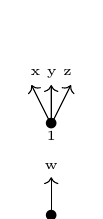
\begin{tikzpicture}[trees, sibling distance=2.5mm]
        \node["\tiny 1" below] (1) {$\bullet$} 
        child {}
        child {}
        child {};
        \node[below=1.0 of 1,"\tiny 2" below] (2) {$\bullet$} 
          child {};
        \node[above=0.5 of 1] {\tiny {x y z}};
        \node[above=0.5 of 2] {\tiny w};
        \end{tikzpicture}
      };
    %
      \node (p2) [draw, red!75!black, below=1 of prod, "$q$" above] {
      \begin{tikzpicture}[trees, sibling distance=2.5mm]
        \node["\tiny A" below] (1) {$\bullet$} 
          child {}
          child {};
        \node[right=1.5 of 1,"\tiny B" below] (2) {$\bullet$} 
          child {};
        \node[right=1.5 of 2,"\tiny C" below] (3) {$\bullet$}
        ;
        \node[above=0.5 of 1] {\tiny {a b}};
        \node[above=0.5 of 2] {\tiny c};
      \end{tikzpicture}
      };
    \end{tikzpicture}
    \]
    
    \caption{$p(y) = y^3 + y$, $q(y) = y^2 + y + 1$. Like the regular product, their parallel product $p \otimes q$ has both $p$ and $q$'s positions, with each  position of $p \otimes q$ being a pair with one position of $p$ and one of $q$. However, the directions at that position of $p \otimes q$ is the product of the directions at the originals, with each direction being a pair of the original directions.}
    \label{fig:parallelProductExample}
\end{figure}


\subsection{Monoid}

The parallel product forms a monoid with $y$. Since it is not the canonical product (or coproduct), as far as we know, we can't rely on the previous tricks to construct a monoidal category out of it. However, we can define the monoidal category construction manually, which is a lot of code in "volume", so we omit it from the text. The code can be found in \texttt{Categorical/Poly/Monoidal/ParallelProduct.agda}.

\subsection{Parallel lens}

The parallel product also enables turning to lenses, between individual polynomials, into one that goes between the parallel products. Here is the definition in Agda:

\begin{minted}{agda}
⟨_⊗_⟩ : {p q r w : Polynomial} → Lens p r → Lens q w → 
      Lens (p ⊗ q) (r ⊗ w)
⟨_⊗_⟩ {p} {q} {r} {w} (f ⇆ f♯) (g ⇆ g♯) = mp ⇆ md
  where mp : position (p ⊗ q) → position (r ⊗ w)
        mp (posp , posq) = f posp , g posq
        md : (fromPos : position (p ⊗ q)) → 
             direction (r ⊗ w) (mp fromPos) → 
             direction (p ⊗ q) fromPos
        md (posp , posq) (dirr , dirw) = f♯ posp dirr , g♯ posq dirw
\end{minted}

This particular action will have deep implications in the applications chapter.

\section{Composition product}
\label{section:composition}
Since polynomials are functors, and in fact \textit{endo}functors, they can be composed to give rise to new polynomial functors. The composition operator is given by the symbol ◂. Here we can recover high-school algebra intuition. Composing functors corresponds to plugging in entire expressions, instead of numbers, into a polynomial. For instance, given $p(y) = y^2$ and $q(y) = y^2 + 3y$, the composition product is given as $(p \triangleleft q)(y) = (y^2 + 3y)^2$.

\begin{minted}{agda}
-- Proposition 5.2, page 158. Note: not same definition used. 
-- We here treat positions  as inhabitants of the same set, 
-- which makes a lot of proofs easier down the line.
_◂_ : Polynomial → Polynomial → Polynomial
p ◂ q = mkpoly pos dir
  where
    module p = Polynomial p
    module q = Polynomial q

    pos : Set
    pos = (Σ[ i ∈ p.position ] (p.direction i → q.position))

    dir : pos → Set
    dir (i , j) = Σ[ a ∈ p.direction i ] q.direction (j a)
infixl 27 _◂_
\end{minted}

This definition is heavily inspired by David Orion Girardo's implementation here \cite{daig}. The key insight from his implementation is that the positions in the resulting polynomial are a pair, the first element of which is the same set as the postcomposed polynomial. This sticks closer to the idea that polynomials are in fact being composed. In terms of corolla forests, the composition product stacks trees on top of one another \textit{in every possible way}, with the left polynomial in the bottom. The resulting polynomial's directions at any given position is "all directions that reach a height of two". A visualization is given in Figure \ref{fig:compositionProductExample}.

\begin{figure}[H]
  \[
  \begin{tikzpicture}[rounded corners]
    \node (p1) [draw, green!50!black, "$p$" above] {
    \begin{tikzpicture}[trees, sibling distance=2.5mm]
      \node[] (1) {$\bullet$} 
        child {}
        child {};
      \node[right=1.0 of 1] (2) {$\bullet$} 
        child {};
      \node[right=1.0 of 2] (3) {$\bullet$};
    \end{tikzpicture}
    };
  %
    \node (p2) [draw, red!75!black, right=2 of p1, "$q$" above] {
    \begin{tikzpicture}[trees, sibling distance=2.5mm]
      \node[] (1) {$\bullet$} 
        child {}
        child {}
        child {};
      \node[right=1.0 of 1] (2) {$\bullet$};
    \end{tikzpicture}
    };
  \end{tikzpicture}
  \]
  \[
  \begin{tikzpicture}[rounded corners]
    \node (p1) [draw, "$p\text{ }\triangleleft \text{ }q$" above] {
    \begin{tikzpicture}[trees,
      level 1/.style={sibling distance=8mm},
      level 2/.style={sibling distance=2.5mm},
      green!50!black]
      \node[green!50!black] (1) {$\bullet$} 
        child {node[red!75!black] {$\bullet$} 
          child[red!75!black]
          child[red!75!black]
          child[red!75!black]
        }
        child {node[red!75!black] {$\bullet$} 
          child[red!75!black]
          child[red!75!black]
          child[red!75!black]
        };
  %
      \node[green!50!black, right=1.7 of 1] (2) {$\bullet$} 
        child {node[red!75!black] {$\bullet$} 
          child[red!75!black]
          child[red!75!black]
          child[red!75!black]
        }
        child {node[red!75!black] {$\bullet$} 
        };
  %
      \node[green!50!black, right=1.5 of 2] (3) {$\bullet$} 
        child {node[red!75!black] {$\bullet$} 
        }
        child {node[red!75!black] {$\bullet$} 
          child[red!75!black]
          child[red!75!black]
          child[red!75!black]
        };
  %
      \node[green!50!black, right=1.5 of 3] (4) {$\bullet$} 
        child {node[red!75!black] {$\bullet$}
        }
        child {node[red!75!black] {$\bullet$} 
        };
  %
      \node[green!50!black, right=1.2 of 4] (5) {$\bullet$} 
        child {node[red!75!black] {$\bullet$} 
          child[red!75!black]
          child[red!75!black]
          child[red!75!black]
        };
  %
      \node[green!50!black, right=1 of 5] (6) {$\bullet$} 
        child {node[red!75!black] {$\bullet$} 
        };
    \end{tikzpicture}
    };
  \end{tikzpicture}
  \]
\caption{$p(y) = y ^2+ y$ and $q(y) = y^3 + 1$. The composition product produces a polynomial that has as many positions as there are ways to stack $q$'s trees on top of $p$'s, and whose directions at each position are the ones that reach the top of this stack.}
\label{fig:compositionProductExample}
\end{figure}


\subsection{Monoid}
% Show it forms a monoid with Y.
The composition product is an important monoidal structure in \textbf{Poly}. It is not symmetric, like the previous three structures, but it also has an important interpretation in dynamics. It is also used in the definition of the exponential object.
The proofs of left and right unit are complete, but the proof for association contains a hole, that is obviously fillable, but contains some constant transports that needs to be taken care of. % but it has massive consequences from both a theoretical as well as application point of view. \todo{rewrite + explain why not here}
The code exists in \texttt{Categorical/Poly/Monoidal/CompositionProduct}.

\subsection{Composition lens}

Again, it is possible to define a lens that goes to either side of the monoidal structure. This is the definition in Agda:

\begin{minted}{agda}
  -- Apply lenses to both sides of the monoidal structure
  ⟨_◂_⟩ : {p q r w : Polynomial} → Lens p r → Lens q w → 
        Lens (p ◂ q) (r ◂ w)
  ⟨_◂_⟩ {p} {q} {r} {w} (f ⇆ f♯) (g ⇆ g♯) = mapPos ⇆ mapDir
    where mapPos : position (p ◂ q) → position (r ◂ w)
          mapPos (posP , dirPToPosQ) = f posP , g ∘ dirPToPosQ ∘ f♯ posP
          mapDir : (fromPos : position (p ◂ q)) → 
                   direction (r ◂ w) (mapPos fromPos) → 
                   direction (p ◂ q) fromPos
          mapDir (posP , dirPToPosQ) (dirR , dirW) = 
            (f♯ posP dirR) , g♯ (dirPToPosQ (f♯ posP dirR)) dirW
  infixl 28 ⟨_◂_⟩
\end{minted}

\subsection{Composite power}
Composing a polynomial with itself, \mintinline{agda}{p ◂ p}, a repeated amount of times can be done with \mintinline{agda}{compositePower}.
Given the interpretation from figure \ref{fig:compositionProductExample} it builds a big tree of depth $n$ with all combinations of $p$ rooting from each node. 

\begin{minted}{agda}
compositePower : Polynomial → ℕ → Polynomial
compositePower p zero = compositionUnit
compositePower p (suc n) = p ◂ (compositePower p n) 
\end{minted}

\section{Cartesian closure}
\label{sec:cartesian}
\textbf{Poly} is cartesian closed, which means it has exponential objects, that is, the family of lenses from any polynomial $q$ to any polynomial $r$ is found as an object $r^q$ in \textbf{Poly}. This object is given by the following polynomial:
$$
\begin{equation}\label{eqn.exponential}
  r^q = \prod_{j\in q(1)}r\triangleleft(y+q[j])
\end{equation}
$$

where the notation $q[j]$ represents the set of directions of $q$ at position $j$.

We define this polynomial as follows in Agda:
\begin{minted}{agda}
-- CategoryData/Exponential

-- Exponential object.
-- Theroem 4.27, page 130 in Poly book.
_^_ : (r : Polynomial) → (q : Polynomial) → Polynomial
r ^ (mkpoly posQ dirQ) = ΠPoly (posQ , λ j → r ◂ (Y + Constant (dirQ j)))
infixl 30 _^_
\end{minted}
where \mintinline{agda}{Constant} is a helper function that takes a set to the constant polynomial sending every set to that set.

We do not prove that this object is the exponential object via the universal property of exponential objects, which would employ \texttt{agda-categories}' \texttt{Exponential} construction. Instead, we prove an equivalent statement, related to currying: that the following natural isomorphism exists 
$$
\textbf{Poly}(p, r^q) \cong \textbf{Poly}(p \times q, r)
$$

This isomorphism states that there is an equivalent number of ways to go from an arrow to an exponential object, as there are ways of going from an object and the exponential's argument to the exponential's output. This statement is the same as the poly-book proves. In fact, we follow the same chain of isomorphisms as the book to conclude this. In Agda, this looks like this:
\begin{minted}{agda}
-- Page 131
cartesianClosed : {p q r : Polynomial} → Lens p (r ^ q) ≡ Lens (p * q) r
cartesianClosed = zero ∙ one ∙ two ∙ three ∙ four ∙ five
\end{minted}

These steps' types are given next, but their proofs are omitted due to their lengths. They correspond exactly to the steps in the book.
\begin{minted}{agda}
-- By definition of exponential object. 4.27
zero : Lens p (r ^ q)
       ≡ 
       Lens p (ΠPoly (position q , λ j → r ◂ Y + Constant (direction q j)))
-- By universal property of products and coproducts.  
one : ...
      ≡ 
      ((i : position p) →
       (j : position q) → 
       Lens (purePower (direction p i)) (r ◂ Y + Constant (direction q j)))
two : ...
      ≡ 
      ((i : position p) →
       (j : position q) → 
       (r ◂ Y + Constant (direction q j)) ⦅ direction p i ⦆)
three : ...
        ≡
         ((i : position p) →
          (j : position q) → 
          Σ[ k ∈ position r ] 
            ((direction r k) → (direction p i) ⊎ (direction q j)))
-- By 2.84
four : ... 
       ≡
       ((i×j : position (p * q)) → 
       Σ[ k ∈ position r ] (direction r k → direction (p * q) i×j))
-- By 2.54
five : ...
       ≡
       Lens (p * q) r
\end{minted}

Under the hood, many different lemmas and helper function are needed for the proof. This includes the Yoneda lemma for \textbf{Poly}, generalized universal product (and coproduct) property, and a whole file (\texttt{Cubical/Utils/CoproductUtils}) with lemmas about the coproduct, which is needed due to how the exponential object is defined. 

The exponential object implies the existence of the canonical evaluation lens - one that takes an exponential object paired with its argument to the output object. Its implementation is as follows:

\begin{minted}{agda}
eval : {p q : Polynomial} → Lens ((q ^ p) * p) q
eval {p} {q} = mapPos ⇆ mapDir
  where
        mapPos : position ((q ^ p) * p) → position q
        mapPos (posQ^P , posP) = fst (posQ^P posP)

        mapDir : (pos : position ((q ^ p) * p))
            → direction q (mapPos pos) 
            → direction ((q ^ p) * p) pos
        mapDir (posQ^P , posP) dir
          = recoverLeft (snd (posQ^P posP) dir) λ x → posP , dir , x
\end{minted}

There is another way to define the evaluation lens which is to transport the identity lens on $q^p$ through the \texttt{cartesianClosed} equality. 
This is the definition used in the book.
\begin{minted}{agda}
eval' : {p q : Polynomial} → Lens ((q ^ p) * p) q
eval' {p} {q} = subst (λ x → x) path idLens'
    where
        path : Lens (q ^ p) (q ^ p) ≡ Lens (q ^ p * p) q
        path = (cartesianClosed {q ^ p} {p} {q})

        idLens' : Lens (q ^ p) (q ^ p)
        idLens' = idLens {q ^ p}
\end{minted}

The cartesian closure of \textbf{Poly} has interesting implications, which we will consider when we talk about future work possibilities from this thesis.

\section{Quadruple adjunction}

\textbf{Poly} has a deep relationship with \textbf{Set}. One place where this is reflected is with the connection between the following functors:

\begin{itemize}
    \item Constant functor $C : \textbf{Set} \rightarrow \textbf{Poly}$, which sends a set $A$ to the constant polynomial $p(y) = A$; that is, the polynomial that sends all sets to $A$. This is a fully faithful functor, which means \textbf{Set} is a full subcategory of \textbf{Poly}.
    \item Linear functor $L : \textbf{Set} \rightarrow \textbf{Poly}$,  which sends a set $A$ to the linear polynomial $p(y) = Ay$; that is, the polynomial that sends a set $y$ to the set of $A$-tuples of $y$. This is also a fully faithful functor.
    \item Plug in \underline{0} functor $p(0) : \textbf{Poly} \rightarrow \textbf{Set}$, which sends a polynomial to a subset of its positions, namely the constant ones. For example, its action on $p(y) = 5y^{\mathbb{R}} + \mathbb{N}$ is $p(y) = 5*0^{\mathbb{R}} + \mathbb{N} = \mathbb{N}$. Again, \underline{0} here stands for the set with 0 elements.
    \item Plug in \underline{1} functor $p(1) : \textbf{Poly} \rightarrow \textbf{Set}$, which sends a polynomial to the set of its positions. Its action on the example polynomial above is $p(y) = 5*1^{\mathbb{R}} + \mathbb{N} = 5 + \mathbb{N}$.
\end{itemize}

Note that the notation $p(1)$ here is being used to represent a functor from \textbf{Poly} to \textbf{Set}, but most of the time it is used to talk about the set of positions directly.

These functors turn out to form a chain of adjunctions: $L \dashv p(1) \dashv C \dashv p(0)$. Adjunctions are forms of weak equivalences between categories, given by pairs of functors: the left and right adjoints. The intuition is that the left adjoint "adds as much information" as possible to the objects and morphisms it acts on, whereas the right adjoint "removes as little information" as possible in order to make the objects and morphisms it acts on "fit" in its target category. In the case of the relationship between \textbf{Poly} and \textbf{Set}, there are two functors putting different copies of \textbf{Set} inside \textbf{Poly} (the fully faithful ones), and two functors that "forget" that they act on something \textit{contains} sets. 

For an illustration of what is meant by "forgetting", take the the first adjoint pair $L \dashv p(1)$ as an example. It acts the following way: $p(1)$ makes a polynomial functor "forget" it's a functor, while $L$ "reminds" a set of "how to be" a functor.

The proof that this adjunction exists is relatively trivial for these functors, so we won't include it in the main text, but it is of course present in the accompanying formalization, under \texttt{Categorical/Adjunction}. It is done via the \texttt{agda-categories} scaffolding and via the unit-counit definition of adjunctions.

\section{Equalizer}

Equalizers are an important categorical structure, because when they exist in a category that also has products, it can be shown that the category is complete - in other words, it has all finite limits. A limit is an object, together with several morphisms from that object, in a category that "represent" or somehow summarize diagrams in that category.

An equalizer in general is an object $E$ and a morphism $eq$, such that the following diagram commutes:

% https://q.uiver.app/?q=WzAsNCxbMCwwLCJFIl0sWzIsMCwiQSJdLFs0LDAsIkIiXSxbMCwyLCJUIl0sWzEsMiwiZyIsMix7Im9mZnNldCI6Mn1dLFsxLDIsImYiLDAseyJvZmZzZXQiOi0yfV0sWzAsMSwiZXEiLDJdLFszLDEsImgiLDJdLFszLDAsIiEiLDEseyJzdHlsZSI6eyJib2R5Ijp7Im5hbWUiOiJkYXNoZWQifX19XV0=
\[\begin{tikzcd}
	E && A && B \\
	\\
	T
	\arrow["g"', shift right=2, from=1-3, to=1-5]
	\arrow["f", shift left=2, from=1-3, to=1-5]
	\arrow["eq"', from=1-1, to=1-3]
	\arrow["h"', from=3-1, to=1-3]
	\arrow["{!}"{description}, dashed, from=3-1, to=1-1]
\end{tikzcd}\]

The objects $A$, $B$ and $T$ and the arrows $f$ and $g$ are arbitrary, and the morphism $h$ is such that $f \circ h = g \circ h$. The equalizer object and its arrow are named this way for the intuitive reason that they select the part of $A$ under which both arrows $f$ and $g$ agree, i.e. they "give the same output" in $B$. The notion of "giving output" is perhaps exploiting a \textbf{Set}-based intuition, but we believe \textbf{Poly} is close enough to \textbf{Set} to justify this. The object $T$ relates to the universal property of the equalizer, in that it can be thought of as another "candidate" for the equalizer object along with its arrow $h$. What makes the actual equalizer $E$ special is that, for any such candidate, there exists a unique arrow $!$ from that object to the equalizer, such that $eq \circ ! = h$.

The dual construction to the equalizer is the coequalizer, and as usual, is obtained by reversing all the arrows:

% https://q.uiver.app/?q=WzAsNCxbMCwwLCJBIl0sWzIsMCwiQiJdLFs0LDAsIkMiXSxbNCwyLCJUIl0sWzAsMSwiZiIsMCx7Im9mZnNldCI6LTJ9XSxbMCwxLCJnIiwyLHsib2Zmc2V0IjoyfV0sWzEsMiwiaW5jIiwyXSxbMiwzLCIhIiwxLHsic3R5bGUiOnsiYm9keSI6eyJuYW1lIjoiZGFzaGVkIn19fV0sWzEsMywiaCIsMl1d
\[\begin{tikzcd}
	A && B && C \\
	\\
	&&&& T
	\arrow["f", shift left=2, from=1-1, to=1-3]
	\arrow["g"', shift right=2, from=1-1, to=1-3]
	\arrow["inc"', from=1-3, to=1-5]
	\arrow["{!}"{description}, dashed, from=1-5, to=3-5]
	\arrow["h"', from=1-3, to=3-5]
\end{tikzcd}\]

The intuition behind the coequalizer, in a \textbf{Set} context, is that it inspects the functions $f$ and $g$, and any time these functions disagree on an input $a : A$, the two targets $b_1 : B$ and $b_2 : B$ get collapsed together by the arrow $inc$. This is done for all inputs. So, for example, if the functions disagree on all inputs, the set $C$ becomes the singleton set, because $inc$ will have to collapse every disagreeing output, eventually collecting all of them.

In \textbf{Poly}, the equalizer has two parts, as most constructions. For two given lenses $f : p \rightarrow q$ and $g : p \rightarrow q$, the equalizer is a polynomial that:
\begin{itemize}
    \item Has the equalizer set of the map on positions of these lenses. This easily expressible with $\Sigma$-types:
    \begin{minted}{agda}
EqualizedPosition : Set
EqualizedPosition = Σ (position p)
                      (λ z → mapPosition f z ≡ mapPosition g z)
    \end{minted}
    \item Has the \textit{co}equalizer set of the map on directions of these lenses \textit{at their equalized positions}. Normally, the partially applied functions \texttt{mapDirection f posp} and \texttt{mapDirection g posp} would have different types, since the second argument (a direction in q) depends on on the values of \texttt{mapPosition f posp} and \texttt{mapPosition g posp}. But in this case, we know these values to be the same, since the map on positions is the equalizer map, so the partially applied maps on directions have the same type, which means they can be coequalized. Cubical has a construction for this, \texttt{SetCoequalizer}.
\end{itemize}

Before we can introduce the equalizer polynomial and lens, we must address an issue: in the Cubical setting, a value of type \texttt{SetCoequalizer} can only be constructed out of functions that target types that are sets in the HoTT sense, so types of truncation level 0. In our case, this means that the directions of our polynomials must be sets, which is not a guarantee we have in the \textbf{Poly} category we have been working with; we only guarantee that these polynomials' targeted sets have \textit{universe} level 0. To get around this, we work in a category that is identical to \textbf{Poly}, except the directions of the polynomials are guaranteed to be sets. This is the category \textbf{SetPoly}, where the objects are:

\begin{minted}{agda}
record SetPolynomial : Set₁ where
    constructor mksetpoly
    field
        poly : Polynomial
        isDirSet : ∀ {p : position poly} → isSet (direction poly p)
\end{minted}
and the morphisms are lenses as usual, just wrapped in a new type constructor:
\begin{minted}{agda}
record SetLens (from to : SetPolynomial) : Set where
    constructor ⇆ˢ
    field
        lens : Lens (poly from) (poly to)
\end{minted}

With that, we can introduce the equalizer polynomial, which is then given by:
\begin{minted}{agda}
eqPoly : Polynomial
eqPoly = mkpoly EqualizedPosition $ 
        λ ( posp , equal ) → 
            SetCoequalizer (mdf posp) 
                           (λ x → mdg posp 
                                      (subst (direction q) equal x))
\end{minted}
and the equalizer lens is:
\begin{minted}{agda}
mpe : position (eqObj) → position p
mpe = fst
mde : (fromPos : position (poly eqObj)) → 
      direction p (mpe fromPos) → 
      direction (poly eqObj) fromPos
mde _ dir = inc dir
eqLens : SetLens eqObj pˢ
eqLens = ⇆ˢ (mpe ⇆ mde)
\end{minted}

Proving that this is in fact the equalizer of the \textbf{SetPoly} category is quite involved, so we will omit it from the text. It is of course included in the code. The idea behind the proof, however, is simple: since an equalizing lens of two lenses $f,g : p \rightarrow q$ must make sure following it with either $f$ or $g$ is equal, then the maps comprising $f$ and $g$ must be guaranteed to land in the same results after it. That is, the map on positions must be equalized on the inputs, and the map on directions must be equalized on the outputs. Equalizing two functions on outputs is, loosely speaking, what a coequalizer map does: it identifies potentially differing outputs of two functions.

\section{Various properties of polynomials}

We went over the intuition for polynomial functors as algebraic polynomials the beginning of this chapter, and many of these properties have been formalized. For example, here is a proof that the sum of two constant polynomials is still constant, exercise 4.1 in the poly-book:

\begin{minted}{agda}
isConstant : Polynomial → Type₁
isConstant (mkpoly pos dir) = (p : pos) → dir p ≡ ⊥

constantClosedUnderPlus : {p q : Polynomial} → 
    isConstant p → 
    isConstant q → 
    isConstant (p + q)
constantClosedUnderPlus isConstantP isConstantQ (inj₁ x) = isConstantP x
constantClosedUnderPlus isConstantP isConstantQ (inj₂ y) = isConstantQ y
\end{minted}

Other proofs of this kind are provided in the files \texttt{Cubical/Proofs.agda} and 
\texttt{Cubical/Various.agda}. Here is a list of them:
\begin{itemize}
    \item The coproduct is the generalized coproduct indexed by \underline{2}.
    \item The product is the generalized product indexed by \underline{2}.
    \item A sum of two linear polynomials is still linear.
    \item A multiplication of two monomials is still a monomial.
    \item A lens from a polynomial $p$ to $y$ is the same thing as a function from positions to directions in $p$. The idea is that the map on positions has no choice (a single position), and the map on directions then picks out a direction in the source polynomial.
    \item Given $p(y) = y^2 + y$, $p(\underline{2}) = \underline{6}$.
    \item $p(1)$ is equal to the set of positions of $p$.
    \item Given two constant polynomials $p(y) = \underline{3}$ and $q(y) = \underline{2}$, $p^q(y) = \underline{9}$.
    \item Definition of cartesian and vertical lenses and some related properties.
\end{itemize}

\chapter{Theory: Charts}\label{chapter:charts}
The previous chapter covered the category \textbf{Poly}, of polynomials and lenses. This chapter covers a closely related category, the category of polynomials and charts, \textbf{Chart}. First, the category \textbf{Chart} is defined, then some universal constructions are proved, and finally the relation between \textbf{Poly} and \textbf{Chart} as commuting squares is shown.

\section{The category \textbf{Chart}}
The objects of \textbf{Chart} are exactly the same as \textbf{Poly}: polynomial functors. What differs are the arrows. 

\subsection{Chart}
Arrows in \textbf{Chart} are called charts. The difference between charts and lenses is that while lenses has the map on directions going backwards, charts has the map on directions going forwards. This makes charts easier to reason about, since the map on directions and the map on positions goes the same way, like this figure shows:

\begin{figure}[H]
  \[
    \begin{tikzpicture}
      \node (p1) {
      \begin{tikzpicture}[trees, sibling distance=2.5mm]
        \node[green!50!black, "{\color{green!50!black}\tiny 1}" below] (1) {$\bullet$}
        child[green!50!black] {coordinate (11)}
        child[green!50!black] {coordinate (12)};
        \node[right=1.5 of 1, green!50!black, "{\color{green!50!black}\tiny 2}" below] (2) {$\bullet$}
        child[green!50!black] {coordinate (21)};
        \node[right=1.5 of 2, green!50!black, "{\color{green!50!black}\tiny 3}" below] (3) {$\bullet$}
        ;
        \node[right=2.5 of 3, red!75!black, "{\color{red!75!black}\tiny A}" below] (a) {$\bullet$} 
          child[red!75!black] {coordinate (a1)}
          child[red!75!black] {coordinate (a2)};
        \node[right=1.5 of a, red!75!black, "{\color{red!75!black}\tiny B}" below] (b) {$\bullet$} 
          child[red!75!black] {coordinate (b1)};
        \begin{scope}[dotted, bend left, decoration={markings, mark=at position 0.75 with \arrow{stealth}}]
          \draw[postaction={decorate}] (11) to (b1);
          \draw[postaction={decorate}] (12) to (b1);
          \draw[postaction={decorate}] (21) to (a1);
        \end{scope}
        \begin{scope}[bend right, decoration={markings, mark=at position 0.75 with \arrow{stealth}}]
          \draw[|->, postaction={decorate}] (1) to (b);
          \draw[|->, postaction={decorate}] (2) to (a);
          \draw[|->, postaction={decorate}] (3) to (a);
        \end{scope}
      \end{tikzpicture}	
      };
    \end{tikzpicture}
    \]
    \caption{The polynomial $p = y^2 + y + 1$ on the left has $3$ positions, and $q(y) = y^2 + y$ on the right has $2$ positions. This figure shows a chart from $p$ to $q$. The map on position is a map between $p$'s and $q$'s positions, like in lenses. The map on direction is for each position of $p$, a map between that position's directions and the directions of the mapped position in $q$.}
    \label{fig:exampleChart}
\end{figure}

The definition of \mintinline{agda}{Chart} in Agda is as follows:

\begin{minted}{agda}
record Chart (p q : Polynomial) : Set where
    constructor _⇉_
    field
        mapPos : position p → position q
        mapDir : (i : position p) → direction p i → direction q (mapPos i)
\end{minted}

The constructor \mintinline{agda}{⇉} is used to indicate that both the maps go forward. Notably, despite being maps between functors, charts are \textit{not} natural transformations. Trying to formulate it as an agda-categories natural transformation like below, with the \texttt{asEndo} function shown earlier, leads to an unfillable hole:

\begin{minted}{agda}
asNatTransChart : {p q : Polynomial} → 
    Chart p q → 
    NaturalTransformation (asEndo p) (asEndo q)
asNatTransChart (f ⇉ f♯) = record { 
    η = λ { X (posP , dirP) → (f posP) , (λ x → dirP {!   !}) } ; 
    ... 
    }
\end{minted}
In the hole, the desired type is \texttt{direction p posP}, but there is no such data to provide; \texttt{x} is of type \texttt{direction q (f posP)}.

\subsection{Identity chart}
The identity chart, in similarity to the identity lens, maps positions to itself and directions to itself. In code:

\begin{minted}{agda}
idChart : {p : Polynomial} → Chart p p
idChart = id ⇉ λ _ → id
\end{minted}

\subsection{Composing charts}
Composition of charts is naturally defined as following all the arrows. For the map on position function composition is used. For the map on directions, function composition is used as well, but with some extra care in dealing with the dependency of the map on positions. 
\begin{minted}{agda}
_∘c_ : {p q r : Polynomial} → Chart q r → Chart p q → Chart p r
(f ⇉ f♭) ∘c (g ⇉ g♭) = (f ∘ g) ⇉ (λ i → f♭ (g i) ∘ g♭ i)
\end{minted}

\subsection{Associativity and identity laws}
The associativity, left identity, and right identity laws are proved directly by \mintinline{agda}{refl}. This fulfills all the requirements of a category and thus \textbf{Chart} is fully defined.


\section{Chart equality}
In similarity to polynomials and lenses, charts also needs a characterization of equality. Thus the same procedure is used, to define charts as Σ-type, and show that the Σ-type is equal to the record definition.

\begin{minted}{agda}
ChartAsΣ : (p q : Polynomial) → Type
ChartAsΣ p q = Σ[ mapPos ∈ (position p → position q) ]
                    ((i : position p) → direction p i → direction q (mapPos i))

chartAsΣToChart : {p q : Polynomial} → ChartAsΣ p q → Chart p q
chartAsΣToChart (mapPos , mapDir) = mapPos ⇉ mapDir

chartToChartAsΣ : {p q : Polynomial} → Chart p q → ChartAsΣ p q
chartToChartAsΣ (mapPos ⇉ mapDir) = mapPos , mapDir

chartAsΣ≡Chart : {p q : Polynomial} → ChartAsΣ p q ≡ Chart p q
chartAsΣ≡Chart {p} {q} = isoToPath 
    (iso chartAsΣToChart chartToChartAsΣ (λ b → refl) λ a → refl)
\end{minted}

Equality of charts is now defined for the Σ-type and then transferred to the chart defined as a record. There are two variants of chart equality, the direct, and slightly weaker variant, \mintinline{agda}{chart≡}. As well as the more powerful variant, \mintinline{agda}{chart≡∀}.

The weak variant of chart equality, is directly defined by using, \mintinline{agda}{ΣPathTransport→PathΣ}. This results in the following type.

\begin{minted}{agda}
chart≡ : {p q : Polynomial} {f g : Chart p q}
    → (mapPos≡ : mapPos f ≡ mapPos g)
    → subst (λ x → (i : position p) → direction p i → direction q (x i))
        mapPos≡ (mapDir f) ≡ mapDir g
    → f ≡ g
\end{minted}

The subst for the map on direction equality proof can easily be simplified. This results in the more powerful variant of chart equality, which is defined by using \mintinline{agda}{ΣPathP} and function extensionality twice. This result in the following type.
\begin{minted}{agda}
chart≡∀ : {p q : Polynomial} {f g : Chart p q}
    → (mapPos≡ : mapPos f ≡ mapPos g)
    → ((i : position p) → (x : direction p i) 
        → subst (λ h → direction q (h i)) mapPos≡ 
            (mapDir f i x) ≡ mapDir g i x)
    → f ≡ g
\end{minted}


With chart equality available, some universal constructions in \textbf{Chart} will be proved next. 


\section{Initial object}
The initial object of \textbf{Chart} is the same object 0 as for \textbf{Poly}. Of course, the chart from $0$ to any other polynomial is not the same as the lens from $0$, since the types are different. But the implementation is the same, since the position is $\bot$, the absurd function is used.

\begin{minted}{agda}
chartFromZero : {p : Polynomial} → Chart 0 p
chartFromZero = (λ ()) ⇉ (λ ())
\end{minted}

The uniqueness proof is identical to the uniqueness proof for the initial object in \textbf{Poly}.

\begin{minted}{agda}
unique : {p : Polynomial} (f : Chart 0 p) → chartFromZero ≡ f
unique _ = chart≡ (funExt λ ()) (funExt λ ())
\end{minted}

\section{Terminal object}
The terminal object of \textbf{Chart} is not the same as for \textbf{Poly}! The terminal object of \textbf{Chart} is Y, having one position, and exactly one direction at that position.

\begin{minted}{agda}
Y : Polynomial
Y = mkpoly ⊤ (λ _ → ⊤)
\end{minted}

The chart from any polynomial to $Y$ is implemented as unit for both the map on positions and map on directions. 

\begin{minted}{agda}
chartToY : {p : Polynomial} → Chart p Y
chartToY = (λ _ → tt) ⇉ (λ _ _ → tt)
\end{minted}

Uniqueness of \mintinline{agda}{chartToY} follows directly from the uniqueness of the unit function.

\begin{minted}{agda}
unique : {p : Polynomial} (f : Chart p Y) → chartToY ≡ f
unique _ = chart≡ refl refl
\end{minted}


\section{Product}
The product of \textbf{Chart} is the parallel product \mintinline{agda}{⊗} defined in \ref{section:parallelProduct}. Since the parallel product forms a monoid with Y, it makes sense that that the terminal object is Y.

The projections from \mintinline{agda}{p ⊗ q} is defined by projecting both the position and directions.

\begin{minted}{agda}
π₁ : {p q : Polynomial} → Chart (p ⊗ q) p
π₁ = fst ⇉ λ i → fst

π₂ : {p q : Polynomial} → Chart (p ⊗ q) q
π₂ = snd ⇉ λ i → snd
\end{minted}

The factorization chart is given by running the two functions in parallel on both the map on position and map on directions.

\begin{minted}{agda}
⟨_,_⟩ : {p q r : Polynomial} → Chart p q → Chart p r → Chart p (q ⊗ r)
⟨ f ⇉ f♭ , g ⇉ g♭ ⟩ = (λ i → (f i , g i)) ⇉ (λ i d → f♭ i d , g♭ i d)
\end{minted}

The proofs for commutation is given as \mintinline{agda}{refl}, and uniqueness is given by slightly longer proof using a lemma. Full code can be found in \textbf{Categorical/Chart/Product.agda}.


\section{Coproduct}
The coproduct of charts is the same as for lenses. The injections and factorization are defined the same as well.
\begin{minted}{agda}
i₁ : {p q : Polynomial} → Chart p (p + q)
i₁ = inj₁ ⇉ λ _ → id

i₂ : {p q : Polynomial} → Chart q (p + q)
i₂ = inj₂ ⇉ λ _ → id

[_,_]c : {p q r : Polynomial} → Chart p r → Chart q r → Chart (p + q) r
[ f ⇉ f♭ , g ⇉ g♭ ]c = [ f , g ] ⇉ [ f♭ , g♭ ]
\end{minted}

The proofs are also similar, and can be found in \textbf{Categorical/Chart/Coproduct.agda}.

\section{Commuting square between lenses and charts}
One interesting thing about charts is how they behave together with lenses. This behavior can be condensed into a square of four polynomials, with lenses and charts going between them, such that the square commutes. Such a square is shown in figure \ref{fig:commutingSquare}.


\begin{figure}[H]
    \centering
    %\includegraphics{figure/chartExample.png}
% https://q.uiver.app/?q=WzAsNCxbMCwwLCJwXzEiXSxbMCwyLCJwXzMiXSxbMiwyLCJwXzQiXSxbMiwwLCJwXzIiXSxbMSwyLCJnIiwyLHsib2Zmc2V0IjoyfV0sWzAsMywiZiIsMix7Im9mZnNldCI6Mn1dLFsxLDAsIndfXFxzaGFycCIsMix7Im9mZnNldCI6Mn1dLFszLDIsInYiLDIseyJvZmZzZXQiOjJ9XSxbMiwzLCJ2X1xcc2hhcnAiLDIseyJvZmZzZXQiOjJ9XSxbMCwzLCJmX2IiLDAseyJvZmZzZXQiOi0yfV0sWzEsMiwiZ19iIiwwLHsib2Zmc2V0IjotMn1dLFswLDEsInciLDIseyJvZmZzZXQiOjJ9XV0=
\[\begin{tikzcd}
	{p_1} && {p_2} \\
	\\
	{p_3} && {p_4}
	\arrow["g"', shift right=2, from=3-1, to=3-3]
	\arrow["f"', shift right=2, from=1-1, to=1-3]
	\arrow["{w_\sharp}"', shift right=2, from=3-1, to=1-1]
	\arrow["v"', shift right=2, from=1-3, to=3-3]
	\arrow["{v_\sharp}"', shift right=2, from=3-3, to=1-3]
	\arrow["{f_b}", shift left=2, from=1-1, to=1-3]
	\arrow["{g_b}", shift left=2, from=3-1, to=3-3]
	\arrow["w"', shift right=2, from=1-1, to=3-1]
\end{tikzcd}\]
    
    \caption{A square consists of four polynomials. Vertically there is a lens from $p_1$ to $p_3$ and from $p_2$ to $p_4$. Horizontally there is a chart from $p_1$ to $p_2$ and from $p_3$ to $p_4$. }
    \label{fig:commutingSquare}
\end{figure}


For a square to commute there are two requirements. The first requirement is that the map on positions commute. Starting at a position in $p_1$, following $w$ and then $g$, ending up at a position in $p_4$, should be the same as following $f$ and then $v$. 

The second requirement is that the map on directions commute. That is, $w_\sharp$ followed by $f_b$ should be the same as $g_b$ followed by $v_\sharp$. Since these functions depend on the different map on positions there are some plumbing to make this type correct, which can be seen in the Agda definition down below. Furthermore, the type that the map on directions commute depends on that the map on positions the commute. This explains the use of a Σ-type as well as the use of subst to make the types match.

In Agda, the conditions of a square commuting is defined as:
\begin{minted}{agda}
LensChartCommute : {p₁ p₂ p₃ p₄ : Polynomial} (w : Lens p₁ p₃) (v : Lens p₂ p₄)
    (f : Chart p₁ p₂) (g : Chart p₃ p₄) → Type
LensChartCommute {p₁} {p₂} {p₃} {p₄} (w ⇆ w♯) (v ⇆ v♯) (f ⇉ f♭) (g ⇉ g♭)
    = Σ mapPos≡ mapDir≡
    where
        mapPos≡ : Type
        mapPos≡ = (i : position p₁) → v (f i) ≡ g (w i)

        mapDir≡ : mapPos≡ → Type
        mapDir≡ p≡ = (i : position p₁) → (x : direction p₃ (w i))
            → f♭ i (w♯ i x) ≡ 
                v♯ (f i) (subst (direction p₄) (sym (p≡ i)) (g♭ (w i) x))
\end{minted}

The use of commuting squares will be of importance in reducing dynamical systems to simpler ones, which is covered the applications section. 

\section{Composing squares between lenses and charts}
Commuting squares are also composable in two different ways. They are composable both vertically and horizontally. This can be seen in figure \ref{fig:commutingSquareCompose}.

\todo{Do diagram of squares composition - extracted this todo because otherwise latex gives a Float lost error}
% \begin{figure}[H]
%     \centering
%      
%     \caption{}
%     \label{fig:commutingSquareCompose}
% \end{figure}
In Agda, horizontal and vertical composition is given as follows. However, the part of proof that the commutation of map on directions compose is unfinished, due to the complexity of an explosion of subst's, and left for future work, discussed further in \ref{section:commutingSquaresCompose}.

\begin{minted}{agda}
horizontialComposition : {p₁ p₂ p₃ p₄ p₅ p₆ : Polynomial}
    (f : Chart p₁ p₂) (g : Chart p₃ p₄) (h : Chart p₂ p₅) (r : Chart p₄ p₆)
    (w : Lens p₁ p₃) (v : Lens p₂ p₄) (m : Lens p₅ p₆)
    → LensChartCommute w v f g → LensChartCommute v m h r
    → LensChartCommute w m (h ∘c  f) (r ∘c g)


verticalComposition : {p₁ p₂ p₃ p₄ p₅ p₆ : Polynomial}
    (f : Chart p₁ p₂) (g : Chart p₃ p₄) (r : Chart p₅ p₆) (h : Lens p₃ p₅)
    (w : Lens p₁ p₃) (v : Lens p₂ p₄) (m : Lens p₄ p₆)
    → LensChartCommute w v f g → LensChartCommute h m g r
    → LensChartCommute (h ∘ₚ w) (m ∘ₚ v) f r
\end{minted}

\todo{Add section about stationary systems thingy}

% Talk about identity squares? Two different kinds? Do squares form another category?
% \section{Double category of lenses and charts}


% CREATED BY DAVID FRISK, 2016
\chapter{Applications}
\label{chapter:application}
As mentioned in the background section, polynomials have applications to many different areas of study, of which the main three highlighted in the poly-book are dynamical systems, decision systems and databases.
Our implemented applications are all instances of the first: we pay no attention to the other two perspectives.
Several of our examples are listed in the book and its associated YouTube lecture series, but a few are our own contribution.

It is worth mentioning that many of the ideas in this chapter come from the Categorical Systems Theory book \cite{css}, even though that book does not even mention polynomial functors.
However, it explains how dynamical systems are modeled by lenses in extreme detail.
It also pays a lot of attention to the distinction between different theories of dynamical systems: stochastic, discrete, continuous etc.
This matters to us because several of our examples are continuous systems that are discretized, so strictly speaking we are working within a theory of discrete dynamical systems.
David Jaz Myers, the author, is also responsible for the chart-related part of the applications, through his guest lectures on the YouTube series as well as his book.

We will start by talking about the class of systems that \textbf{Poly} mainly talks about - ones that can be expressed through lenses.
We will then explain what our categorical constructs mean in the context of application to dynamical systems, and we will end by showcasing implemented examples of these dynamical systems, some of which clearly display the advantages of this categorical framework.

\newpage

\section{Mode-dependent open dynamical systems}

First, let us define what a dynamical system is, starting with the simplest case: a closed dynamical system. It can be thought of as a machine with some functionality that "runs" through time. It has a notion of a state space $S$ (in our case a set of values) and a function $f : S \rightarrow S$, called the \textit{dynamics} of the system. The purpose of the dynamics is to reveal what the system's state is at each timestep. Given an initial state $S_0$, one can then run several steps of a system by simply composing $f$ with itself that many times. This sort of system is called \textit{closed} because it does not take any inputs apart from the initial state, and does not provide any outputs. The only thing one might be interested in is the state of the system. An example of a closed dynamical system is the logistic map, defined by the following equation:
$$
x_{t+1} = rx_t(1 - x_t)
$$
The state space $S$ here is $\mathbb{R}$, and the body of the function $f$ is the expression on the right. The next state is defined in terms of the last state and a parameter $r$, so given an initial state $x_0$, one can generate an infinite sequence of states by running this function repeatedly.
\textit{Open} dynamical systems on the other hand are systems that, in addition to possessing a state space, also provide output to and receive input from their environment. "Environment" here is meant to be interpreted loosely: it is the collection of surrounding systems or user inputs, or some other source of data. Open dynamical systems are then composed of five pieces of data: an input set $A$, an output set $B$, a state space set $S$, and two functions: $\texttt{update} : S \times A \rightarrow S$ and $\texttt{readout} : S \rightarrow B$.  This naturally suggests composition: one systems's output can be another system's input, if the types match.

Finally, \textit{mode-dependent} open dynamical systems are ones in which the sets $A$ and $B$ can vary, and as such, which system is providing output to which other system's input can also change depending on the states of the system. This will become clearer in the next section, where we will provide visualizations of what is being described here.

\subsection{Wiring diagrams}

Wiring diagrams are a way of expressing morphisms of monoidal categories that is much more visually intuitive and applies to a wide array of contexts, including dynamical systems \cite{operadwd}. In our case, we will use them to express wiring patterns between open dynamical systems, and sometimes the systems themselves. A wiring pattern independent of the systems it is applied to might look the same as a concrete system in this scheme, but the distinction between them is important and will be explained. Here is an example of a wiring diagram, where each box represents an open system and the wires between them represents connections.

\begin{equation}\label{eqn.control_diag}
    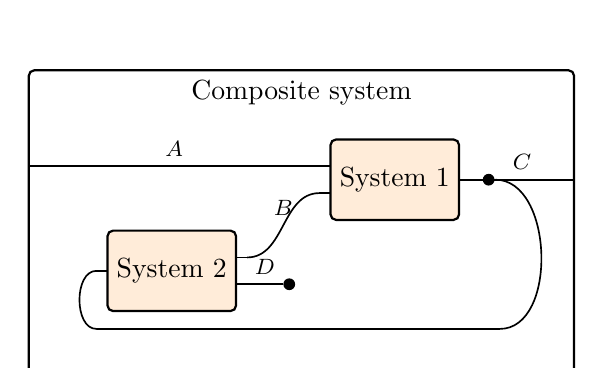
\begin{tikzpicture}[oriented WD, baseline=(B)]
        \node[bb={2}{1}, fill=orange!15] (sys1) {\text{System 1}};
        \node[bb={1}{2}, below left=0.6 and .8 of sys1, fill=orange!15]  (sys2) {\text{System 2}};
        \node[circle, inner sep=1.5pt, fill=black, right=.1] at (sys1_out1) (pdot) {};
        \node[circle, inner sep=1.5pt, fill=black, right=.3] at (sys2_out2) (wdot) {};
        \node[bb={0}{0}, inner ysep=25pt, inner xsep=1cm, fit=(sys1) (pdot) (wdot) (sys2)] (outer) {};
        \coordinate (outer_out1) at (outer.east|-sys1_out1);
        \coordinate (outer_in1) at (outer.west|-sys1_in1);
        \begin{scope}[above, font=\footnotesize]
          \draw (outer_in1) -- node {$A$} (sys1_in1);
          \draw (sys2_out1) to node (B) {$B$} (sys1_in2);
          \draw (sys2_out2) to node (X) {$D$} (wdot);
          \draw (sys1_out1) to node {$C$} (outer_out1);
          \draw
              let 
                  \p1 = (sys2.south west-| pdot),
                  \p2 = (sys2.south west),
                  \n1 = \bby,
                  \n2 = \bbportlen
              in
                  (pdot) to[out=0, in=0]
                  (\x1+\n2, \y1-\n1) --
                  (\x2-\n2, \y2-\n1) to[out=180, in=180]
                  (sys2_in1);
            \end{scope}
        \node[below=0of outer.north] {\text{Composite system}};
    \end{tikzpicture}
    \end{equation}

$A$, $B$, $C$ and $D$ here all abstractly represent sets/types. The wires do not have just any quantity flowing through them, but instead a specific kind of information. The outer system here arises out of a specific combination of the inner systems. An important fact about wiring patterns like the one above is that they give morphisms in \textbf{Poly}, while boxes give objects. This connection will be explored more deeply now.

\section{Polynomial functors in dynamical systems}

The three main objects of our study - polynomials, lenses and charts - have important roles in the study of dynamical systems, and the formalized categorical structures do as well, especially the parallel product $\otimes$. 

\subsection{Polynomials as interfaces}

A polynomial can be seen as the interface or "API" of a dynamical system, by describing what its outputs and inputs are - the outputs are the set of positions, while the inputs correspond to directions at a particular position. The simplest way to visualize a polynomial as an interface is in the case of the monomial. Consider the monomial $r$, whose interface uses familiar types. $r(y) = \texttt{(IO Int)}y^{\top}$. As a box in the wiring diagram scheme, this corresponds to:


\begin{equation}\label{eqn.control_diag}
    \begin{tikzpicture}[oriented WD, baseline=(B)]
        \node[bb={1}{1}, fill=orange!15] (sys1) {\text{$r$}};
        \node[circle, fill=white, left=1] at (sys1_in1) (invis1) {};
        \node[circle, fill=white, right=1] at (sys1_out1) (invis2) {};
        \begin{scope}[above, font=\footnotesize]
            \draw (invis1) to node {$\top$} (sys1_in1);
            \draw (invis2) to node {\texttt{IO Int}} (sys1_out1);
        \end{scope}
    \end{tikzpicture}
\end{equation}

This is a straightforward view of an interface, because monomials cannot represent mode-dependence; that is, the types of outputs and inputs to a box like the one above cannot change, no matter what the state of a machine that implements this box is. If we consider a polynomial with different sets of summands however, the situation changes. Take the polynomial below for instance.
$$
p(y) = \mathbb{R}y^{\texttt{string}} + \top y^{\mathbb{N} \times \mathbb{N}}
$$
As an interface to an abstract system, it applies to any system that, when its state is such that it outputs real numbers, the possible inputs are strings. When its state is such that it is outputting $\top$ (the singleton set), then the possible inputs to give it are pairs of natural numbers. Notice that this says nothing about what the state space of a system should concretely be, only that its state can specify its interface. Mode-dependence makes it so that writing a polynomial as an abstract box in a wiring diagram is hard, because the input and output wires change. Consider the polynomial above. There are two possible boxes that it corresponds to, depending on its state. One of them looks like this:

\begin{equation}\label{eqn.control_diag}
    \begin{tikzpicture}[oriented WD, baseline=(B)]
        \node[bb={1}{1}, fill=orange!15] (sys1) {\text{$r$}};
        \node[circle, fill=white, left=1] at (sys1_in1) (invis1) {};
        \node[circle, fill=white, right=1] at (sys1_out1) (invis2) {};
        \begin{scope}[above, font=\footnotesize]
            \draw (invis1) to node {\texttt{string}} (sys1_in1);
            \draw (invis2) to node {$\mathbb{R}$} (sys1_out1);
        \end{scope}
    \end{tikzpicture}
\end{equation}

And the second looks like this:

\begin{equation}\label{eqn.control_diag}
    \begin{tikzpicture}[oriented WD, baseline=(B)]
        \node[bb={2}{1}, fill=orange!15] (sys1) {\text{$r$}};
        \node[circle, fill=white, left=1] at (sys1_in1) (invis1) {};
        \node[circle, fill=white, left=1] at (sys1_in2) (invis3) {};
        \node[circle, fill=white, right=1] at (sys1_out1) (invis2) {};
        \begin{scope}[above, font=\footnotesize]
            \draw (invis1) to node {$\mathbb{N}$} (sys1_in1);
            \draw (invis3) to node [below] {$\mathbb{N}$} (sys1_in2);
            \draw (invis2) to node {$\top$} (sys1_out1);
        \end{scope}
    \end{tikzpicture}
\end{equation}

A good way of integrating this mode dependence inherent to polynomials into regular wiring diagrams is an open problem. Because of this, most wiring diagrams we will show are of non-mode dependent systems, and as such they represent only a small portion of the dynamical systems that \textbf{Poly} has the power to model.

\subsection{The parallel product $\otimes$}
We come to a great motivating factor for the naming of this structure: it corresponds to putting systems in parallel. Given two polynomials $p$ and $q$ with their own interfaces, taking their parallel product $p \otimes q$ corresponds to creating a polynomial that has \textit{both interfaces simultaneously}. Intuitively, one can think that any system that has this interface can only run one timestep upon being given both inputs, and it will output both outputs. The structure, in some sense, does not "touch" the behavior of the systems at all. This is represented in the below picture, by considering $p(y) = Dy^{(A \times B)}$ and $q(y) = (E \times F)y^C$: 

\begin{equation}\label{eqn.control_diag}
    \begin{tikzpicture}[oriented WD, baseline=(B)]
        \node[bb={2}{1}, fill=orange!15] (sys1) {$p$};
        \node[bb={1}{2}, below=1 of sys1, fill=orange!15]  (sys2) {$q$};
        \node[dashed, bb={0}{0}, inner ysep=25pt, inner xsep=1cm, fit=(sys1) (sys2)] (outer) {};
        \coordinate (outer_out1) at (outer.east|-sys1_out1);
        \coordinate (outer_out2) at (outer.east|-sys2_out1);
        \coordinate (outer_out3) at (outer.east|-sys2_out2);
        \coordinate (outer_in1) at (outer.west|-sys1_in1);
        \coordinate (outer_in2) at (outer.west|-sys1_in2);
        \coordinate (outer_in3) at (outer.west|-sys2_in1);
        \draw (outer_in1) -- node[above] {$A$} (sys1_in1);
        \draw (outer_in2) -- node[below] {$B$} (sys1_in2);
        \draw (outer_in3) -- node[below] {$C$} (sys2_in1);
        \draw (sys1_out1) to node[above] {$D$} (outer_out1);
        \draw (sys2_out1) to node[above] {$E$} (outer_out2);
        \draw (sys2_out2) to node[below] {$F$} (outer_out3);
        \node[below=0of outer.north] {$p \otimes q$};
    \end{tikzpicture}
    \end{equation}

The resulting polynomial functor is the dashed line around the two inner boxes, and is given by $p \otimes q(y) = DEFy^{ABC}$. The parallel product also has an important implication for the behavior of systems, as explained next.

\subsection{Lenses as behaviors}

A particular kind of lens specifies behaviors/dynamics of systems, namely any lens of shape $f : Sy^S \rightarrow p$, where $p$ is any polynomial and $S$ is the state space set. Since lenses are maps on positions and on directions, in this case we get $f : S \rightarrow p(1)$; and $f\# : (\texttt{curState}: S) \rightarrow A (\texttt{f curState}) \rightarrow S$. This corresponds to our definition of open systems, with the added mode dependence: the map on positions is exactly the \texttt{readout} function, and the map on directions is the \texttt{update} function with the added constraint that not any $A$ is valid - $A$ is now a type family, so only the fibrations of $A$ at the position (output) at the current state are valid.

A value of the type of lenses $f : Sy^S \rightarrow p$ can therefore be seen as a concrete dynamical system. At the end of the day, it is "only" a pair of functions: one to read out the exposed state of the system, and one to update the state of the system with some input. The way we will show behavior-specifying lenses in wiring diagrams is like the polynomials that represent their interfaces, but with the state space type denoted on the bottom like so:

\begin{equation}\label{eqn.control_diag}
    \begin{tikzpicture}[oriented WD, baseline=(B)]
        \node[bb={1}{1}, inner sep=25pt, fill=orange!15] (sys1) {\text{$r$}};
        \node[circle, fill=white, left=1] at (sys1_in1) (invis1) {};
        \node[circle, fill=white, right=1] at (sys1_out1) (invis2) {};
        \begin{scope}[above, font=\footnotesize]
            \draw (invis1) to node {$\mathbb{R}$} (sys1_in1);
            \draw (invis2) to node {\texttt{string}} (sys1_out1);
        \end{scope}
        \node[above right=0 and 0.3 of sys1.south] {$\mathbb{N}$};
    \end{tikzpicture}
\end{equation}


This can then be seen as a lens of type $S^S \rightarrow r$, where $S = \mathbb{N}$ and $r(y) = \texttt{string}y^{\mathbb{R}}$. Note that there are many values of this type, which is to say many ways to implement a dynamical system with this state space and this interface.

\subsection{Lenses as wiring patterns}

The other role that lenses play in systems of this kind is that they correspond to wiring patterns. For example, consider the wiring diagram below:

\begin{equation}\label{eqn.control_diag}
    \begin{tikzpicture}[oriented WD, baseline=(B)]
        \node[bb={1}{2}, fill=orange!15] (p) {\text{p}};
        \node[bb={2}{1}, below=.8 of p, fill=orange!15]  (q) {\text{q}};
        \node[circle, inner sep=1.5pt, fill=black, right=.1] at (p_out2) (pdot) {};
        \node[circle, inner sep=1.5pt, fill=black, right=.1] at (q_out1) (wdot) {};
        \node[dashed, bb={0}{0}, inner ysep=4pt, inner xsep=4pt, fit=(p) (q)]  (ptensorq) {};
        \node[bb={0}{0}, inner ysep=25pt, inner xsep=1cm, fit=(p) (pdot) (wdot) (q)] (outer) {};
        \coordinate (outer_out1) at (outer.east);
        \coordinate (outer_in1) at (outer.west|-p_in1);
        \coordinate (outer_in2) at (outer.west|-q_in1);
        \coordinate (outer_in3) at (outer.west|-q_in2);
        \begin{scope}[above, font=\footnotesize]
          \draw (outer_in1) -- node {$A$} (p_in1);
          \draw (outer_in2) -- node {$B$} (q_in1);
          \draw (outer_in3) -- node [below] {$C$} (q_in2);
          \draw (p_out1) to node {$A$} (outer_out1);
          \draw (p_out2) to node [below] {$B$} (pdot);
          \draw (q_out1) to node {$C$} (wdot);
        \end{scope}
        \node[above=0 of ptensorq.north] {$p \otimes q$};
        \node[above=0 of outer.north] {$Ay^{ABC}$};
    \end{tikzpicture}
\end{equation}

This corresponds to a lens from an abstract polynomial of the dashed box to the abstract polynomial of the outermost box. The inner dashed box is the polynomial obtained by taking the parallel product of $p$ and $q$. We say "abstract" because we need to know nothing about the dynamics or concrete behavior of the systems here, all we need is the types of the interfaces to match, which means this particular lens is capable of wiring together \textit{any} two systems that have the interfaces in question. There are of course other ways to wire these boxes together. Here are two examples:
\[
    \begin{tikzpicture}
    \node (wiring1) {
        \begin{tikzpicture}[oriented WD, baseline=(B)]
            \node[bb={1}{2}, fill=orange!15] (p) {\text{p}};
            \node[bb={2}{1}, below=2 of p, fill=orange!15]  (q) {\text{q}};
            \node[dashed, bb={0}{0}, inner ysep=4pt, inner xsep=4pt, fit=(p) (q)]  (ptensorq) {};
            \node[bb={0}{0}, inner ysep=25pt, inner xsep=1cm, fit=(p) (pdot) (wdot) (q)] (outer) {};
            \coordinate (outer_out1) at (outer.east|-p_out1);
            \coordinate (outer_in1) at (outer.west|-p_in1);
            \coordinate (outer_in2) at (outer.west|-q_in1);
            \coordinate (outer_in3) at (outer.west|-q_in2);
            \node[circle, inner sep=1.5pt, fill=black, right=.2] at (outer_in1) (adot) {};
            \node[circle, inner sep=1.5pt, fill=black, right=.2] at (p_out1) (adot2) {};
            \node[circle, inner sep=1.5pt, fill=black, right=.3] at (p_out2) (bdot) {};
            \node[circle, inner sep=1.5pt, fill=black, right=.2] at (outer_in3) (cdot) {};
            \node[circle, inner sep=1.5pt, fill=white, right=.15] at (q_out1) (qdot) {$C$};
            \begin{scope}[above, font=\footnotesize]
                \draw (outer_in1) to node {$A$} (adot);
                \draw (outer_in3) to node [below] {$C$} (cdot);
                
                \draw
                let 
                    \p1 = (p.north west-| adot2),
                    \p2 = (p.north west),
                    \n1 = \bby,
                    \n2 = \bbportlen
                in
                    (adot2) to[out=0, in=0]
                    (\x1+\n2, \y1+\n1) --
                    (\x2-\n2, \y2+\n1) to[out=180, in=180]
                    (p_in1);
                
                \draw (p_out2) to node [below] {$B$} (bdot);
                \draw (p_out1) to node {} (adot2);
                \draw (adot2) -- node {$A$} (outer_out1);
                \draw (p_out2) to node [below] {$B$} (bdot);
                
                \draw (outer_in2) to node [above] {$B$} (q_in1);
                \draw
                let 
                    \p1 = (q.south west-| q_out1),
                    \p2 = (q.south west),
                    \n1 = \bby,
                    \n2 = \bbportlen
                in
                    (q_out1) to[out=0, in=0]
                    (\x1+\n2, \y1-\n1) --
                    (\x2-\n2, \y2-\n1) to[out=180, in=180]
                    (q_in2);
            \end{scope}
    \end{tikzpicture}
    };
    %
    \node (wiring2) [right=1 of wiring1] {
        \begin{tikzpicture}[oriented WD, baseline=(B)]
            \node[bb={1}{2}, fill=orange!15] (p) {\text{p}};
            \node[bb={2}{1}, below=2 of p, fill=orange!15]  (q) {\text{q}};
            \node[dashed, bb={0}{0}, inner ysep=4pt, inner xsep=4pt, fit=(p) (q)]  (ptensorq) {};
            \node[bb={0}{0}, inner ysep=25pt, inner xsep=1cm, fit=(p) (pdot) (wdot) (q)] (outer) {};
            \coordinate (outer_out1) at (outer.east|-p_out1);
            \coordinate (outer_in1) at (outer.west|-p_in1);
            \coordinate (outer_in2) at (outer.west|-q_in1);
            \coordinate (outer_in3) at (outer.west|-q_in2);
            \node[circle, inner sep=1.5pt, fill=black, right=.3] at (p_out2) (bdot) {};
            \node[circle, inner sep=1.5pt, fill=black, right=.2] at (outer_in3) (cdot) {};
            \node[circle, inner sep=1.5pt, fill=white, right=.15] at (q_out1) (qdot) {$C$};
            \begin{scope}[above, font=\footnotesize]
                \draw (outer_in1) to node {$A$} (p_in1);
                \draw (outer_in3) to node [below] {$C$} (cdot);
                
                \draw (p_out2) to node [below] {$B$} (bdot);
                \draw (p_out1) to node {} (outer_out1);
                \draw (adot2) -- node {$A$} (outer_out1);
                \draw (p_out2) to node [below] {$B$} (bdot);
                
                \draw (outer_in2) to node [above] {$B$} (q_in1);
                \draw
                let 
                    \p1 = (q.south west-| q_out1),
                    \p2 = (q.south west),
                    \n1 = \bby,
                    \n2 = \bbportlen
                in
                    (q_out1) to[out=0, in=0]
                    (\x1+\n2, \y1-\n1) --
                    (\x2-\n2, \y2-\n1) to[out=180, in=180]
                    (q_in2);
            \end{scope}
        \end{tikzpicture}
    };
\end{tikzpicture}
\]
And they all correspond to different lenses. The intuition for the lens structure is that the map on positions selects which of the outer outputs will be served by the inner outputs, and the map on directions will fill in the needed inputs to the inner boxes. Although sometimes lenses will feed an output of a system to itself, as above, a lens is still a morphism from some inner box (here the polynomial $p \otimes q(y) = ABCy^{ABC}$) to an outer one (here the polynomial $Ay^{ABC}$).

\subsection{Commuting squares as system transformations}
Commuting squares have a deep interpretation in this context: they correspond to how behaviour can transfer between different dynamical systems.
Special kinds of commuting squares correspond to different kinds of behavior.
For example, one behavior is for one system to simulate another system, this can be encoded by a simple kind of commuting square consisting of a function between the states of the two different systems.
Two examples of such commuting diagrams are given in sections \ref{section:flipflop} and \ref{section:simulatestatemachine}.

The fact that commuting squares compose also means that behaviour compose.
For example, if system A simulates system B, and system B simulates system C, then system A simulates system C. 

%Charts also have a deep interpretation in this context: it turns out that they correspond to how behaviour can transfers between dynamical systems.
%Different kind of charts   \todo{write up charts a bit}. % We give an implementation of the example given by David Jaz in his YouTube guest lecture for the polynomial functors course.

\section{Implementing dynamical systems}

Although dynamical systems are "just" lenses of a certain form, we choose a convenient representation for them so as to align with our thinking, analogously to how we choose to represent lenses, charts and polynomials as records and not $\Sigma$-types. Some of this code is directly translated from the Idris-based implementation in the poly-book's github repository. Our characterization is the following record:
\begin{minted}{agda}
record DynamicalSystem : Set₁ where
    constructor mkdyn
    field
        state : Set -- S
        interface : Polynomial -- p
        dynamics : Lens (selfMonomial state) interface -- Sy^S → p
\end{minted}

When it comes to implementing a framework for coding up dynamical systems in this context, some patterns appear over and over. Some of these patterns are: 
\begin{itemize}
    \item Transforming a pure function $f : A \rightarrow B$ into a memoryless dynamical system, i.e. one that has $A$ as an input, $B$ as output, $A$ as a state space and whose dynamics are given by running the function $f$ on \texttt{readout} and just replace the state with the input in \texttt{update}.

        \begin{minted}{agda}
functionToDynamicalSystem : (A B : Set) → (A → B) → DynamicalSystem
functionToDynamicalSystem A B f = 
  mkdyn B (monomial B A) (id ⇆ (\_ → f))
\end{minted}
    \item Create an \texttt{emitter} polynomial that represents an interface of no inputs (i.e. takes the singleton set) and always outputs the same type.
        \begin{minted}{agda}
emitter : Set → Polynomial
emitter = linear
\end{minted}
    It should not be surprising that this is just the linear polynomial; we give it a special name to bind it to the current interpretation, in the spirit of \textit{concepts with an attitude} \cite{conceptwithattitude}.
    \item Create a \texttt{haltingEmitter} polynomial that represents an interface of a system that must halt upon outputting its left side type.
        \begin{minted}{agda}
haltingEmitter : (A B : Set) → Polynomial
haltingEmitter A B = mkpoly (A ⊎ B) halting
    where halting : {A B : Set} → (A ⊎ B) → Set
          halting (inj₁ _) = ⊥
          halting (inj₂ _) = ⊤
\end{minted}
    A system inside this interface takes no inputs in a different, more strict sense: it is not that it does not receive any outside information, like the \texttt{emitter}, but rather that any use of it must account for the case when an input cannot be produce.
    \item Taking the parallel product of two systems. Recall that the parallel product is an operation on objects (polynomials) but it also it is also possible to construct a canonical lens from two lenses $f : A \rightarrow C$ and $g : B \rightarrow D$ of type $\langle f \otimes g \rangle : A \otimes B \rightarrow C \otimes D$. In the context of systems \textit{being} morphisms, this corresponds to putting them "in parallel" and giving rise to a new system, with both state spaces, interfaces and behaviors simultaneously.
    \begin{minted}{agda}
_&&&_ : DynamicalSystem → DynamicalSystem → DynamicalSystem
mkdyn stateA interfaceA dynamicsA &&& mkdyn stateB interfaceB dynamicsB 
    = mkdyn (stateA × stateB)
            (interfaceA ⊗ interfaceB) 
            ⟨ dynamicsA ⊗ dynamicsB ⟩

\end{minted}


    \item Plugging dynamics and wiring patterns together. If lenses account both for dynamics \textit{and} wiring patterns, then it seems natural that a dynamical system (really a lens) that just contains several "free-floating" boxes that are simply sitting in parallel could be composed with a lens that represents a wiring pattern to give rise to a system that is actually usable. Indeed, this is the case, and the function that does this is called \texttt{install} by both us and the poly example code:
    \begin{minted}{agda}
install : (d : DynamicalSystem) → 
          (p : Polynomial) → 
          Lens (DynamicalSystem.interface d) p → 
          DynamicalSystem
install d p l = mkdyn (DynamicalSystem.state d)
                      p 
                      (l ∘ₚ (DynamicalSystem.dynamics d))
\end{minted}
    \item Outer box lens representations. An outer box that represents an enclosure, as well as enclosures of a couple different possible inputs are given: we use \texttt{auto} for most systems, since we are interested in just running them as closed systems and seeing what happens, but sometimes we are interested in giving constant inputs that come from outside the environment, and for that we use \texttt{constI}:
\begin{minted}{agda}
encloseFunction : {t u : Set} → (t → u) → Lens (monomial t u) Y
encloseFunction f = (λ _ → tt) ⇆ (λ fromPos _ → f fromPos)

auto : {m : Set} → enclose (emitter m)
auto = encloseFunction λ _ → tt

constI : {m : Set} → (i : m) → enclose (selfMonomial m)
constI i = encloseFunction λ _ → i
\end{minted}
    One can easily imagine extending \texttt{constI} to taking a function that operates on the number of timesteps so as to vary the input over time as well. This is something that is done in dynamical systems theory in a very informal capacity, under the intuition that the parameters of the system vary "slowly" with respect to the timescale of the state updates. With this framework, we gain the ability of making it precise for free. Of course, if we wanted to make the parameter variation respond to the system's dynamics, we would need to make it a system in itself; this is a design consideration that we hope future developers take into account. We take a mix of these two approaches for example \ref{section:hh}.
    \item Finally, there is a function that does what one accustomed to dynamical systems simulations would expect: given an abstract representation of a dynamical system (a value of type \texttt{DynamicalSystem} in our case), and an initial condition, it produces an infinite stream of outputs.
\begin{minted}{agda}
{-# TERMINATING #-}
run : (d : DynamicalSystem) → 
      enclose (DynamicalSystem.interface d) → 
      DynamicalSystem.state d → 
      Stream (Polynomial.position (DynamicalSystem.interface d)) _
run d e initialState =  [ output ] ++ (run d e next)
    where
        output : Polynomial.position (DynamicalSystem.interface d)
        output = Lens.mapPosition (DynamicalSystem.dynamics d) 
                                  initialState
        next : DynamicalSystem.state d
        next = Lens.mapDirection (DynamicalSystem.dynamics d) 
                                 initialState
                                 (Lens.mapDirection e output tt)
\end{minted}
    We need the Agda pragma \texttt{TERMINATING} here because the termination checker cannot be sure that this code terminates, since \texttt{run} calls itself on input that is not guaranteed to be smaller. We can then \texttt{take} on the resulting stream to produce regular Agda lists or vectors, and use them to render plots or print to the screen, and as long as we always run this in the context of a finite \texttt{take} call, the program should always terminate.
\end{itemize}
There are more helpers and utilities peppered throughout the code, but this is the basic glue needed to work with \textbf{Poly} in the context of dynamical systems, as the examples will demonstrate.


\subsection{Examples: Discrete systems}

We split the example implementations in the class of discrete- and continuous-time. As mentioned previously, all examples are in the strict sense discrete; the continuous ones are simply discretized with some $dt$. However, the split is still valid if one considers the spirit of the implementations.

\subsubsection{Fibonacci}
We start with the most basic example of all: a Fibonacci sequence generator implemented as a dynamical system in \textbf{Poly}. The wiring diagram of this system is as follows:

\begin{equation}\label{eqn.control_diag}
    \begin{tikzpicture}[oriented WD, baseline=(B)]
        \node[bb={2}{1}, inner sep=20pt, fill=orange!15] (plus) {$+$};
        \node[bb={1}{1}, inner sep=18pt, below=2 of plus, fill=orange!15]  (id) {\texttt{id}};
        \node[circle, inner sep=1.5pt, fill=black, right=.1] at (plus_out1) (plusdot) {};
        \node[circle, inner sep=1.5pt, fill=black, right=.1] at (id_out1) (iddot) {};
        \node[bb={0}{0}, inner ysep=20pt, inner xsep=1cm, fit=(plus) (id) (plusdot) (iddot)] (outer) {};
        \node[above right=0 and 0.22 of plus.south] {$\mathbb{N}$};
        \node[above right=0 and 0.22 of id.south] {$\mathbb{N}$};
        \node[font=\small, right=0.05 of plus_in1] {$\mathbb{N}$};
        \node[font=\small, right=0.05 of plus_in2] {$\mathbb{N}$};
        \node[font=\small, right=0.05 of id_in1]   {$\mathbb{N}$};
        \node[above=0.05 of plusdot] {$\mathbb{N}$};
        \coordinate (outer_out1) at (outer.east|-id_out1);
        \begin{scope}[above, font=\footnotesize]
            \draw (id_out1) to node [below] {$\mathbb{N}$} (outer_out1);
            \draw (plus_out1) to node {} (plusdot);
            \draw
            let 
                \p1 = (plus.south west-| plus_out1),
                \p2 = (plus.south west),
                \n1 = \bby,
                \n2 = \bbportlen
            in
                (plusdot) to[out=0, in=0]
                (\x1+\n2, \y1-\n1-\bbportlen) --
                (\x2-\n2, \y2-\n1-\bbportlen) to[out=180, in=180]
                (id_in1);
            \draw
                let 
                    \p1 = (id.north west-| id_out1),
                    \p2 = (id.north west),
                    \n1 = \bby,
                    \n2 = \bbportlen
                in
                    (iddot) to[out=0, in=0]
                    (\x1+\n2, \y1+\n1+\bbportlen) --
                    (\x2-\n2, \y2+\n1+\bbportlen) to[out=180, in=180]
                    (plus_in2);
            \draw
            let 
                \p1 = (plus.north west-| plus_out1),
                \p2 = (plus.north west),
                \n1 = \bby,
                \n2 = \bbportlen
            in
                (plusdot) to[out=0, in=0]
                (\x1+\n2, \y1+\n1) --
                (\x2-\n2, \y2+\n1) to[out=180, in=180]
                (plus_in1);
        \end{scope}
    \end{tikzpicture}
\end{equation}

To break it down: the $+$ function takes two natural numbers and produces one output, and the $id$ function takes a natural number and outputs a natural number. In terms of dynamical systems, however, we have to think about what the \texttt{readout} and \texttt{update} functions are doing for each system: \texttt{readout} can only read what the current state is, and \texttt{update} can only update the state given an input. At every timestep, all systems produce their outputs based on the current state, then all the inputs are read, and the states of all systems are updated. Therefore, the effect of the \texttt{id} function is only felt one timestep later. Hence it plays the subtle role of storing the Fibonacci value computed in the previous timestep, which is why its output is fed as an input to the $+$ function. The code for this system is this:

\begin{minted}[escapeinside=||]{agda}
delay : (A : Set) → DynamicalSystem
delay A = functionToDynamicalSystem A A id

plus : DynamicalSystem
plus = functionToDynamicalSystem (Nat × Nat) Nat (uncurry _+ℕ_)

prefib : DynamicalSystem
prefib = plus &&& delay Nat

fibWiringDiagram : Lens (interface prefib) (emitter Nat)
fibWiringDiagram = (λ {(sumOutput , idOutput) → idOutput})
                    ⇆ 
                    (λ {(sumOutput , idOutput) _ → 
                            (idOutput , sumOutput) , sumOutput })

fibonacci : DynamicalSystem
fibonacci = install prefib (emitter Nat) fibWiringDiagram
\end{minted}

This example provides a good opportunity to understand dynamical systems in the context of polynomials, so let us take the chance to dig in further. In keeping with the previously mentioned intuition, the \texttt{fibWiringDiagram} lens is just one of many possible wiring patterns for an emitter-enclosed system that contains two "floating" dynamical systems that have the interfaces of \texttt{plus} and \texttt{delay Nat}. The outer outputs are the target of the lens, so the polynomial \texttt{emitter Nat}, which is a polynomial that takes the singleton set as input and outputs natural numbers. The inner inputs are given by the wiring pattern in the lens, specifically in the second function (the map on directions). This part of the code:
\begin{minted}{agda}
(λ {(sumOutput , idOutput) _ → 
    (idOutput , sumOutput) , sumOutput })
\end{minted}
is, on the right hand side, saying that the two inputs to \texttt{plus} are given by the output of \texttt{delay Nat} and the its own output, named \texttt{idOutput} and \texttt{sumOutput} respectively in the lambda. The input to \texttt{delay Nat}, on the other hand, is given by the output of the sum: in the next time step, this value will appear in the variable \texttt{idOutput}.

Two final remarks about the Fibonacci sequence generator: the first is that it is actually an efficient way to express Fibonacci dynamics, since there is no recursive calls involved - and the second is that we went into as much detail as possible explaining it so that we can rely on some of the intuition built here to explain the more complicated systems that follow.

\subsubsection{Flip Flop}\label{section:flipflop}
Flip Flop is a simple example with two dynamical systems showing how one system can simulate the behavior of another system. This simulation is exactly a special kind of commuting square between charts and lenses. 

Both systems needs to have the same interface, which in this case is a linear polynomial \texttt{\{on, off\}}$y$, that can output either on or off, and always takes unit as input. However, the state and the behavior of the systems can differ. One of the systems is a flip flop system, with states on or off, with behaviour that outputs this state, and flips the state in the update. The other system has natural numbers as states, outputs the two different states depending on the natural number modulus 2, and updates the state by always taking the successor of the state. Running these systems has the exact same output. This can be expressed concisely by a chart transforming the state space of the natural numbers to either on or off. Then by putting this chart in a commuting square such as shown in diagram \ref{fig:flipFlopSquare}.

\begin{minted}{agda}
data Switch : Set where
    on : Switch
    off : Switch

toggle : Switch → Switch
toggle on = off
toggle off = on

-- | Commonly used where input to enclosed dynamical system where
--   updateState only depends on current state.
ignoreUnitInput : {A B : Set} → (A → B) → A → ⊤ → B
ignoreUnitInput f a tt = f a

-- | Note: linear interface is used to accept only 1 possible input.
--   Readout defined as id to expose state.
flipFlop : DynamicalSystem
flipFlop = mkdyn Switch (linear Switch) (id ⇆ ignoreUnitInput toggle)

-- | Result is: on, off, on, off...
flipFlopRan : Vec Switch 10
flipFlopRan = take 10 $ run flipFlop auto on

modNat : Nat → Switch
modNat n = if n % 2 == 0 then on else off

-- | To compare flipFlop and counter they need to have the same interface.
counter : DynamicalSystem
counter = mkdyn Nat (linear Switch) (modNat ⇆ ignoreUnitInput suc)

-- | Result is: on, off, on, off...
counterRan : Vec Switch 10
counterRan = take 10 $ run counter auto 0

-- | Morphism between p dynamicalSystems with states Nat and Switch.
morphSystem : Nat → Switch
morphSystem = modNat

-- | The square expressing the simulation.
square : LensChartCommute (dynamics counter)
                          (dynamics flipFlop) 
                          (morphSystem ⇉ λ _ → morphSystem)
                          idChart
square = law₁ , law₂
\end{minted}



\begin{figure}[H]

% https://q.uiver.app/?q=WzAsNSxbMCwwLCJOeV4xIl0sWzMsMCwiMnleMSJdLFswLDMsIjJ5XjEiXSxbMywzLCIyeV4xIl0sWzYsMF0sWzAsMiwiXFwlIDIiLDIseyJvZmZzZXQiOjJ9XSxbMiwwLCJzdWMiLDIseyJvZmZzZXQiOjJ9XSxbMSwzLCJpZCIsMix7Im9mZnNldCI6Mn1dLFszLDEsInRvZ2dsZSIsMix7Im9mZnNldCI6Mn1dLFsyLDMsImlkX3tjaGFydH0iLDFdLFswLDEsIlxcJSAyIiwxLHsib2Zmc2V0IjotMn1dLFswLDEsIlxcJTIiLDEseyJvZmZzZXQiOjJ9XV0=
\[\begin{tikzcd}
	{Ny^1} &&& {2y^1} &&& {} \\
	\\
	\\
	{2y^1} &&& {2y^1}
	\arrow["{\% 2}"', shift right=2, from=1-1, to=4-1]
	\arrow["suc"', shift right=2, from=4-1, to=1-1]
	\arrow["id"', shift right=2, from=1-4, to=4-4]
	\arrow["toggle"', shift right=2, from=4-4, to=1-4]
	\arrow["{id_{chart}}"{description}, from=4-1, to=4-4]
	\arrow["{\% 2}"{description}, shift left=2, from=1-1, to=1-4]
	\arrow["{\%2}"{description}, shift right=2, from=1-1, to=1-4]
\end{tikzcd}\]

    \caption{A special kind of commuting square. The identity chart turns this into a commuting triangle. The chart at the top is defined as the function reducing the states between the systems. The laws are fulfilled if this diagram commuting encodes what it means for a system to simulate another.}
    \label{fig:flipFlopSquare}

\end{figure}

This showcased how a simple chart in a commuting square can compare behaviour of two different dynamical systems. By generalizing, and using more advanced charts and commuting squares, more advanced comparisons can be made.

\subsubsection{Simulating state machines}\label{section:simulatestatemachine}
A more advanced example, in comparison to flip flop, is how one state machine can simulate another. This is often expressed as that one state machine is more minimal than another, that is, it has less states but achieves the same behaviour. This is exactly what the special commuting square can express. Because the same idea is followed as for the flip flop example, this example will not be discussed further, but can be found in \texttt{Dynamical/Chart/SimulateStateMachine.agda}.

\subsubsection{Moore machine}
A Moore machine is the same as a lens to a monomial. A Moore machine can be defined as:

\begin{minted}{agda}
record MooreMachine {State Input Output : Set} : Set where
    constructor mkMooreMachine
    field
        readout : State → Output
        update : State → Input → State
\end{minted}

Since a moore machine is a polynomial, it is possible to define the dynamical system as a moore machine and then transport it into a lens, or the other way around.

\subsubsection{Deterministic finite automaton}
A deterministic finite state automaton (DFA) is also a special kind of lens, the lens to the monomial $2y^{alphabet}$. A DFA can be defined as:
\begin{minted}{agda}
record DFS {State Alphabet : Set} : Set where
    constructor mkDFS
    field
        -- Transition function
        update : State → Alphabet → State
        -- Partitions all states into recognized and unrecognized states.
        recognized : State → Bool
\end{minted}

The equality can be defined as a simple isomorphism.

The same trick as for the Moore machine can be used to provide an initial state to the DFA.


\subsubsection{Turing machines}

One of the examples given by the authors is of a Turing machine. A Turing machine consists of two components:
\begin{itemize}
    \item An infinitely long tape, indexed by integers, which: \begin{itemize}
        \item Has a notion of what its current index is.
        \item At each index, contains symbols of an alphabet set $A := \{\mathbb{0}, \mathbb{1}, \mathbb{b}\}$ 
        \item Can receive commands in an alphabet set $C := \{\leftarrow, \rightarrow\} + A$ to change its current index by $+1$ or $-1$ and or to change which symbol is at the current index.
    \end{itemize}
    \item A processor, which can:
    \begin{itemize}
        \item Output the aforementioned commands to the tape according to some internal logic that operates on a state S.
        \item Read the symbol at the tape's current index.
    \end{itemize}
\end{itemize}

These two components can be represented as dynamical systems, and then wired together to give a Turing machine, like in the wiring diagram in Figure \ref{wd:turing}.

\begin{figure}
    \[
    \begin{tikzpicture}[oriented WD, baseline=(B)]
        \node[bb={1}{1}, inner ysep=20pt, inner xsep=30, fill=orange!15] (tape) {tape};
        \node[bb={1}{1}, below=3 of tape, inner sep=20pt, fill=orange!15] (proc) {processor};
        \node[bb={0}{0}, inner ysep=20pt, inner xsep=1cm, fit=(tape) (proc)] (outer) {};
        \node[above left=0 and -0.08 of tape.south east] {$\mathbb{Z} \times \text{A}^{\mathbb{Z}}$};
        \node[above left=0 and -0.06 of proc.south east] {S};
        \node[font=\small, right=0.05 of tape_in1] {C};
        \node[font=\small, right=0.05 of proc_in1] {A};
        \begin{scope}[above, font=\footnotesize]   
            \draw
            let 
                \p1 = (tape.south west-| tape_out1),
                \p2 = (tape.south west),
                \n1 = \bby,
                \n2 = \bbportlen
            in
                (tape_out1) to[out=0, in=0]
                (\x1+\n2, \y1-\n1-\bbportlen) --
                (\x2-\n2, \y2-\n1-\bbportlen) to[out=180, in=180]
                (proc_in1);
            \draw
            let 
                \p1 = (proc.north west-| proc_out1),
                \p2 = (proc.north west),
                \n1 = \bby,
                \n2 = \bbportlen
            in
                (proc_out1) to[out=0, in=0]
                (\x1+\n2, \y1+\n1) --
                (\x2-\n2, \y2+\n1) to[out=180, in=180]
                (tape_in1);
        \end{scope}
    \end{tikzpicture}
    \]
    \caption{Turing machine as a wiring diagram. The processor issues commands and reads the tape's current index.}
    \label{wd:turing}
\end{figure}

A real Turing machine must be able to output something to the outer box, which happens once it is halted, while Figure \ref{wd:turing} only shows them while running/communicating. This is an example of mode-dependence being hard to express.

\remarktitle{Implementation outline}
We can implement the Turing machine setup above by first defining the sets used:

\begin{minted}[escapeinside=||]{agda}
data Alphabet : Set where
    |$\mathbb{0}$| |$\mathbb{1}$| 𝕓 : Alphabet

data Movement : Set where 
    𝕝 𝕣 : Movement
\end{minted}

And then defining each part of the system. Since Turing machines typically have a halting state, we represent this for the processor:
\begin{minted}{agda}
ProcessorState : Set
ProcessorState = ℕ 

data ProcessorOutput : Set where
    move : Movement → ProcessorOutput
    write : Alphabet → ProcessorOutput
    halt : ProcessorOutput

data ProcessorInput : Set where
    instruction : Alphabet → ProcessorInput

procInputFromOutput : ProcessorOutput → Set
procInputFromOutput (move x) = ProcessorInput
procInputFromOutput (write x) = ProcessorInput
procInputFromOutput halt = ⊤

processorInterface : Polynomial
processorInterface = (mkpoly ProcessorOutput procInputFromOutput)
\end{minted}

The \texttt{ProcessorState} type is a dummy type, since there will be no Turing program written, so it is fine to represent the state as a simple natural number. The \texttt{procInputFromOutput} function is capturing the idea that once the processor outputs \texttt{halt}, it accepts only a mindless input with no meaning. This could also be represented as the empty type, as in NO input, but it becomes somewhat harder to synchronize with the tape's own possible inputs, as will be demonstrated next.

Now the same is done for the tape

\begin{minted}{agda}
data TapeInput : Set where
    write : Alphabet → TapeInput
    move : Movement → TapeInput
    halt : TapeInput
    
TapeAt : Set
    TapeAt = ℤ → Alphabet
  
data TapeOutput : Set where
    goOut : Alphabet → TapeOutput
    haltOut : TapeAt → TapeOutput
  
tapeInputFromOutput : TapeOutput → Set
tapeInputFromOutput (goOut x) = TapeInput
tapeInputFromOutput (haltOut x) = ⊥
  
tapeInterface : Polynomial
tapeInterface = mkpoly TapeOutput tapeInputFromOutput

data TapeState : Set where
  go : TapeAt → TapeState
  halt : TapeAt → TapeState
\end{minted}

The tape's associated types and polynomial are more complex. There are a few things to notice.

Firstly, the tape does in fact not accept any more inputs when it is outputting a halting state. The reason it can get away with this, but not the processor, is that the processor \textit{decides} when to halt the program, and so its output of \texttt{halt} needs to reach the tape - for that, at least one more input is needed.

Second, the tape state contains \textit{only} the $\text{A}^{\mathbb{Z}}$ part of the diagram, and not the notion of which index it is at. The trick is to always consider the index to be zero, and treat the move directions as post composing the tape with an increment or decrement function. Since the tape behavior is always the same for any Turing machine, we provide it:

\begin{minted}{agda}
tapeBehavior : Lens (selfMonomial TapeState) tapeInterface
tapeBehavior = 
    readout ⇆ update
    where readout : TapeState → TapeOutput
          readout (go tapeAt) = goOut (tapeAt 0ℤ)
          readout (halt tapeAt) = haltOut tapeAt 
          update : (x : TapeState) → 
                   (tapeInputFromOutput (readout x)) → 
                   TapeState
          update (go tapeAt) (write x) = go $ λ tapeIndex → 
            if ⌊ tapeIndex ≟ 0ℤ ⌋ 
                then x 
                else tapeAt tapeIndex
          update (go tapeAt) (move x) = go (moveTape x tapeAt)
              where moveTape : Movement → TapeAt → TapeAt
                      moveTape 𝕝 f = f ∘ (1ℤ +ℤ_ )
                      moveTape 𝕣 f = f ∘ (1ℤ -ℤ_ )
          update (go tapeAt) halt = halt tapeAt
\end{minted}

The idea of postcomposing with an increment/decrement operation comes from the book's associated YouTube lectures. Finally, there is the need to parallel-productize the two systems together and then wire them, finding a suitable run-time representation for the tape state. We chose a vector that represents the indices 0-255 of it.

\begin{minted}[escapeinside=||]{agda}
tape : DynamicalSystem
tape = mkdyn TapeState tapeInterface tapeBehavior

preTuring : DynamicalSystem
preTuring = tape &&& processor

open DynamicalSystem
Word : Set
Word = Vec ℤ 256
toInt : Alphabet → ℤ
toInt |$\mathbb{0}$| = 0ℤ
toInt |$\mathbb{1}$| = 1ℤ
toInt 𝕓 = 1ℤ +ℤ 1ℤ
turingWiringDiagram : Lens (interface preTuring) (haltingEmitter Word ⊤)
turingWiringDiagram = outerOutput ⇆ fillInputs
  where outerOutput : TapeOutput × ProcessorOutput → (Word ⊎ ⊤)
        outerOutput (goOut x , procOut) = inj₂ tt
        outerOutput (haltOut x , _) = inj₁ $ 
            Data.Vec.map (toInt ∘ x) (tabulate (+_ ∘ toℕ))
        fillInputs : (fromPos : position (interface preTuring)) →
                     direction (haltingEmitter Word ⊤) 
                               (outerOutput fromPos) → 
                     direction (interface preTuring)
                               fromPos
        fillInputs (goOut tapeInstruction , move procInstruction) tt = 
            move procInstruction , instruction tapeInstruction
        fillInputs (goOut tapeInstruction , write procInstruction) tt = 
            (write procInstruction) , instruction tapeInstruction
        fillInputs (goOut _ , halt) tt = halt , tt

\end{minted}

A remarkable thing to notice about this system wiring is that \texttt{fillInputs} does not even allow us to pattern match on an invalid combination of inputs to the system, like \texttt{haltOut \_ , tt}, since it is a dependent function on the result of \texttt{outerOutput}, which guarantees a \texttt{haltOut} always maps to \texttt{inj₁} and this corresponds to no input. Dependent types allows us to make illegal states truly unrepresentable.

\subsection{Examples: Continuous systems}
Now we move on to discretized continuous-time systems. They may be treated in much more rigorous mathematical detail than we do here, by representing the state space as topological spaces or manifolds \cite{css}, but as we have mentioned, to showcase their implementation in \textbf{Poly} we discretize them simply according to a differential time $dt$ supplied by the user.
\remarktitle{Supporting Haskell code}
Unfortunately, not all the code in this thesis could be kept in Agda, since it would require too much reimplementation of basic user functionality, or would not be efficient. Therefore, there are the following accompanying tiny Haskell libraries:
\begin{itemize}
    \item A command-line interface library for running the continuous-time systems, since each of them requires different parameters, and using the \texttt{optparse-applicative} \cite{optparse} library.
    \item A plotting library, which renders each system as a collection of values of the system at a sequence of timsteps, written using the \texttt{Chart} \cite{chart-lib} library (not to be confused, of course, with the Chart arrow between polynomials).
    \item A matrix-multiplication library with a single function which takes a list-of-lists representation of a matrix and returns its pseudoinverse. This is needed for the last example. Taking the pseudoinverse of a matrix is a costly operation, and there was an attempt to do it in Agda, but the associated proofs were not trivial and the performance was prohibitively slow. Therefore, we outsource matrix inversion to the \texttt{hmatrix} \cite{hmatrix} Haskell library, which relies on underlying BLAS \cite{blas} algorithms for speed, while passing \texttt{trustMe} proofs to guarantee matrix sizes at the Agda level.
\end{itemize}
For more information on this supporting code, see the Appendix \ref{app:haskell}.
With this context, we move on the the systems in question.

\subsubsection{Lotka-Volterra}

The Lotka-Volterra predator-prey model is an essential system \cite{Murray2002} that portrays how the population of predators interacts with the population of prey in a given environment. The two main quantities in the model are two real numbers, abstractly representing the amount of the two types of animals - these are its states, in our context. The model is given by the two equations below, where $r$ and $f$ represent our populations of rabbits and foxes - our chosen species of prey and predator:
\begin{equation}
\dot{r} = \alpha r - \beta f r
\label{eq:rabbits}
\end{equation}
\begin{equation}
\dot{f} = \delta f r - \gamma f
\label{eq:foxes}
\end{equation}

The logic of it is that, for rabbits, they will reproduce naturally at a rate $\alpha$, while being hunted at a rate $\beta f$. In other words, their encounters with and subsequent predation by foxes is modeled by multiplying the number of foxes by a "fox appetite" parameter $\beta$. For foxes, their population can be thought of as flourishing or growing at the rate that they can encounter and eat rabbits. This aspect is captured by the term $\delta f r$. They naturally die at a rate of $\gamma$. Note that $\delta$ does not have to match $\beta$ - the rate at which foxes eat rabbits is not necessarily the same as the rate at which fox populations grow as a result of being well-fed, though the intuitive relationship between these parameters could be captured by a more sophisticated model.

This system can be represented in terms of our open dynamical systems by considering the rabbit and fox populations as each inhabited by an individual system. They output their population (so \texttt{readout} is the identity function) and that gets fed as an input to the other system, along with any other parameters - in this case $\alpha$, $\beta$, $\delta$ and $\gamma$. Here is the wiring diagram for it:

\begin{equation}\label{wd:lotkavolterra}
    \begin{tikzpicture}[oriented WD, baseline=(B)]
        \node[bb={2}{1}, inner sep=20pt, fill=orange!15] (r) {rabbits};
        \node[bb={2}{1}, below=3 of r, inner sep=23pt, fill=orange!15] (f) {foxes};
        \node[circle, inner sep=1.5pt, fill=black, right=.1] at (r_out1) (rdot) {};
        \node[circle, inner sep=1.5pt, fill=black, right=.1] at (f_out1) (fdot) {};
        \node[bb={0}{0}, inner ysep=20pt, inner xsep=1cm, fit=(r) (f) (rdot) (fdot)] (outer) {};
        \node[above right=0 and 0.45 of r.south] {$\mathbb{R}$};
        \node[above right=0 and 0.42 of f.south] {$\mathbb{R}$};
        \node[font=\small, right=0.05 of r_in1] {$\mathbb{R}$};
        \node[font=\small, right=0.05 of r_in2] {$\mathbb{R}$};
        \node[font=\small, right=0.05 of f_in1] {$\mathbb{R}$};
        \node[font=\small, right=0.05 of f_in2] {$\mathbb{R}$};
        \coordinate (outer_in1) at (outer.west|-r_in1);
        \coordinate (outer_in2) at (outer.west|-f_in2);
        \coordinate (outer_out1) at (outer.east|-r_out1);
        \coordinate (outer_out2) at (outer.east|-f_out1);
        \begin{scope}[above, font=\footnotesize]
            \draw node [above] {} (outer_in1) to (r_in1);
            \draw node [above] {} (outer_in2) to (f_in2);
            
            \draw (r_out1) to node [above] {$\mathbb{R}$} (outer_out1);
            \draw (f_out1) to node [below] {$\mathbb{R}$} (outer_out2);
            \draw
            let 
                \p1 = (r.south west-| r_out1),
                \p2 = (r.south west),
                \n1 = \bby,
                \n2 = \bbportlen
            in
                (rdot) to[out=0, in=0]
                (\x1+\n2, \y1-\n1-\bbportlen) --
                (\x2-\n2, \y2-\n1-\bbportlen) to[out=180, in=180]
                (f_in1);
            \draw
            let 
                \p1 = (f.north west-| f_out1),
                \p2 = (f.north west),
                \n1 = \bby,
                \n2 = \bbportlen
            in
                (fdot) to[out=0, in=0]
                (\x1+\n2, \y1+\n1) --
                (\x2-\n2, \y2+\n1) to[out=180, in=180]
                (r_in2);
            \node[draw=black, fill=white, circle, inner sep=1.2pt] (beta) at ($(r_in2) + (-0.2, -2.4)$){$\beta$};
            \node[draw=black, fill=white, circle, inner sep=2pt] (delta) at ($(f_in1) + (-0.2, 0.2)$) {$\delta$};
        \end{scope}
    \end{tikzpicture}
\end{equation}

The circles with the constants signify multiplication of the values by the constants $\beta$ and $\delta$. This is something we express at the wiring pattern lens' level in this system. 

Thinking of the systems individually allows us a "separation of concerns" in specifying these systems' behavior that is not there in environments like Matlab or Python. The code for the rabbit system is:
\begin{minted}[escapeinside=||]{agda}
rabbits : DynamicalSystem
rabbits = mkdyn |$\mathbb{ℝ}$| (mkpoly ℝ λ _ → ℝ × ℝ) (readout ⇆ update)
  where readout : ℝ → ℝ
        readout state = state
        update : ℝ → ℝ × ℝ → ℝ
        update state (birthRabbits , deathRabbits) = 
            state + dt * (state  * (birthRabbits - deathRabbits))
\end{minted}
The differential equation is directly discretized, so the differential amount of time $dt$ goes to the right hand side of \ref{eq:rabbits} and multiplies the entire thing; this is then added to the current state to produce a new state.

Similarly, the fox system is given as:
\begin{minted}{agda}
foxes : DynamicalSystem
foxes = mkdyn ℝ (mkpoly ℝ λ _ → ℝ × ℝ) (readout ⇆ update)
  where readout : ℝ → ℝ
        readout state = state
        update : ℝ → ℝ × ℝ → ℝ
        update state (birthFoxes , deathFoxes) = 
            state + dt * (state * (birthFoxes - deathFoxes))
\end{minted}

Note that each of these systems have only two parameters, whereas by the equations \ref{eq:rabbits} and \ref{eq:foxes}, they ought to have three: \ref{eq:rabbits} should get $\alpha$ and $\beta$ from "outside" the system, whereas \ref{eq:foxes} should get $\delta$ and $\gamma$. It is a somewhat arbitrary choice that we make to make the $\beta$ and $\gamma$ parameters part of the larger system, that is the one given rise to by the composition of these systems parallel-productized with the wiring diagram, and not constants within the system themselves, for instance.

The final system is then a composition with a certain wiring diagram lens:

\begin{minted}{agda}
preLV : DynamicalSystem
preLV = rabbits &&& foxes

-- Wiring diagram is an lens between monomials
lotkaVolterraWiringDiagram : ℝ → ℝ → 
    Lens (DynamicalSystem.interface preLV) (selfMonomial (ℝ × ℝ))
lotkaVolterraWiringDiagram foxPerCapDeath foxHunger = 
  outerOutput ⇆ innerInput
    where outerOutput : ℝ × ℝ → ℝ × ℝ
          outerOutput (rabbitOutput , foxOutput) = 
            rabbitOutput , foxOutput
          innerInput : (outputs : ℝ × ℝ) → 
                       direction (selfMonomial (ℝ × ℝ)) 
                                 (outerOutput outputs) →
                       direction (interface preLV) outputs
          innerInput (r , f) (rabMaxPerCapGrowth , howNutritiousRabbitsAre) = 
            (rabMaxPerCapGrowth , foxHunger * f) , 
            (foxPerCapDeath * r , howNutritiousRabbitsAre)
-- Final system is composition of wiring diagram and dynamics
lotkaVolterra : ℝ → ℝ → DynamicalSystem
lotkaVolterra β γ = install preLV 
                            (selfMonomial (ℝ × ℝ))
                            (lotkaVolterraWiringDiagram β γ)
\end{minted}

Running this system through the command line interface produces the expected oscillating dynamics of the Lotka-Volterra model, albeit with some numerical instability causing the oscillations to grow slightly. Figure \ref{fig:lvfig} shows this dynamics, obtained by running the system through the command line interface with the following parameters.

\begin{minted}{shell}
    ./Plot LotkaVolterra --alpha 0.2 --beta 0.2 --delta 0.5 \
                         --gamma 0.4 --r0 1.0 --f0 0.9 --dt 0.1
    \end{minted}

\begin{figure}[H]
    \centering
    \includegraphics[width=0.9\textwidth]{figure/lotka_volterra.png}
    \caption{Lotka-Volterra oscillatory dynamics. As the population of rabbits grows, the population of foxes catches up, causing it to go down.}
    \label{fig:lvfig}
\end{figure}


\subsubsection{Lorenz system}
The Lorenz system \cite{lorenz1963} is what is known as a chaotic system, in an elementary form. It was introduced by Edward Lorenz as a simplified model of atmospheric convection. The three dimensionless (as in, pure proportions with no physical units) variables $x$, $y$ and $z$ correspond to rate of convection, temperature difference between ascending and descending air currents, and how temperature changes with height. It is given by the following differential equations:

\begin{equation}
\dot{x} = \sigma (y - x)
\label{eq:xlor}
\end{equation}
\begin{equation}
\dot{y} = x(\rho - z) - y
\label{eq:ylor}
\end{equation}
\begin{equation}
\dot{z} = xy - \beta z
\label{eq:zlor}
\end{equation}

The system has three numeric parameters, $\sigma$, $\rho$ and $\beta$ and for specific values of these parameters ($\sigma = 10.0$, $\rho = 28.0$, $\beta = 8/3$), it displays chaotic dynamics - dynamics that have the property of becoming hard to predict as time goes on. What this means is that for two arbitrarily close initial conditions, the distance between the trajectories followed by running the system with these initial conditions grows exponentially, until the trajectories are maximally distant. Figure \ref{fig:lorenzbutterfly} shows an example trajectory of the system with the parameters mentioned above.

\begin{figure}
    \centering
    \includegraphics[width = 0.9\textwidth]{figure/lorenzbutterfly.png}
    \caption{"Lorenz butterfly", a visualization of a trajectory of the Lorenz system. $dt$ is set to 0.01.}
    \label{fig:lorenzbutterfly}
\end{figure}

This is known as a "strange attractor": the system's trajectories eternally oscillate between two attracting states, but they never converge to a single orbit, jumping back and forth. The system is a greatly simplified model of the atmosphere, but provides a good "essence" of chaotic dynamics that are hard to predict, even in just three variables. 

Implementing the Lorenz system in terms of \textbf{Poly} follows the same pattern as the Lotka-Volterra model, by capturing each equation in its own box with its own internal state, with the difference that the external parameters are now fixed, so the inputs are now only the external variables upon which each box should depend. In Agda, the systems are given as:
\begin{minted}{agda}
-- First order differential equations
x : ℝ → DynamicalSystem
x dt = mkdyn X (mkpoly X λ _ → Y) (readout ⇆ update)
  where readout : X → X
        readout state = state
        update : X → Y → X
        update (xnt state) (ynt y) = 
            xnt (state + dt * (σ * (y - state)))

y : ℝ → DynamicalSystem
y dt = mkdyn Y (mkpoly Y λ _ → X × Z) (readout ⇆ update)
  where readout : Y → Y
        readout state = state
        update : Y → X × Z → Y
        update (ynt state) ( xnt x , znt z ) = 
            ynt (state + dt * (x * (ρ - z) - state))

z : ℝ → DynamicalSystem
z dt = mkdyn Z (mkpoly Z λ _ → X × Y) (readout ⇆ update)
  where readout : Z → Z
        readout state = state
        update : Z → X × Y → Z
        update (znt state) (xnt x , ynt y) = 
            znt (state + dt * (x * y - β * state))
\end{minted}
And they are again parallel-productized, producing a system with 3 inputs and 3 outputs, then wired in the right way (x is given as an input to y and z, y to x and z, and z to y, as per the system equations)

\begin{minted}{agda}
preLorenz : ℝ → DynamicalSystem
preLorenz dt = x dt &&& y dt &&& z dt

-- Wiring diagram is an lens between monomials
lorenzWiringDiagram : Lens (interface (preLorenz _))
                           (emitter (X × Y × Z))
lorenzWiringDiagram = mp ⇆ md
  where mp : X × Y × Z → X × Y × Z
        mp (x , y , z) = x , y , z
        md : X × Y × Z → ⊤ → Y × (X × Z) × (X × Y)
        md (x , y , z) _ = y , (x , z) , (x , y)

-- Final system is composition of wiring diagram and dynamics
lorenz : ℝ → DynamicalSystem
lorenz dt = install (preLorenz dt)
                    (emitter (X × Y × Z))
                    lorenzWiringDiagram
\end{minted}

An example run of this system, obtained by \texttt{take} of 1000 timesteps at $dt = 0.01$, is given in Figure \ref{fig:lorenz_dynamics}.

\begin{figure}
    \centering
    \includegraphics[width=0.9\textwidth]{figure/lorenz_dynamics.png}
    \caption{Lorenz system chaotic dynamics. The three variables keep oscillating in ever-changing patterns, never settling to a stable cycle.}
    \label{fig:lorenz_dynamics}
\end{figure}


\subsubsection{Hodgkin-Huxley model}
\label{section:hh}
The two examples given in this section are closed systems, meaning they take no input - what this really means is that they take the singleton set as input, so each timestep the element \texttt{tt} is given as a value and the system produces the next output. Now we come to a slightly bigger and more realistic system with 4 equations: the Hodgkin-Huxley \cite{hodgkin1952quantitative} model. It is a system that models action potentials in the giant squid neuron, by thinking of the neuron membranes as circuits, so that the relevant quantities are all electrical (charge, current, capacitance etc). This model captures the flow of sodium and potassium ions through ion channels in the membrane, like in Figure \ref{fig:hodgkinhuxleyschematic}, obtained from \cite{gerstner2014neuronal}.

\begin{figure}
    \centering
    \includegraphics{figure/hodgkinhuxley.png}
    \caption{Analogy schematic of a neuronal membrane modeled as a circuit, from the book Neuronal Dynamics.}
    \label{fig:hodgkinhuxleyschematic}
\end{figure}

The interesting thing about the Hodgkin-Huxley model is that it actually lends itself to being implemented as an open system. There are several equivalent ways of formulating HH as a 4-dimensional dynamical system, but the equations we use are according to \href{https://mark-kramer.github.io/Case-Studies-Python/HH.html}{this online tutorial} by Mark Kramer and given by:

\begin{equation}
\dot{V} =  G_{na}m^3h(E_{na} - V_s) + G_kn^4(E_k - V_s) + G_L * (E_L - V_s) + I_e
\label{eq:voltage}
\end{equation}
\begin{equation}
\dot{m} = \alpha_m(V)(1.0 - m) - \beta_m(V)m
\label{eq:mhh}
\end{equation}
\begin{equation}
\dot{h} = \alpha_h(V)(1.0 - h) - \beta_h(V)h
\label{eq:hhh}
\end{equation}
\begin{equation}
\dot{n} = \alpha_n(V)(1.0 - n) - \beta_n(V)n   
\label{eq:nhh}
\end{equation}

The variables here mean the following: $V$ is the resulting voltage between the intra and extracellular mediums, $m$ encodes potassium channel activation probability, $h$ encodes sodium channel activation probability and $n$ encodes sodium channel \textit{inactivation} probability, and $I_e$ is the driven input voltage. All other symbols are constants and helper functions that have their own deep theoretical justification which we will not get into, we will just explain the basic logic of the system. The idea is that potassium and sodium channels are positively charged, so their flow across their membrane corresponds to current. However, their flow is not only affected by voltage, but also by concentration: in a chemical setting, substances can saturate a solution regardless of their charge. The interacting probabilities of channels activating (opening, thus allowing particles to flow from more to less concentrated environments) or inactivating give rise to interesting voltage dynamics - the voltage is in fact the output we are interested in for this particular application. Given a strong enough input current, the system can be made to display oscillating behavior, which corresponds to the neuron firing.

The input current can be a constant value, in which case it might as well be treated as a parameter, or an input to an open dynamical system as we have been describing in the framework we work in. This allows us to model "changing a parameter" of a dynamical system, but in a way that is totally internal to our modeling language and does not rely on ad-hoc formulations or programming \footnote{For a description of the informal process of analyzing changing a parameter as "turning a knob" at a timescale that is much bigger than the system's dynamics, see this lecture by Shane Ross on the book Nonlinear Dynamics and Chaos by Strogatz: https://www.youtube.com/watch?v=BBd68\_q3Dgg.}.

The code for the equations themselves, represented as systems, follows the same pattern as the two previous examples. It also involves many fixed constants, discovered experimentally, and so it is quite big, so for the sake of clarity we omit most of it for this system. Instead we focus on the wiring pattern, as well use of \texttt{constI} as a constant input to the system to showcase running a system:
\begin{minted}{agda}
preHH : ℝ → DynamicalSystem
preHH dt = voltage dt &&& 
           potassiumActivation dt &&& 
           sodiumActivation dt &&&
           sodiumInactivation dt

hodgkinHuxleyWiringDiagram : Lens (interface (preHH _)) (selfMonomial ℝ)
hodgkinHuxleyWiringDiagram = 
    (λ {(v , m , h , n) → v }) ⇆ 
    (λ {((v , m , h , n)) Ie → (Ie , m , h , n) , v , v , v })

hodgkinHuxley : ℝ → DynamicalSystem
hodgkinHuxley dt = install (preHH dt)
                           (selfMonomial ℝ)
                           hodgkinHuxleyWiringDiagram

hhSeq : ℝ → Stream ℝ _
hhSeq dt = run (hodgkinHuxley dt) (constI Ie) (V₀ , m∞ , n∞ , h∞)
  where V₀ : ℝ
        V₀ = -70.0
        m∞ : ℝ
        m∞ = 0.05
        n∞ : ℝ
        n∞ = 0.54
        h∞ : ℝ
        h∞ = 0.34
        Ie : ℝ
        Ie = 10.0
\end{minted}

Notice the constant driven input current of 10nA. An example run of the system under this setup, with $dt = 0.02$ and run for 5000 steps, is seen in Figure \ref{fig:hhdynamics}.

\begin{figure}
    \centering
    \includegraphics[width=0.9\textwidth]{figure/hodgkin-huxley_dynamics.png}
    \caption{Hodgkin-Huxley model dynamics with input current $I_e = 10$nA and $dt = 0.02$. The simulated neuron fires repeatedly.}
    \label{fig:hhdynamics}
\end{figure}

Since this is a system with input, however, we can exploit this in order to do parameter variation: if we want to see how the system's dynamics vary with a change in parameters that is comparatively slow, we can create a new system whose responsibility is to output the changing current.

Adding this is simple: we take our finished Hodgkin-Huxley system and parallel-product it with a new system whose only responsibility is to grow its own output at a rate slower than HH's. This "current grower" system is so simple we inline it, using the helper \texttt{functionToDynamicalSystem}. It could have been implemented in other ways - and in fact, this could be its own investigation, like how changing parameters quickly/slowly/exponentially or whatever, could landing systems in different dynamics landscapes. We choose a simple ticking, linear increase at each timestep here.

\begin{minted}{agda}
preHHWithInput : ℝ → DynamicalSystem
preHHWithInput dt = hodgkinHuxley dt &&& 
                    functionToDynamicalSystem ℝ ℝ 
                                              λ x → x + (dt * 0.02)
\end{minted}
We then wire it with HH, taking care to provide the current increaser this time using the \texttt{auto} helper to always give \texttt{tt} as input to the resulting system; we no longer need to provide it an external input of any kind, since this is now built into the system. We also take care with the wiring pattern to give our "current grower" system's output to both itself and to HH. 

\begin{minted}{agda}
hhWithInputWiring : Lens (interface (preHHWithInput 0.0)) (emitter ℝ)
hhWithInputWiring = 
    (λ { (hhOut , _) → hhOut}) ⇆ 
     λ { (hhOut , fnOut) _ → fnOut , fnOut }

hhWithInput : ℝ → DynamicalSystem
hhWithInput dt = install (preHHWithInput dt) (emitter ℝ) hhWithInputWiring

hhSeqWithInput : ℝ → Stream ℝ _
hhSeqWithInput dt = run (hhWithInput dt) auto ((V₀ , m∞ , n∞ , h∞) , -5.0)
  where V₀ : ℝ
        V₀ = -70.0
        m∞ : ℝ
        m∞ = 0.05
        n∞ : ℝ
        n∞ = 0.54
        h∞ : ℝ
        h∞ = 0.34
\end{minted}

The resulting dynamics is what one would expect from Hodgkin-Huxley at the input current levels explored by the current grower, and can be seen in \ref{fig:hhdynamicsinput}.

\begin{figure}
    \centering
    \includegraphics[width=0.9\textwidth]{figure/hodgkin-huxley_dynamics-input.png}
    \caption{Hodgkin-Huxley model dynamics with $dt = 0.05$ and input current growing linearly from $-5$nA at a rate of $0.02dt$ per timestep. The simulated neuron starts by not firing, with the resting state slowly growing as the input current grows, then fires repeatedly.}
    \label{fig:hhdynamicsinput}
\end{figure}

\subsubsection{Reservoir computer}
\label{sec:reservoir}
\textit{Reservoir computing} (RC) refers to a broad range of machine learning techniques \cite{reservoiroverview} in the general paradigm of recurrent neural networks. Generally speaking, they involve exploiting the intrisic computations that happen in random, fixed recurrent neural networks (RNNs) to learn how to reproduce complex dynamics i.e. nonlinear timeseries, and have found many applications \cite{windspeedreservoir}\cite{jaeger2002adaptive}. What makes the RC approach attractive is that, since the source of the dynamics is fixed, training is simplified when compared to regular neural networks, which require backpropagation: RCs can be trained by simple linear regression on the output layer. Another advantage is that again, since the dynamics are fixed, they do not need to be implemented in software, and can instead be implemented in physical systems \cite{Cucchi_2022}. Figure \ref{fig:reservoirsetup} contains a schematic showcasing the RC approach compared to neural networks.

\begin{figure}
    \centering
    \includegraphics[width=\textwidth]{figure/reservoir_setup.png}
    \caption{Reservoir setup when compared to neural networks. The dashed box represents an input/output boundary around the reservoir. Figure with modification from Cucchi et al. (2022) \cite{Cucchi_2022}. Licensed under CC BY.}
    \label{fig:reservoirsetup}
\end{figure}

The most representative type of reservoir computer is the \textit{Echo State Network} (ESN) \cite{jaeger2001echo}. In this setup, the reservoir is composed of a large collection of stateful nodes. All nodes are connected to all other nodes, and these connections are weighted. Nodes also carry their own state. The reservoir has an input layer, through which data points of the timeseries to be learned is fed, and an output layer, through which the reservoir's output dynamics are exposed.

To actually use a reservoir to predict a timeseries, the process is organized in three stages, as follows: 

\begin{itemize}
    \item \textbf{Training / data collection}: In this stage, the reservoir accumulates training data from an instance of the nonlinear timeseries it should learn to predict. Both the states and inputs to the system are stored, and this stage ends with the output layer being trained with some form of linear regression.
    \item \textbf{Warm-up / touching}: The reservoir states are reset, and another instance of the nonlinear timeseries (the test data) is provided as input to the reservoir for a limited number of timesteps. This is done so that the system's states have time to reflect an input series and not its own initial values.
    \item \textbf{Prediction / going}: The output of the reservoir is now looped back on itself and given as input. Now it is running essentially as a closed dynamical system, and its outputs should be considered its predictions of how it "thinks" the test timeseries will continue throughout time.
\end{itemize}

The \textit{touch and go} terminology is to invoke an intuition of gradually letting go of some system and letting it run on its own after guiding it for a while. Concretely, we use the following update rule for the reservoir states:

\begin{equation}
res(t + 1) = tanh(W_{res} * res(t) + W_{in}*input)
\label{eq:resupdaterule}
\end{equation}

where $res$ is a vector containing the reservoir states, and the following training method:
\begin{equation}
W_{out} = (H_{states}^T * H_{states} + rI)^{-1} * (H_{states}^T * H_{inputs})
\end{equation}
To explain the variables in order: $H_{states}$ is a matrix representation of the history of states of the reservoir, accumulated in stage 1, and given by \ref{eq:resupdaterule}. $r$ is the ridge parameter, which multiplies the identity matrix $I$. Ridge regression is helpful to avoid overfitting. $H_{inputs}$ is a history of system inputs.

\remarktitle{Reservoir computer in terms of Poly}

We will show an implementation of a reservoir computer that learns the dynamics of the Lorenz system, whose implementation we have already shown. The dashed box in Figure \ref{fig:reservoirsetup} is reminiscent of a polynomial as an interface, and the system taking in inputs from different sources depending on its outputs suggests a mode-dependent dynamical system. Mode-dependence on the type level is not needed, since the systems in question always receive inputs and provide outputs of the same types, but the wiring pattern changes through time. Our situation is with the three wiring patterns below, each corresponding to one of the stages mentioned:

\[
    \begin{tikzpicture}
    \node (wiring1) {
        \begin{tikzpicture}[oriented WD, baseline=(B)]
            \node[bb={0}{3}, fill=orange!15] (lortrain) {\text{train}};
            \node[bb={0}{3}, below=2 of lortrain,fill=orange!15] (lortest) {\text{test}};
            \node[bb={3}{0}, below right=-2 and 1 of lortrain, fill=orange!15]  (res) {\text{RC}};
            \node[bb={0}{0}, inner ysep=25pt, inner xsep=1cm, fit=(lortrain) (lortest) (res)] (outer) {};

            \node[circle, inner sep=1.5pt, fill=black, right=.2] at (lortest_out1) (ltd1) {};
            \node[circle, inner sep=1.5pt, fill=black, right=.2] at (lortest_out2) (ltd2) {};
            \node[circle, inner sep=1.5pt, fill=black, right=.2] at (lortest_out3) (ltd3) {};

            \begin{scope}[above, font=\footnotesize]
                \draw (lortrain_out1) to node {} (res_in1);
                \draw (lortrain_out2) to node {} (res_in2);
                \draw (lortrain_out3) to node {} (res_in3);
                
                \draw (lortest_out1) to node {} (ltd1);
                \draw (lortest_out2) to node {} (ltd2);
                \draw (lortest_out3) to node {} (ltd3);
                
            \end{scope}
            \node[below=0 of outer.north] {Training};
            
        \end{tikzpicture}
    };
    \node (wiring2) [below right=-5.9 and 1 of wiring1] {
        \begin{tikzpicture}[oriented WD, baseline=(B)]
            \node[bb={0}{3}, fill=orange!15] (lortrain) {\text{train}};
            \node[bb={0}{3}, below=2 of lortrain,fill=orange!15] (lortest) {\text{test}};
            \node[bb={3}{0}, below right=-1 and 1 of lortrain, fill=orange!15]  (res) {\text{RC}};
            \node[bb={0}{0}, inner ysep=25pt, inner xsep=1cm, fit=(lortrain) (lortest) (res)] (outer) {};

            \node[circle, inner sep=1.5pt, fill=black, right=.2] at (lortrain_out1) (ltd1) {};
            \node[circle, inner sep=1.5pt, fill=black, right=.2] at (lortrain_out2) (ltd2) {};
            \node[circle, inner sep=1.5pt, fill=black, right=.2] at (lortrain_out3) (ltd3) {};

            \begin{scope}[above, font=\footnotesize]
                
                \draw (lortest_out1) to node {} (res_in1);
                \draw (lortest_out2) to node {} (res_in2);
                \draw (lortest_out3) to node {} (res_in3);

                \draw (lortrain_out1) to node {} (ltd1);
                \draw (lortrain_out2) to node {} (ltd2);
                \draw (lortrain_out3) to node {} (ltd3);
                
            \end{scope}
            \node[below=0 of outer.north] {Touching};
        \end{tikzpicture}
    };
    %
\end{tikzpicture}
\]
\[
    \begin{tikzpicture}[oriented WD, baseline=(B)]
        \node[bb={0}{3}, fill=orange!15] (lortrain) {\text{train}};
        \node[bb={0}{3}, below=2 of lortrain,fill=orange!15] (lortest) {\text{test}};
        \node[bb={3}{3}, right=1 of lortrain, fill=orange!15]  (res) {\text{RC}};

        \node[circle, inner sep=1.5pt, fill=black, right=.2] at (lortrain_out1) (ltd1) {};
        \node[circle, inner sep=1.5pt, fill=black, right=.2] at (lortrain_out2) (ltd2) {};
        \node[circle, inner sep=1.5pt, fill=black, right=.2] at (lortrain_out3) (ltd3) {};
        \node[circle, inner sep=1.5pt, fill=black, right=.1] at (res_out1) (resdot1) {};
        \node[circle, inner sep=1.5pt, fill=black, right=.1] at (res_out2) (resdot2) {};
        \node[circle, inner sep=1.5pt, fill=black, right=.1] at (res_out3) (resdot3) {};
        \node[bb={0}{0}, inner ysep=35pt, inner xsep=1cm, fit=(lortrain) (lortest) (res) (ltd1) (ltd2) (ltd3) (resdot1) (resdot2) (resdot3)] (outer) {};
        \coordinate (outer_out1) at (outer.east|-res_out1);
        \coordinate (outer_out2) at (outer.east|-res_out2);
        \coordinate (outer_out3) at (outer.east|-res_out3);
        \coordinate (outer_out4) at (outer.east|-lortest_out1);
        \coordinate (outer_out5) at (outer.east|-lortest_out2);
        \coordinate (outer_out6) at (outer.east|-lortest_out3);

        \begin{scope}[above, font=\footnotesize]
            \draw (lortrain_out1) to node {} (ltd1);
            \draw (lortrain_out2) to node {} (ltd2);
            \draw (lortrain_out3) to node {} (ltd3);
            \draw (res_out1) to node {} (outer_out1);
            \draw (res_out2) to node {} (outer_out2);
            \draw (res_out3) to node {} (outer_out3);
            \draw (lortest_out1) to node {} (outer_out4);
            \draw (lortest_out2) to node {} (outer_out5);
            \draw (lortest_out3) to node {} (outer_out6);

            \draw
            let 
                \p1 = (res.north west-| res_out1),
                \p2 = (res.north west),
                \n1 = \bby,
                \n2 = \bbportlen
            in
                (resdot1) to[out=0, in=0]
                (\x1+\n2, \y1+\n1) --
                (\x2-\n2, \y2+\n1) to[out=180, in=180]
                (res_in1);
            \draw
            let 
                \p1 = (res.north west-| res_out2),
                \p2 = (res.north west),
                \n1 = \bby,
                \n2 = \bbportlen
            in
                (resdot2) to[out=0, in=0]
                (\x1+\n2, \y1+\n1+\n2) --
                (\x2-\n2, \y2+\n1+\n2) to[out=180, in=180]
                (res_in2);
            \draw
            let 
                \p1 = (res.north west-| res_out3),
                \p2 = (res.north west),
                \n1 = \bby,
                \n2 = \bbportlen
            in
                (resdot3) to[out=0, in=0]
                (\x1+\n2, \y1+\n1+\n2+\n2) --
                (\x2-\n2, \y2+\n1+\n2+\n2) to[out=180, in=180]
                (res_in3);
        \end{scope}
        \node[below=0 of outer.north] {Going};
    \end{tikzpicture}
\]
The boxes \texttt{train} and \texttt{test} represent instances of the previously implemented Lorenz system, starting at different initial conditions. The outputs we will care to plot are those at \textit{Going} stage, when the reservoir is outputting its attempt at predicting the input sequence from the point it was left off from the touching stage. Not all of the Agda code is included, since it is quite big and again, readers can consult the implementation in \texttt{Dynamical/Reservoir/ModeDependent.agda}. But some key areas to highlight are the following definitions.

Firstly, the state of the reservoir system:

\begin{minted}{agda}
data ReservoirState (numNodes : ℕ) (systemDim : ℕ) : Set where
  Coll : (nodeStates : Vec ℝ numNodes)
         (counter : ℕ)
         (statesHistory : Vec (Vec ℝ numNodes) counter) 
         (systemHistory : Vec (Vec ℝ systemDim) counter) → 
         ReservoirState numNodes systemDim
  Touch : (nodeStates : Vec ℝ numNodes)
          (counter : ℕ)
          (outputWeights : OutputWeights numNodes systemDim) 
          →
          ReservoirState numNodes systemDim
  Go : (nodeStates : Vec ℝ numNodes)
       (outputWeights : OutputWeights numNodes systemDim)
       →
       ReservoirState numNodes systemDim

\end{minted}
The reservoir ought to start in the \textit{collection} state, where it will accumulate some amount of states AND system history, as well as keep a current set of states for the nodes. It then goes into the \textit{touching} state, where it has a separate counter keeping track of how many state updates to perform before starting prediction. Although the touching state does not use the trained output weights obtained from the collection state, it needs to carry it around in order to pass it to the \textit{going} state, where the reservoir is now only concerned with its dynamics.

Second, the output of the reservoir:
\begin{minted}{agda}
data ReservoirOutput (systemDim : ℕ) : Set where
    stillColl : ReservoirOutput systemDim
    stillTouch : ReservoirOutput systemDim
    predicting : Vec ℝ systemDim → ReservoirOutput systemDim
\end{minted}

A regular sum type, since we do not care about what the output of the system is until it is actually ready to predict.

Thirdly, the parallelizing of the systems in question. The interesting thing about this is the \texttt{reservoir} function, which takes some parameters to construct a \texttt{DynamicalSystem}. Here it is made clear that the input and reservoir weights are fixed:

\begin{minted}{agda}
preLorRes : (numNodes trainingSteps touchSteps : ℕ) → 
            (dt : ℝ) → 
            InputWeights numNodes 3 → 
            ReservoirWeights numNodes → 
            DynamicalSystem
preLorRes numNodes trainingSteps touchSteps dt inputWeights reservoirWeights = 
  -- Training system
  lorenz dt &&& 
  -- Test system
  lorenz dt &&&
  -- Reservoir of dynamics + readout layer
  reservoir numNodes 3 trainingSteps touchSteps inputWeights reservoirWeights
\end{minted}

The types \texttt{InputWeights} and \texttt{ReservoirWeights} are just synonyms for matrices. Finally, the wiring pattern lens, which captures the changing inputs depending on system outputs:

\begin{minted}{agda}
lrWiringDiagram : (numNodes trainingSteps touchSteps : ℕ) → 
                  (dt : ℝ) → 
                  (iw : InputWeights numNodes 3) → 
                  (rw : ReservoirWeights numNodes) → 
                  Lens (interface (preLorRes numNodes 
                                             trainingSteps 
                                             touchSteps 
                                             dt 
                                             iw 
                                             rw)) 
                       (emitter (ReservoirOutput 3 × (X × Y × Z)))\
lrWiringDiagram numNodes trainingSteps touchSteps dt iw rw = 
    outerOutputsFrom ⇆ innerInputsFrom
    where outerOutputsFrom : (X × Y × Z) × 
                             (X × Y × Z) × 
                             ReservoirOutput 3 → 
                             ReservoirOutput 3 × (X × Y × Z)
          outerOutputsFrom (_ , test , ro) = ro , test
          -- Provide inputs from different sources
          -- depending on reservoir's output
          innerInputsFrom : (X × Y × Z) × 
                            (X × Y × Z) × 
                            ReservoirOutput 3 → 
                            ⊤ → 
                            (⊤ × ⊤ × Vec ℝ 3)
          innerInputsFrom (lorOut , lorTestOut , stillColl) tt = 
            tt , tt , Lorenz.outToVec lorOut
          innerInputsFrom (lorOut , lorTestOut , stillTouch) tt =
            tt , tt , Lorenz.outToVec lorTestOut
          innerInputsFrom (lorOut , lorTestOut , predicting x) tt = 
            tt , tt , x
\end{minted}

The \texttt{outerOutputsFrom} function just always provides the reservoir output along with the test sequence, so as to facilitate exposing the data to a list we can plot. The \texttt{innerInputsFrom} function, which takes care of filling inputs, is key to representing the three stages: the input to the reservoir is \textit{its own output} when it is started predicting.

\begin{figure}
    \centering
    \includegraphics[width=\textwidth]{figure/reservoir_computer.png}
    \caption{Reservoir dynamics: the reservoir's output along with the test sequence it is trying to predict along all dimensions.}
    \label{fig:reservoir_dynamics}
\end{figure}

For deep mathematical reasons, reservoirs (or any other model of chaotic systems) cannot perfectly reproduce the learned time series. For an in-depth explanation of this, see \cite{strogatz2001nonlinear}. However, they can track the system's dynamics quite well for a while before diverging. Figure \ref{fig:reservoir_dynamics} shows the result of our run over 200 predictions, with 8000 training steps and 600 reservoir nodes - the system, although small, has clearly learned some of the intrinsic properties of the input sequence.

% CREATED BY DAVID FRISK, 2016
\chapter{Discussion}\label{chapter:discussion}
This chapter covers a discussion on certain topics about the formalization of \textbf{Poly}. The characterization of equality between lenses is discussed, as well as the ease of use of \textbf{Poly} in implementing dynamical systems. Further, the consequence of mixing Cubical Agda with agda-categories is discussed. Finally, some areas of future work are given.

\section{Equality of lenses}
The fact that lenses (as well as polynomials and charts) are defined as (dependent) sigma types makes equality of lenses (as well as polynomials and charts) a major pain point. The first component of the sigma type is directly comparable, but for the second component, \mintinline{agda}{subst} is needed to make the types comparable. This problem shows up every time an equality between lenses needs to be proved. If the proof of the first component being equal is \mintinline{agda}{refl}, the \mintinline{agda}{subst} is easily removed by using \mintinline{agda}{substRefl}. But, anytime the proof of the first component is non-trivial, the complexity of the equality proof quickly increases. Therefore, the more powerful variant of lens equality was developed, \mintinline{agda}{lensEquals3}, where the \mintinline{agda}{subst} is pushed inside the term as much as possible. This variant of lens equality has shown to be very useful and is used in most places in the code.
Hopefully, the efforts to characterize lens equality are useful to any future formalizations of \textbf{Poly}.

Although the same solution is used for charts, there is a possible alternative approach.
A chart can be represented as a single function, satisfying a predicate instead of being defined as two different maps in a sigma type.
This representation makes equality between charts to be simply equality between functions. Although, this approach was not explored further.

\todo{Rename lensEquals3}

\section{Ease of implementation}
The implementation of a couple of dynamical systems has led us, the authors of the thesis, to an impression of how it is to use \textbf{Poly} in practical implementation. Some pain points, include dealing with time, getting lost in data types, and debugging. The importance put on interfaces is very useful. % of interfaces is There are also some nice points, such as the use of interfaces. % and mode dependence.

When designing and implementing a dynamical system, it is important to consider the time and flow of information. For example, given an input to a system, the output for that input is not received until the next time step. This creates a delay, which in fact, was used by the Fibonacci example, where the identity system simply delayed the input by one frame. However, taking into account these delays in more extensive systems creates a lot of complexity to keep track of.
% IT is difficult to implement things in Poly, given the current ecosystem. E.g. time needs to be taken into consideration as every component in the wiring diagram adds one timestep of delay. 

When creating dynamical systems, many data types need to be created, making it easy to get lost in the details. There need to be data types for the state of each system, for the positions and output of each system, as well as for each input at each output. This is easier to handle on paper by abusing notation and leaving details out, but in Agda, everything is explicit, making it very verbose. Also, using polynomials created by the operators defined, such as addition or parallel product, is annoying. In these cases, the data types used behind the scenes are coproduct and product, with general constructor names that are terrible to work with when implementing dynamical systems, or wiring the wiring diagrams. 

% Hard to debug, although a trace functionality was introduced.
A problem, most likely due to the early state of the ecosystem of \textbf{Poly}, is how to debug systems. When the systems didn't work as expected, a lot of effort was put into figuring out what was going wrong. A tool similar to debuggers for imperative languages would have been useful for stepping through the dynamical systems and looking into their internal state. To make it possible to do some debugging, functionality similar to Haskell's trace was added as a somewhat better, but still far from perfect, way to debug systems.
\todo{Explain how we debug systems, better than I do in the last sentence above.}

The importance put on interfaces provides a nice way of reasoning about and building systems. Each system is given a polynomial that represents the interface. Then, wiring systems together in a wiring diagram is done entirely in terms of the interfaces of the involved systems. Different implementations with the same interface can be installed as a last step to arrive at the full system. This mechanism provides a good level of abstraction when developing programs.

% Another good thing is mode dependence, which provides a way to 


% Reasoning of interfaces is good, instantiate wiring diagram to implementation is useful. Mode dependence is useful thought, were input depends on the state you are in.



\section{Mixing Cubical Agda with agda-categories}
A big consequence of mixing Cubical Agda with agda-categories is that it hinders the formalization from being merged into either of the repositories.
The choice was to use Cubical Agda for its usefulness in proofs and agda-categories for its richness of categorical constructs.
However, Cubical Agda has its own category theory library and would not want any code using agda-categories to be merged into it.
At the same time, agda-categories would not want any code that depends on Cubical Agda. This issue hinders the code from being integrated into any of these repositories.

The code could be modified to be mergeable into the Cubical Agda library. All the categorical constructs used from agda-categories could be rewritten to use Cubical Agda's constructs. The constructs only available in agda-categories could be defined and added to the Cubical library. At the core, all the proofs should remain the same, although they might need some slight modifications. An important detail that must be considered when adapting the code only to use Cubical Agda is the notion of wild polynomials.

\section{Wild polynomials}
Some requirements differ between providing an instance of a category in agda-categories versus in the Cubical Agda library.
One crucial difference is that Cubical Agda requires the lenses to be sets, using the cubical notion \mintinline{agda}{isSet}. To provide a proof that lenses are sets, it is required that the type of positions and all directions of polynomials are sets. This difference gives rise to two different variants of polynomials. The normal polynomials, also called wild polynomials, without any requirement of the positions or directions being sets, are used to define a category in agda-categories. As well as the more strict variant of polynomials, called \mintinline{agda}{SetPolynomial}, used to define an instance of a category in Cubical Agda library. 

Both variants of polynomials are provided in the code, but wild polynomials are mostly used as they are more general. Wild polynomials also avoid the use of \mintinline{agda}{isSet}, which would add noise to the code. However, set polynomials together with an instance of a category for Cubical agda library can be found in the code. In fact, some constructs and proofs require polynomials to be sets, such as the proof showing that \textbf{Poly} has equalizers.


%Definition of category differs between agda-categories and Cubical agda.
% Cubical agda library requires the morphisms to be isSet. While this requirement is not needed for agda-categories. This makes agda-categories variant less strict and more general, and therefore the polynomials are considered "Wild". For cubical agda, to provide an instance, polynomials are more constrained, by forcing the position to be isSet, and for each direction to be isSet. This is needed to construct a proof that lenses between these strict polynomials are isSet. Which is needed to arrive at an instance for the. The same procedure would be needed for the category \textbf{Chart} in Cubical. 

%In SetPoly, we add this strict polynomials and show that it also forms a category in agda-categories. But we also there provide an instance of a category in cubical. The fact that polynomials are sets, more specifcally teh directions, is also needed for the proof of showing poly has equalizers. But where possible, we use the normal polynomials in proofs, to be as general as possible, and avoiding the use of isSet which would add noise to the code.

% \todo{Is the terminology of Wild polynomial correct here, and is the name of Set Polynomial correct here as well?}


\section{Future work}
There are many areas for future work formalizing \textbf{Poly}. 

\subsection{Comonoids are small categories}
The poly-book explains how comonoids in \textbf{Poly} are isomorphic to small categories. It would be interesting to implement this isomorphism in Agda. An initial attempt exists in the code, with the correspondence of objects with positions, and arrows with directions, also dealing with the codomain mismatch. But the correspondence between the comonoid laws and the category laws still needs to be completed.

\subsection{Bicomodules are parametric right adjoints}
Another construct covered in the poly-book is bicomodules, which relate to comonoids. Bicomodules have a practical use as data migration for databases \cite{bicomodulesBlog} as well as effect handlers. Therefore, implementing and using bicomodules should be of particular interest to software developers.

\subsection{Composition of squares between charts and lenses}
The commuting squares between charts and lenses have been defined as \mintinline{agda}{LensChartCommute}. Showing that these squares compose both horizontally and vertically is an important step in finalizing the formalization of the double category between charts and lenses. The proof that the map on positions of the squares composes is done, but the proof for map on directions remains undone, due to an explosion of subst's.

\subsection{Consistency of distributed data types}

There is some speculation that polynomial functors can be a good model of consistent distributed data storage, like Conflict-Free Replicated Data Types, so the categorical setting could be fruitful for proving the consistency of CRDTs.

\subsection{Other categorical properties}
The categorical constructs and properties formalized in this thesis comprise only a handful of all the properties that \textbf{Poly} exhibits. A natural extension is to formalize more constructs. For instance, the coequalizer, described informally in natural language in the poly-book, is an important construct as it shows that \textbf{Poly} has all small colimits. The poly-book contains plenty of more proofs and examples that could be formalized. 

\subsection{Dynamical systems}
This thesis implements several dynamical systems, but it is a large field. Systems come in various flavors: time-delayed, open, closed, chaotic, stable, unstable, discrete, continuous, stochastic, deterministic, hybrid, etc. It would be interesting to continue to explore this landscape while leveraging the properties of \textbf{Poly} in the dynamical systems. For instance, our use of mode-dependence, in which we believe lies the true potential of \textbf{Poly}, is minor. Implementing more types of dynamical systems could also lead to common patterns or problems arising, whose solutions could lead to a better ecosystem in using \textbf{Poly} for modeling dynamics.

\subsection{Interaction between different fields that Poly models}

\textbf{Poly} is good at modeling databases, dynamical systems, and information theory, three fields that are loosely connected. \textbf{Poly} could be a setting in which to deepen these connections.
% \subsection{\textbf{Poly} in software engineering}
% An interesting research area is how \textbf{Poly} can be used in software engineering. Whether the tools provided by \textbf{Poly} can aid in the modeling of domain logic or state machines, or help software engineers in any other way. Perhaps mode dependence can add another dimension to state machines.




% CONCLUSION
% CREATED BY DAVID FRISK, 2016
\chapter{Conclusion}\label{chapter:conclusion}
This thesis has successfully formalized a significant amount of the theory of \textbf{Poly} and implemented several dynamical systems relying on the theory. 
The theory chapters have formalized the categories themselves, initial objects, terminal objects, products, coproducts, composition and parallel product as monoidal structures, exponential object, charts, quadruple adjunction with sets, as well as many more various proofs, examples, and lemmas needed. 
The implementation part has shown how lenses can represent dynamics in dynamical systems, how polynomials act as interfaces, how systems are wired together, how to implement systems, how to install behavior into wiring diagrams, and how to run systems arriving at concrete programs.
Lenses between special polynomials have been shown to correspond to different concepts, such as Moore or Mealy machines, which shows the power polynomials and lenses possess as abstractions.
Some programs implemented are Fibonacci sequence generators, the Lorenz system, the Hodgkin-Huxley model, and reservoir computers.
Combining theory and practice, commuting squares between lenses and charts have been used to show how one dynamical system can simulate another.

The work of this thesis has met its purpose of contributing to the polynomial functors ecosystem, showing the feasibility of formalizing \textbf{Poly} and associated categories, as well as providing a solid ground to build up more advanced concepts, both theoretical and practical. 


% REFERENCES / BIBLIOGRAPHY
\cleardoublepage
\phantomsection % So hyperref does not link to the section above
\addcontentsline{toc}{chapter}{Bibliography}
\printbibliography

% APPENDICES
\cleardoublepage
\appendix
\setcounter{page}{1}
\pagenumbering{Roman}			% Capitalized roman numbering starting from I (one)

% CREATED BY DAVID FRISK, 2016
\chapter{Appendix 1: Haskell supporting code}
\label{app:haskell}

The Agda FFI is used to interact with Haskell and its ecosystem for three main purposes: fast matrix inversion, plotting graphs, and a convenient command-line interface for running and plotting the continuous dynamical systems. The Nix package manager \cite{nix} is used to plug the Haskell code and its ecosystem with the Agda code.

\section{Matrix inversion}
In the reservoir example \ref{sec:reservoir}, many matrix operations are used. Many of these operations are implemented directly in Agda - see the \texttt{Dynamical/Reservoir/Matrix} folder - using facilities from the standard library's \texttt{Data.Vec} type. However, inverting a matrix is an expensive operation that requires an algorithm that is quite performance-intensive. For this reason, an existing implementation in the Haskell ecosystem from the HMatrix \cite{hmatrix} library is used. This is done by declaring a postulate and using the \texttt{FOREIGN} pragma in the Agda module, and accessing the Haskell module by importing it in the generated Haskell code:
\begin{minted}{agda}
...
{-# FOREIGN GHC
import HsMatrix
#-}

postulate
  invertMatrixAsListTrusted : List (List ℝ) → List (List ℝ)
{-# COMPILE GHC invertMatrixAsListTrusted = invertMatrixAsList #-}
...
\end{minted}
The matrix is temporarily represented as a list of lists, where each list is a row, to simplify translating the matrix dimensions to the Agda level. In this way, only the type conversions directly in Agda have to be taken care of. The code in the Haskell module is simply this:
\begin{minted}{haskell}
...
import Numeric.LinearAlgebra qualified as HMat
...
invertMatrixAsList :: [[Double]] -> [[Double]]
invertMatrixAsList = HMat.toLists . HMat.pinv . HMat.fromLists
\end{minted}

The matrix is then converted back to the Agda representation - a length-indexed vector of length-indexed vectors, by using the \texttt{trustMe} construct from the standard library to convince Agda that the matrix has the right dimensions:

\begin{minted}[escapeinside=||]{agda}
...
open import Relation.Binary.PropositionalEquality.TrustMe
...
fl : ∀ {A : Set} {n} → (l : List A) → {l : L.length l ≡ n} → Vec A n
fl l {refl} = fromList l

fromListOfLists : ∀ {n m} → 
    (l : List (List ℝ)) → 
    {p₁ : L.length l ≡ n} → 
    {p₂ : M.map L.length (L.head l) ≡ M.just m}
    → Matrix ℝ n m
fromListOfLists [] {refl} = |$\mathbb{M}$| []
fromListOfLists (x ∷ xs) {refl} {p} = 
    |$\mathbb{M}$| (fl x {maybepr p} ∷ 
            (V.map (\x → fl x {trustMe}) $ fl xs {trustMe}))
    where maybepr : ∀ {m n} → M.just m ≡ M.just n → m ≡ n
          maybepr refl = refl

_⁻¹ : ∀ {n : ℕ} → Matrix ℝ n n → Matrix ℝ n n
_⁻¹ {n} (|$\mathbb{M}$| m) =
  let asList = toList $ V.map toList m
      inverted = invertMatrixAsListTrusted asList
  in fromListOfLists inverted {trustMe} {trustMe}
infixl 40 _⁻¹
\end{minted}

In this way, the \texttt{\_⁻¹} operation can be made to take in square matrices and return square matrices of the same dimension.

\section{Graph plotting}

The figures in the continuous systems are all generated via the Haskell library Chart \cite{chart}. This case is similar to the above, with the simplification that there is no need to use \texttt{trustMe}. Instead, the Agda postulate for the plotting function runs in IO. A minor issue is solved by implementing a custom product type to guarantee the FFI that no dependent typing is involved. The postulate code is as follows:
\begin{minted}{agda}
open import Data.Product as P hiding (_×_) renaming (_,_ to _,p_)
record _×_ (A B : Set) : Set where
  constructor _,_
  field
    fst : A
    snd : B

fromSigma : {A B : Set} → A P.× B → A × B
fromSigma ( a ,p b ) = a , b

postulate
  plotDynamics : String → 
                 String → 
                 String → 
                 Float → 
                 List (String × List Float) → IO ⊤

{-# FOREIGN GHC import HsPlot #-}
{-# COMPILE GHC plotDynamics = plotToFile #-}
{-# COMPILE GHC _×_ = data (,) ((,)) #-}
\end{minted}

The corresponding Haskell code is small enough that the entire module is included:

\begin{minted}{haskell}
-- Dynamical/Plot/src/HsPlot.hs
{-# LANGUAGE BlockArguments #-}
{-# LANGUAGE ImportQualifiedPost #-}
{-# LANGUAGE OverloadedStrings #-}

module HsPlot where

import Graphics.Rendering.Chart.Easy
import Graphics.Rendering.Chart.Backend.Cairo
import Control.Monad (forM_)
import Data.Text qualified as T

plotToFile :: T.Text ->
              T.Text -> 
              T.Text -> 
              Double -> 
              [(T.Text, [Double])] -> 
              IO ()
plotToFile xaxisTitle yaxisTitle title dt lines = 
    toFile def (T.unpack . T.replace " " "_" $ T.toLower title <> ".png") $ 
    do
        layout_title .= T.unpack title
        layout_x_axis . laxis_title .= T.unpack xaxisTitle
        layout_y_axis . laxis_title .= T.unpack yaxisTitle
        setColors . fmap opaque $ 
            [purple, sienna, plum, 
             powderblue, salmon, sandybrown, 
             cornflowerblue, blanchedalmond, 
             firebrick, gainsboro, honeydew]
    forM_ lines \(name, l) ->
        plot (line (T.unpack name) [zip [0, dt..] l ])
\end{minted}

The string arguments are given as \texttt{Data.Text.Text}, even though \texttt{Chart} handles \texttt{String}s, because that is what Agda's \texttt{Data.String.String} corresponds to; see \href{https://agda.readthedocs.io/en/v2.6.2.2/language/foreign-function-interface.html#built-in-types}{the table in the official documentation}.

\section{Command-line interface}
Finally, there is the issue of conveniently running a system of choice, with a given selection of parameters. This is solved by using optparse-applicative \cite{optparse-applicative}, a well-established Haskell library. The FFI code looks similar to above, but the main interest is now to convert between types that are pattern-matched on in the main Agda program. The Agda code, with the type containing the paramaters of the different systems is as follows:
\begin{minted}{agda}

{-# FOREIGN GHC 
import OptparseHs
#-}

data SystemParams : Set where
  ReservoirParams : (rdim : ℕ) → 
                    (trainSteps touchSteps outputLength : ℕ) → 
                    (lorinitx lorinity lorinitz dt variance : Float) → 
                    SystemParams
  LorenzParams    : (lorinitx lorinity lorinitz dt : Float) → SystemParams
  HodgkinHuxleyParams : (dt : Float) → SystemParams
  LotkaVolterraParams : (α β δ γ r0 f0 dt : Float) → SystemParams
{-# COMPILE GHC SystemParams = data SystemParams
   (ReservoirParams | 
    LorenzParams | 
    HodgkinHuxleyParams | 
    LotkaVolterraParams) #-}

record Options : Set where
  constructor mkopt
  field
    system  : SystemParams

{-# COMPILE GHC Options = data Options (Options) #-}

postulate 
  parseOptions : IO Options
{-# COMPILE GHC parseOptions = parseOptions #-} 
\end{minted}

And its corresponding Haskell type is:

\begin{minted}{haskell}
data SystemParams where
  ReservoirParams :: 
    { rdimf         :: Integer
    , trainStepsf   :: Integer
    , touchStepsf   :: Integer
    , outputLengthf :: Integer
    , lorinitx      :: Double
    , lorinity      :: Double
    , lorinitz      :: Double
    , dt            :: Double
    , variance       :: Double
    } -> SystemParams
  LorenzParams ::
    { lorinitx' :: Double
    , lorinity' :: Double
    , lorinitz' :: Double
    , dt'       :: Double
    } -> SystemParams
  HodgkinHuxleyParams ::
    { dt'' :: Double }
    -> SystemParams
  LotkaVolterraParams ::
    { alpha :: Double
    , beta :: Double
    , delta :: Double
    , gamma :: Double
    , r0 :: Double
    , f0 :: Double
    , dt''' :: Double }
    -> SystemParams
deriving instance Show SystemParams
\end{minted}

The code for parsing this type looks like this:
\begin{minted}{haskell}
systemParser :: Parser SystemParams
systemParser = hsubparser $ 
     command "Reservoir" 
        (info reservoirParamsParser (progDesc "Reservoir system"))
  <> command "Lorenz" 
        (info lorenzParamsParser (progDesc "Lorenz system"))
  <> command "HodgkinHuxley" 
        (info hodgkinHuxleyParamsParser (progDesc "Hodgkin-Huxley system"))
  <> command "LotkaVolterra" 
        (info lotkaVolterraParamsParser (progDesc "Lotka-Volterra system"))

reservoirParamsParser :: Parser SystemParams
reservoirParamsParser = ReservoirParams
  <$> option auto 
    (long "numNodes" <> short 'n' <> metavar "NUMNODES" <> 
        help "Number of nodes in the reservoir")
  <*> option auto 
    (long "trainingSteps" <> short 't' <> metavar "TRAINSTEPS" <> 
        help "Number of data points to train on")
  -- ... other params

lorenzParamsParser :: Parser SystemParams
lorenzParamsParser = LorenzParams <$> -- ... params
-- other systems with a similar type signature
\end{minted}

It is worth remarking that Haskell and optparse-applicative allow for a concise expression of more type safety than a simple sum type, through the use of the language extensions for GADTs \cite{ghc-gadts} and DataKinds \cite{ghc-data-kinds}, by having the \texttt{SystemParams} type be parametrized by the kind of a separate type called \texttt{ParamType}:

\begin{minted}{agda}
data ParamType
    = ReservoirParamsType 
    | LorenzParamsType 
    | HodgkinHuxleyParamsType 
    | LotkaVolterraParamsType
  deriving Show
\end{minted}

Which can then be given as an argument to \texttt{SystemParams}:
\begin{minted}{haskell}
data SystemParams (p :: ParamType) where
  ReservoirParams :: 
    { rdimf         :: Integer
    , trainStepsf   :: Integer
    , touchStepsf   :: Integer
    , outputLengthf :: Integer
    , lorinitx      :: Double
    , lorinity      :: Double
    , lorinitz      :: Double
    , dt            :: Double
    , variance       :: Double
    } -> SystemParams ReservoirParamsType
    ... other constructors
\end{minted}

This way, the individual parsers can be made to only parse specific sets of parameters. Forgetting an argument would give a compilation error:

\begin{minted}{haskell}
lorenzParamsParser :: Parser (SystemParams LorenzParamsType)
lorenzParamsParser = LorenzParams
  <$> option auto (long "x0" <> short 'x' <> metavar "X0" <> 
    help "Initial x value")
  <*> option auto (long "y0" <> short 'y' <> metavar "Y0" <> 
    help "Initial y value")
  -- <*> option auto (long "z0" <> short 'z' <> metavar "Z0" <> 
  --  help "Initial z value") error! (SystemParams LorenzParamsType)
  -- expects this float
  <*> option auto (long "dt" <> short 't' <> metavar "DT" <> 
    help "Time step")
\end{minted}

This is a preferable solution in the Haskell level, but converting the types given as arguments to a higher-kinded type in Agda to the DataKinds-produced types proved tricky, so the simpler solution of a pure sum type is used.


\end{document}